% --------------------------------------------------- ------------- -------------------------------------------------- %

\documentclass{beamer}

% --------------------------------------------------- Style&&Themes -------------------------------------------------- %

\usetheme{Berkeley}
\setbeamertemplate{caption}[numbered]
\setbeamertemplate{navigation symbols}{}

\usecolortheme{rose}
\usepackage[scriptsize]{caption}
\usepackage{pgfplots}

% --------------------------------------------------- Shortcuts?!? --------------------------------------------------- %

\newcommand{\degree}{\ensuremath{^\circ}}
\newcommand\Fontsmall{\fontsize{6}{5}\selectfont}

% --------------------------------------------------- Title Slide! --------------------------------------------------- %

\title{Extrinsic Lidar Calibration for use with Mobile Robotics}

\author{Justin Cosentino}

\institute[Swarthmore College] 
{
  Department of Computer Science\\
  Department of Mathematics\\
  Swarthmore College
  \and
  Perception Systems Group\\
  Intelligent Systems Division\\
  Engineering Laboratory\\
  National Institute of Standards and Technology
}

\date{SURF Colloquium, 2013}

\subject{Lidar Calibration}

\pgfdeclareimage[height=0.5cm]{university-logo}{Images/nist-logo.png}
\logo{\pgfuseimage{university-logo}}

% --------------------------------------------------- ------------- -------------------------------------------------- %

\begin{document}

\begin{frame}
  \titlepage
\end{frame}

\begin{frame}{Outline}
  \tableofcontents
\end{frame}

% --------------------------------------------------- Introduction --------------------------------------------------- %

\section{Introduction}

\subsection{Robotic Perception}
\begin{frame}{Human Perception}
    \begin{columns}[T]
        \begin{column}{.5\textwidth}
        \begin{enumerate}
            \item{Sensory systems:}
            \begin{itemize}
                \item{Visual System}
                \item{Auditory System}
                \item{Somatosensory System}
                \item{Gustatory System}
                \item{Olfactory system}
            \end{itemize}
            \item{Sensory receptors:}
            \begin{itemize}
                \item{Chemosensor}
                \item{Mechanoreceptor}
                \item{Nociceptor}
                \item{Photoreceptor}
                \item{Thermoreceptor}
            \end{itemize}
        \end{enumerate}
        \end{column}
        \begin{column}{.5\textwidth}
            \begin{figure}
                \includegraphics[width=.7\textwidth]{Images/eyes.jpg}
                \caption{The human brain maps from one eye to another. \Fontsmall{Image: Copyright Wikipedia.}}
            \end{figure}
        \end{column}
  \end{columns} 
%humans are made up of numerous sensors
%parts of nose, ears, nerve endings, eyes
%all of this is processes by the brain
%see that we are touching something, that is probably what we feel
%in fact, our two eyes must map from one to another
\end{frame}

\begin{frame}{Robotic Perception}
    \begin{columns}[T]
        \begin{column}{.333\textwidth}
            \begin{figure}
                \includegraphics[width=\textwidth]{Images/robot-exterior.png}
                \caption{A PR2 Willow Garage Mobile Research Robot. \Fontsmall{Image: Copyright Willow Garage.}}
            \end{figure}
        \end{column}
        \begin{column}{.666\textwidth}
            \begin{figure}
                \includegraphics[width=.92\textwidth]{Images/stanley.jpg}
                \caption{Stanford's Autonomous Vehicle, Stanley. \Fontsmall{Image: Copyright David Stavens.}}
            \end{figure}
        \end{column}
  \end{columns} 
%just as this is essential for us to navigate, the same can be said for robots
%they too have various sensors - stereo cameras, rangefinders (lidars), etc
%this are necessary for robots to interact with their environment, and without then we cannot perform SLAM, object identification, etc.
%however, how do we know what one lidar is seeing in relation to the other
%this is where lidar calibration comes into play
\end{frame}

\begin{frame}{Robotic Perception}
    \begin{columns}[T]
        \begin{column}{.333\textwidth}
            \begin{figure}
                \includegraphics[width=\textwidth]{Images/robot-interior.png}
                \caption{A Willow Garage PR2 Research Robot. \Fontsmall{Image: Copyright Willow Garage.}}
            \end{figure}
        \end{column}
        \begin{column}{.666\textwidth}
            \begin{figure}
                \includegraphics[width=.86\textwidth]{Images/stanley-scan.png}
                \caption{Point-cloud generated by Stanford's Autonomous Vehicle. \Fontsmall{Image: Copyright David Stavens.}}
            \end{figure}
        \end{column}
  \end{columns} 
%just as this is essential for us to navigate, the same can be said for robots
%they too have various sensors - stereo cameras, rangefinders (lidars), etc
%this are necessary for robots to interact with their environment, and without then we cannot perform SLAM, object identification, etc.
%however, how do we know what one lidar is seeing in relation to the other
%this is where lidar calibration comes into play
\end{frame}


\begin{frame}{What is Sensor Calibration?}
    \begin{columns}[T]  
        \begin{column}{.4\textwidth}
        \begin{block}{Sensor Calibration}
            The process of determining the \alert{intrinsic} and \alert{extrinsic} parameters of a sensor with respect to the world coordinate system.
        \end{block}
        \end{column}
        \begin{column}{.5\textwidth}
            \begin{figure}
                \includegraphics[width=.92\textwidth]{Images/camera-laser-calibration.png}
                \caption{Calibration between a stereo camera and lidar. \Fontsmall{Image: Copyright Robert Pless.}}
            \end{figure}
        \end{column}
  \end{columns} 
%calibration itself can be decomposed into two sets of parameters, extrinsic and intrinsic
%intrinsic parameters deal with how the laser samples the environment, and we don't have to worry about it in our research
%extrinsic parameters involve the pose and orientation of a lidar relative to a world coordinate frame
%this is the center of our problem
% in order for a robot to understand the data it is perceiving relative to each other, calibration must exist
\end{frame}

\subsection{Importance of Calibration} 
\begin{frame}{Mapping between Lidars}
    \begin{center}
        \textbf{How do we map data from one lidar to another?}
        
        \begin{figure}
            \centering
            \includegraphics<1>[width=.6\textwidth]{Images/cartesian_0.png}
            \includegraphics<2>[width=.6\textwidth]{Images/cartesian_1.png}
            \includegraphics<3>[width=.6\textwidth]{Images/cartesian_2.png}
            \includegraphics<4>[width=.6\textwidth]{Images/cartesian_3.png}
            \includegraphics<5>[width=.6\textwidth]{Images/cartesian_4.png}
            \caption{Transformation composed of a rotation and translation mapping from coordinate system $\left\{ {A}\right\}$ to coordinate system $\left\{ {B}\right\}$}
        \end{figure}
    \end{center}

    Given two coordinate systems, $\hat{x}$ and $x$, there exists a Euclidean transformation that aligns the two frames such that:
    
    \begin{equation}\label{eq:main}
         \hat{x} = {\Omega}x + \tau 
    \end{equation}

% so we raise the question, given two laser rangefinders, how do we map from one to another
% a rangefinder will allow us to find very precise range measurements
% we know we can find a transformation and rotation between these two sets
\end{frame}

\begin{frame}{The Problem}
In order to calibrate from one sensor to another, we must then solve for the optimal rotation $\Omega$ and translation $\tau$ between the two lidars: 
    
    \begin{equation}
        \hat{x} = {\Omega}x + \tau \tag{\ref{eq:main}}
    \end{equation}
    
    However, we must also account for any noise within the system: 
    
    \begin{equation}
        \hat{x} = {\Omega}x + \tau + \aleph
    \end{equation}
 
    Thus we solve for $\Omega$ and $\tau$ such that (\ref{eq:min}) is minimized:
    
    \begin{equation}\label{eq:min}
        \Sigma^2 = \displaystyle\sum\limits_{i=1}^n {\parallel \hat{x}_i - ({\Omega}x_i + \tau) \parallel^2}
    \end{equation}

% we then must minimize the equation ... 
\end{frame}

\begin{frame}{The Problem}
    \[
        \Sigma^2 = \displaystyle\sum\limits_{i=1}^n {\parallel \hat{x}_i - ({\Omega}x_i + \tau) \parallel^2}
    \]
    We can use two lidars to generate $\hat{x}$ and $x$ \textbf{BUT} 2D data implies 3 DoF (Degrees of Freedom)
    \begin{columns}[T]
        \begin{column}{.5\textwidth}
            \begin{figure}
                \includegraphics[height=.45\textwidth]{Images/points.pdf}
                \caption{Representation of 2 Dimensional Scan Data}
            \end{figure}
        \end{column}
        \begin{column}{.5\textwidth}
                        \begin{figure}
                \includegraphics[height=.45\textwidth]{Images/dof.png}
                \caption{Full Six Degrees of Freedom}
            \end{figure}
        \end{column}
  \end{columns} 
% BUT lidar data is only 2 dimensional
% this means that we can only solve for three degrees of freedom
% however we live in a three dimensional world - we need a solution that gives us 6DoF
\end{frame}

% --------------------------------------------------- The Solution --------------------------------------------------- %

\section{The Proposed Solution}

\subsection{Designing a Target}
\begin{frame}{Designing a Target}
    We create a new calibration target that allows us to:
    \begin{itemize}
        \item {Calculate 3D points form a 2D scan}
        \item {Create a 3D point to point correspondence}
        \item {Solve for an optimal transformation}
    \end{itemize}
    \begin{columns}[T]
        \begin{column}{.5\textwidth}
            \begin{figure}
                \centering
                \includegraphics[width=.75\textwidth]{Images/target.pdf}
                \caption{Prototype Target Design}
            \end{figure}
        \end{column}
        \begin{column}{.5\textwidth}
            \begin{figure}
                \centering
                \includegraphics[width=.3\textwidth]{Images/lasers.jpg}
                \caption{SICK LMS 200 Lidar}
            \end{figure}
        \end{column}
  \end{columns} 
% explain how our new target solves the 2d problem
% we use it to find a bunch of apex points, and thus we have a point to point correspondence we can use our LSF on (show the old equation)
\end{frame}

\subsection{Methodology}
\begin{frame}{Collecting Lidar Scan Data}
    \begin{figure}
        \centering 
        % This file was created by matlab2tikz v0.4.0.
% Copyright (c) 2008--2013, Nico Schlömer <nico.schloemer@gmail.com>
% All rights reserved.
% 
% The latest updates can be retrieved from
%   http://www.mathworks.com/matlabcentral/fileexchange/22022-matlab2tikz
% where you can also make suggestions and rate matlab2tikz.
% 
% 
% 
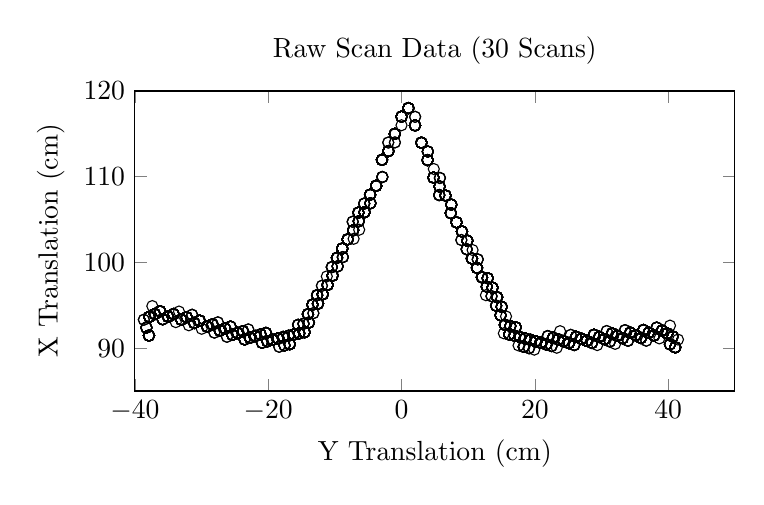
\begin{tikzpicture}

\begin{axis}[%
width=3.0in,
height=1.5in,
scale only axis,
xmin=-40,
xmax=50,
xlabel={Y Translation (cm)},
ymin=85,
ymax=120,
ylabel={X Translation (cm)},
title={Raw Scan Data (30 Scans)}
]
\addplot [
color=black,
only marks,
mark=o,
mark options={solid},
forget plot
]
table[row sep=crcr]{
41.05463 90.08617\\
41.05463 90.08617\\
41.05463 90.08617\\
41.46932 90.99613\\
41.05463 90.08617\\
41.05463 90.08617\\
41.05463 90.08617\\
41.05463 90.08617\\
41.05463 90.08617\\
41.05463 90.08617\\
41.05463 90.08617\\
41.05463 90.08617\\
41.05463 90.08617\\
41.05463 90.08617\\
41.05463 90.08617\\
41.05463 90.08617\\
41.05463 90.08617\\
41.05463 90.08617\\
41.05463 90.08617\\
41.05463 90.08617\\
41.05463 90.08617\\
41.05463 90.08617\\
41.05463 90.08617\\
41.05463 90.08617\\
41.05463 90.08617\\
41.05463 90.08617\\
41.05463 90.08617\\
41.05463 90.08617\\
41.05463 90.08617\\
41.05463 90.08617\\
};
\addplot [
color=black,
only marks,
mark=o,
mark options={solid},
forget plot
]
table[row sep=crcr]{
40.67366 91.35455\\
40.67366 91.35455\\
40.67366 91.35455\\
40.67366 91.35455\\
40.67366 91.35455\\
40.67366 91.35455\\
40.67366 91.35455\\
40.67366 91.35455\\
40.67366 91.35455\\
40.67366 91.35455\\
40.67366 91.35455\\
40.26693 90.441\\
40.26693 90.441\\
40.67366 91.35455\\
40.26693 90.441\\
40.67366 91.35455\\
40.26693 90.441\\
40.26693 90.441\\
40.67366 91.35455\\
40.67366 91.35455\\
40.26693 90.441\\
40.67366 91.35455\\
40.67366 91.35455\\
40.67366 91.35455\\
40.26693 90.441\\
40.67366 91.35455\\
40.26693 90.441\\
40.67366 91.35455\\
40.67366 91.35455\\
40.26693 90.441\\
};
\addplot [
color=black,
only marks,
mark=o,
mark options={solid},
forget plot
]
table[row sep=crcr]{
39.87491 91.70601\\
39.87491 91.70601\\
39.87491 91.70601\\
39.87491 91.70601\\
39.87491 91.70601\\
39.87491 91.70601\\
39.87491 91.70601\\
39.87491 91.70601\\
40.27366 92.62307\\
39.87491 91.70601\\
39.87491 91.70601\\
39.87491 91.70601\\
39.87491 91.70601\\
39.87491 91.70601\\
39.87491 91.70601\\
39.87491 91.70601\\
39.87491 91.70601\\
39.87491 91.70601\\
39.87491 91.70601\\
39.87491 91.70601\\
39.87491 91.70601\\
39.87491 91.70601\\
39.87491 91.70601\\
39.87491 91.70601\\
39.87491 91.70601\\
39.87491 91.70601\\
39.87491 91.70601\\
39.87491 91.70601\\
39.87491 91.70601\\
39.87491 91.70601\\
};
\addplot [
color=black,
only marks,
mark=o,
mark options={solid},
forget plot
]
table[row sep=crcr]{
39.07311 92.05049\\
39.07311 92.05049\\
39.07311 92.05049\\
39.07311 92.05049\\
39.07311 92.05049\\
39.07311 92.05049\\
39.07311 92.05049\\
39.07311 92.05049\\
39.07311 92.05049\\
39.07311 92.05049\\
39.07311 92.05049\\
39.07311 92.05049\\
39.07311 92.05049\\
39.07311 92.05049\\
39.07311 92.05049\\
39.07311 92.05049\\
39.07311 92.05049\\
39.07311 92.05049\\
39.07311 92.05049\\
39.07311 92.05049\\
39.07311 92.05049\\
39.07311 92.05049\\
39.07311 92.05049\\
38.68238 91.12998\\
39.07311 92.05049\\
39.07311 92.05049\\
39.07311 92.05049\\
39.07311 92.05049\\
39.07311 92.05049\\
39.07311 92.05049\\
};
\addplot [
color=black,
only marks,
mark=o,
mark options={solid},
forget plot
]
table[row sep=crcr]{
37.88566 91.46407\\
38.26834 92.38795\\
37.88566 91.46407\\
38.26834 92.38795\\
37.88566 91.46407\\
37.88566 91.46407\\
37.88566 91.46407\\
37.88566 91.46407\\
38.26834 92.38795\\
38.26834 92.38795\\
37.88566 91.46407\\
37.88566 91.46407\\
37.88566 91.46407\\
37.88566 91.46407\\
37.88566 91.46407\\
37.88566 91.46407\\
37.88566 91.46407\\
38.26834 92.38795\\
38.26834 92.38795\\
37.88566 91.46407\\
37.88566 91.46407\\
37.88566 91.46407\\
37.88566 91.46407\\
37.88566 91.46407\\
37.88566 91.46407\\
37.88566 91.46407\\
37.88566 91.46407\\
37.88566 91.46407\\
37.88566 91.46407\\
37.88566 91.46407\\
};
\addplot [
color=black,
only marks,
mark=o,
mark options={solid},
forget plot
]
table[row sep=crcr]{
37.08605 91.7912\\
37.08605 91.7912\\
37.08605 91.7912\\
37.08605 91.7912\\
37.08605 91.7912\\
37.08605 91.7912\\
37.08605 91.7912\\
37.08605 91.7912\\
37.08605 91.7912\\
37.08605 91.7912\\
37.08605 91.7912\\
37.08605 91.7912\\
36.71145 90.86402\\
37.08605 91.7912\\
37.08605 91.7912\\
37.08605 91.7912\\
37.08605 91.7912\\
37.08605 91.7912\\
37.08605 91.7912\\
37.08605 91.7912\\
37.08605 91.7912\\
37.08605 91.7912\\
37.08605 91.7912\\
37.08605 91.7912\\
37.08605 91.7912\\
37.08605 91.7912\\
37.08605 91.7912\\
37.08605 91.7912\\
36.71145 90.86402\\
37.08605 91.7912\\
};
\addplot [
color=black,
only marks,
mark=o,
mark options={solid},
forget plot
]
table[row sep=crcr]{
35.91712 91.18092\\
36.28362 92.11134\\
36.28362 92.11134\\
36.28362 92.11134\\
35.91712 91.18092\\
35.91712 91.18092\\
36.28362 92.11134\\
35.91712 91.18092\\
36.28362 92.11134\\
35.91712 91.18092\\
35.91712 91.18092\\
36.28362 92.11134\\
35.91712 91.18092\\
35.91712 91.18092\\
36.28362 92.11134\\
35.91712 91.18092\\
36.28362 92.11134\\
36.28362 92.11134\\
36.28362 92.11134\\
35.91712 91.18092\\
35.91712 91.18092\\
36.28362 92.11134\\
36.28362 92.11134\\
36.28362 92.11134\\
36.28362 92.11134\\
35.91712 91.18092\\
36.28362 92.11134\\
35.91712 91.18092\\
35.91712 91.18092\\
35.91712 91.18092\\
};
\addplot [
color=black,
only marks,
mark=o,
mark options={solid},
forget plot
]
table[row sep=crcr]{
35.12006 91.49088\\
35.12006 91.49088\\
35.12006 91.49088\\
35.12006 91.49088\\
35.12006 91.49088\\
35.12006 91.49088\\
35.12006 91.49088\\
35.12006 91.49088\\
35.12006 91.49088\\
35.12006 91.49088\\
35.12006 91.49088\\
35.12006 91.49088\\
35.12006 91.49088\\
35.12006 91.49088\\
35.12006 91.49088\\
35.12006 91.49088\\
35.12006 91.49088\\
35.12006 91.49088\\
35.12006 91.49088\\
35.12006 91.49088\\
35.12006 91.49088\\
35.12006 91.49088\\
35.12006 91.49088\\
35.12006 91.49088\\
35.12006 91.49088\\
35.12006 91.49088\\
35.12006 91.49088\\
35.12006 91.49088\\
35.12006 91.49088\\
35.12006 91.49088\\
};
\addplot [
color=black,
only marks,
mark=o,
mark options={solid},
forget plot
]
table[row sep=crcr]{
34.32032 91.79387\\
34.32032 91.79387\\
34.32032 91.79387\\
34.32032 91.79387\\
34.32032 91.79387\\
34.32032 91.79387\\
34.32032 91.79387\\
34.32032 91.79387\\
34.32032 91.79387\\
34.32032 91.79387\\
34.32032 91.79387\\
33.97012 90.8572\\
34.32032 91.79387\\
34.32032 91.79387\\
34.32032 91.79387\\
33.97012 90.8572\\
34.32032 91.79387\\
34.32032 91.79387\\
34.32032 91.79387\\
34.32032 91.79387\\
34.32032 91.79387\\
34.32032 91.79387\\
34.32032 91.79387\\
34.32032 91.79387\\
34.32032 91.79387\\
34.32032 91.79387\\
34.32032 91.79387\\
33.97012 90.8572\\
34.32032 91.79387\\
33.97012 90.8572\\
};
\addplot [
color=black,
only marks,
mark=o,
mark options={solid},
forget plot
]
table[row sep=crcr]{
33.51797 92.08988\\
33.17595 91.15018\\
33.17595 91.15018\\
33.17595 91.15018\\
33.17595 91.15018\\
33.17595 91.15018\\
33.17595 91.15018\\
33.17595 91.15018\\
33.17595 91.15018\\
33.17595 91.15018\\
33.17595 91.15018\\
33.17595 91.15018\\
33.17595 91.15018\\
33.17595 91.15018\\
33.17595 91.15018\\
33.17595 91.15018\\
33.51797 92.08988\\
33.17595 91.15018\\
33.17595 91.15018\\
33.17595 91.15018\\
33.17595 91.15018\\
33.17595 91.15018\\
33.17595 91.15018\\
33.17595 91.15018\\
33.17595 91.15018\\
33.17595 91.15018\\
33.17595 91.15018\\
33.17595 91.15018\\
33.17595 91.15018\\
33.51797 92.08988\\
};
\addplot [
color=black,
only marks,
mark=o,
mark options={solid},
forget plot
]
table[row sep=crcr]{
32.37927 91.43622\\
32.37927 91.43622\\
32.37927 91.43622\\
32.37927 91.43622\\
32.37927 91.43622\\
32.37927 91.43622\\
32.37927 91.43622\\
32.04546 90.49358\\
32.37927 91.43622\\
32.37927 91.43622\\
32.37927 91.43622\\
32.37927 91.43622\\
32.37927 91.43622\\
32.37927 91.43622\\
32.37927 91.43622\\
32.37927 91.43622\\
32.37927 91.43622\\
32.37927 91.43622\\
32.37927 91.43622\\
32.37927 91.43622\\
32.37927 91.43622\\
32.37927 91.43622\\
32.37927 91.43622\\
32.37927 91.43622\\
32.37927 91.43622\\
32.37927 91.43622\\
32.37927 91.43622\\
32.37927 91.43622\\
32.37927 91.43622\\
32.37927 91.43622\\
};
\addplot [
color=black,
only marks,
mark=o,
mark options={solid},
forget plot
]
table[row sep=crcr]{
31.58011 91.7153\\
31.58011 91.7153\\
31.58011 91.7153\\
31.58011 91.7153\\
31.58011 91.7153\\
31.58011 91.7153\\
31.25454 90.76978\\
31.58011 91.7153\\
31.58011 91.7153\\
31.25454 90.76978\\
31.58011 91.7153\\
31.58011 91.7153\\
31.25454 90.76978\\
31.58011 91.7153\\
31.58011 91.7153\\
31.58011 91.7153\\
31.58011 91.7153\\
31.58011 91.7153\\
31.58011 91.7153\\
31.58011 91.7153\\
31.58011 91.7153\\
31.58011 91.7153\\
31.58011 91.7153\\
31.58011 91.7153\\
31.25454 90.76978\\
31.58011 91.7153\\
31.58011 91.7153\\
31.58011 91.7153\\
31.58011 91.7153\\
31.58011 91.7153\\
};
\addplot [
color=black,
only marks,
mark=o,
mark options={solid},
forget plot
]
table[row sep=crcr]{
30.46125 91.03907\\
30.46125 91.03907\\
30.46125 91.03907\\
30.77855 91.98739\\
30.46125 91.03907\\
30.46125 91.03907\\
30.46125 91.03907\\
30.46125 91.03907\\
30.46125 91.03907\\
30.46125 91.03907\\
30.46125 91.03907\\
30.46125 91.03907\\
30.46125 91.03907\\
30.46125 91.03907\\
30.46125 91.03907\\
30.46125 91.03907\\
30.46125 91.03907\\
30.46125 91.03907\\
30.46125 91.03907\\
30.46125 91.03907\\
30.46125 91.03907\\
30.77855 91.98739\\
30.46125 91.03907\\
30.46125 91.03907\\
30.46125 91.03907\\
30.46125 91.03907\\
30.46125 91.03907\\
30.46125 91.03907\\
30.46125 91.03907\\
30.46125 91.03907\\
};
\addplot [
color=black,
only marks,
mark=o,
mark options={solid},
forget plot
]
table[row sep=crcr]{
29.66563 91.30143\\
29.66563 91.30143\\
29.66563 91.30143\\
29.66563 91.30143\\
29.66563 91.30143\\
29.66563 91.30143\\
29.66563 91.30143\\
29.35661 90.35037\\
29.66563 91.30143\\
29.66563 91.30143\\
29.66563 91.30143\\
29.66563 91.30143\\
29.66563 91.30143\\
29.66563 91.30143\\
29.66563 91.30143\\
29.66563 91.30143\\
29.66563 91.30143\\
29.66563 91.30143\\
29.66563 91.30143\\
29.66563 91.30143\\
29.66563 91.30143\\
29.66563 91.30143\\
29.66563 91.30143\\
29.66563 91.30143\\
29.66563 91.30143\\
29.66563 91.30143\\
29.66563 91.30143\\
29.66563 91.30143\\
29.66563 91.30143\\
29.66563 91.30143\\
};
\addplot [
color=black,
only marks,
mark=o,
mark options={solid},
forget plot
]
table[row sep=crcr]{
28.86776 91.55683\\
28.86776 91.55683\\
28.56705 90.60311\\
28.86776 91.55683\\
28.56705 90.60311\\
28.86776 91.55683\\
28.56705 90.60311\\
28.56705 90.60311\\
28.86776 91.55683\\
28.86776 91.55683\\
28.86776 91.55683\\
28.86776 91.55683\\
28.86776 91.55683\\
28.86776 91.55683\\
28.56705 90.60311\\
28.56705 90.60311\\
28.86776 91.55683\\
28.56705 90.60311\\
28.56705 90.60311\\
28.86776 91.55683\\
28.86776 91.55683\\
28.86776 91.55683\\
28.86776 91.55683\\
28.86776 91.55683\\
28.56705 90.60311\\
28.86776 91.55683\\
28.86776 91.55683\\
28.56705 90.60311\\
28.86776 91.55683\\
28.56705 90.60311\\
};
\addplot [
color=black,
only marks,
mark=o,
mark options={solid},
forget plot
]
table[row sep=crcr]{
27.77531 90.84895\\
27.77531 90.84895\\
27.77531 90.84895\\
27.77531 90.84895\\
27.77531 90.84895\\
27.77531 90.84895\\
27.77531 90.84895\\
27.77531 90.84895\\
27.77531 90.84895\\
27.77531 90.84895\\
27.77531 90.84895\\
27.77531 90.84895\\
27.77531 90.84895\\
27.77531 90.84895\\
27.77531 90.84895\\
27.77531 90.84895\\
27.77531 90.84895\\
27.77531 90.84895\\
27.77531 90.84895\\
27.77531 90.84895\\
27.77531 90.84895\\
27.77531 90.84895\\
27.77531 90.84895\\
27.77531 90.84895\\
27.77531 90.84895\\
27.77531 90.84895\\
27.77531 90.84895\\
27.77531 90.84895\\
27.77531 90.84895\\
27.77531 90.84895\\
};
\addplot [
color=black,
only marks,
mark=o,
mark options={solid},
forget plot
]
table[row sep=crcr]{
26.98146 91.08787\\
26.98146 91.08787\\
26.98146 91.08787\\
26.98146 91.08787\\
26.98146 91.08787\\
26.98146 91.08787\\
26.98146 91.08787\\
26.98146 91.08787\\
26.98146 91.08787\\
26.98146 91.08787\\
26.98146 91.08787\\
26.98146 91.08787\\
26.98146 91.08787\\
26.98146 91.08787\\
26.98146 91.08787\\
26.98146 91.08787\\
26.98146 91.08787\\
26.98146 91.08787\\
26.98146 91.08787\\
26.98146 91.08787\\
26.98146 91.08787\\
26.98146 91.08787\\
26.98146 91.08787\\
26.98146 91.08787\\
26.98146 91.08787\\
26.98146 91.08787\\
26.98146 91.08787\\
26.98146 91.08787\\
26.98146 91.08787\\
26.98146 91.08787\\
};
\addplot [
color=black,
only marks,
mark=o,
mark options={solid},
forget plot
]
table[row sep=crcr]{
25.90991 90.3586\\
26.18555 91.31986\\
25.90991 90.3586\\
26.18555 91.31986\\
26.18555 91.31986\\
26.18555 91.31986\\
26.18555 91.31986\\
26.18555 91.31986\\
25.90991 90.3586\\
25.90991 90.3586\\
26.18555 91.31986\\
26.18555 91.31986\\
26.18555 91.31986\\
25.90991 90.3586\\
25.90991 90.3586\\
26.18555 91.31986\\
26.18555 91.31986\\
26.18555 91.31986\\
26.18555 91.31986\\
26.18555 91.31986\\
26.18555 91.31986\\
26.18555 91.31986\\
25.90991 90.3586\\
26.18555 91.31986\\
26.18555 91.31986\\
26.18555 91.31986\\
26.18555 91.31986\\
26.18555 91.31986\\
26.18555 91.31986\\
26.18555 91.31986\\
};
\addplot [
color=black,
only marks,
mark=o,
mark options={solid},
forget plot
]
table[row sep=crcr]{
25.12041 90.58126\\
25.38765 91.54489\\
25.38765 91.54489\\
25.12041 90.58126\\
25.12041 90.58126\\
25.12041 90.58126\\
25.12041 90.58126\\
25.12041 90.58126\\
25.12041 90.58126\\
25.12041 90.58126\\
25.12041 90.58126\\
25.12041 90.58126\\
25.12041 90.58126\\
25.12041 90.58126\\
25.12041 90.58126\\
25.12041 90.58126\\
25.12041 90.58126\\
25.12041 90.58126\\
25.12041 90.58126\\
25.12041 90.58126\\
25.12041 90.58126\\
25.12041 90.58126\\
25.12041 90.58126\\
25.12041 90.58126\\
25.12041 90.58126\\
25.12041 90.58126\\
25.12041 90.58126\\
25.12041 90.58126\\
25.12041 90.58126\\
25.12041 90.58126\\
};
\addplot [
color=black,
only marks,
mark=o,
mark options={solid},
forget plot
]
table[row sep=crcr]{
24.32899 90.79703\\
24.32899 90.79703\\
24.32899 90.79703\\
24.32899 90.79703\\
24.32899 90.79703\\
24.32899 90.79703\\
24.32899 90.79703\\
24.32899 90.79703\\
24.32899 90.79703\\
24.32899 90.79703\\
24.32899 90.79703\\
24.32899 90.79703\\
24.32899 90.79703\\
24.32899 90.79703\\
24.32899 90.79703\\
24.32899 90.79703\\
24.32899 90.79703\\
24.32899 90.79703\\
24.32899 90.79703\\
24.32899 90.79703\\
24.32899 90.79703\\
24.32899 90.79703\\
24.32899 90.79703\\
24.32899 90.79703\\
24.32899 90.79703\\
24.32899 90.79703\\
24.32899 90.79703\\
24.32899 90.79703\\
24.32899 90.79703\\
24.32899 90.79703\\
};
\addplot [
color=black,
only marks,
mark=o,
mark options={solid},
forget plot
]
table[row sep=crcr]{
23.7861 91.97403\\
23.53572 91.00588\\
23.53572 91.00588\\
23.53572 91.00588\\
23.53572 91.00588\\
23.53572 91.00588\\
23.53572 91.00588\\
23.53572 91.00588\\
23.53572 91.00588\\
23.53572 91.00588\\
23.53572 91.00588\\
23.53572 91.00588\\
23.53572 91.00588\\
23.53572 91.00588\\
23.53572 91.00588\\
23.53572 91.00588\\
23.53572 91.00588\\
23.53572 91.00588\\
23.28534 90.03773\\
23.53572 91.00588\\
23.53572 91.00588\\
23.53572 91.00588\\
23.53572 91.00588\\
23.53572 91.00588\\
23.53572 91.00588\\
23.53572 91.00588\\
23.53572 91.00588\\
23.53572 91.00588\\
23.53572 91.00588\\
23.53572 91.00588\\
};
\addplot [
color=black,
only marks,
mark=o,
mark options={solid},
forget plot
]
table[row sep=crcr]{
22.74066 91.2078\\
22.74066 91.2078\\
22.74066 91.2078\\
22.49874 90.2375\\
22.74066 91.2078\\
22.74066 91.2078\\
22.74066 91.2078\\
22.74066 91.2078\\
22.49874 90.2375\\
22.74066 91.2078\\
22.74066 91.2078\\
22.74066 91.2078\\
22.74066 91.2078\\
22.74066 91.2078\\
22.74066 91.2078\\
22.49874 90.2375\\
22.74066 91.2078\\
22.74066 91.2078\\
22.74066 91.2078\\
22.74066 91.2078\\
22.49874 90.2375\\
22.49874 90.2375\\
22.74066 91.2078\\
22.74066 91.2078\\
22.74066 91.2078\\
22.74066 91.2078\\
22.74066 91.2078\\
22.74066 91.2078\\
22.74066 91.2078\\
22.74066 91.2078\\
};
\addplot [
color=black,
only marks,
mark=o,
mark options={solid},
forget plot
]
table[row sep=crcr]{
21.71042 90.4304\\
21.71042 90.4304\\
21.71042 90.4304\\
21.71042 90.4304\\
21.94386 91.40277\\
21.71042 90.4304\\
21.71042 90.4304\\
21.94386 91.40277\\
21.71042 90.4304\\
21.71042 90.4304\\
21.71042 90.4304\\
21.71042 90.4304\\
21.71042 90.4304\\
21.71042 90.4304\\
21.71042 90.4304\\
21.71042 90.4304\\
21.71042 90.4304\\
21.71042 90.4304\\
21.71042 90.4304\\
21.71042 90.4304\\
21.71042 90.4304\\
21.71042 90.4304\\
21.71042 90.4304\\
21.94386 91.40277\\
21.71042 90.4304\\
21.71042 90.4304\\
21.94386 91.40277\\
21.71042 90.4304\\
21.71042 90.4304\\
21.71042 90.4304\\
};
\addplot [
color=black,
only marks,
mark=o,
mark options={solid},
forget plot
]
table[row sep=crcr]{
20.92045 90.61642\\
20.92045 90.61642\\
20.92045 90.61642\\
20.92045 90.61642\\
20.92045 90.61642\\
20.92045 90.61642\\
20.92045 90.61642\\
20.92045 90.61642\\
20.92045 90.61642\\
20.92045 90.61642\\
20.92045 90.61642\\
20.92045 90.61642\\
20.92045 90.61642\\
20.92045 90.61642\\
20.92045 90.61642\\
20.92045 90.61642\\
20.92045 90.61642\\
20.92045 90.61642\\
20.92045 90.61642\\
20.92045 90.61642\\
20.92045 90.61642\\
20.92045 90.61642\\
20.92045 90.61642\\
20.92045 90.61642\\
20.92045 90.61642\\
20.92045 90.61642\\
20.92045 90.61642\\
20.92045 90.61642\\
20.92045 90.61642\\
20.92045 90.61642\\
};
\addplot [
color=black,
only marks,
mark=o,
mark options={solid},
forget plot
]
table[row sep=crcr]{
20.12888 90.79553\\
20.12888 90.79553\\
20.12888 90.79553\\
20.12888 90.79553\\
20.12888 90.79553\\
20.12888 90.79553\\
20.12888 90.79553\\
19.91244 89.81923\\
20.12888 90.79553\\
20.12888 90.79553\\
20.12888 90.79553\\
20.12888 90.79553\\
20.12888 90.79553\\
20.12888 90.79553\\
20.12888 90.79553\\
20.12888 90.79553\\
20.12888 90.79553\\
20.12888 90.79553\\
20.12888 90.79553\\
20.12888 90.79553\\
20.12888 90.79553\\
20.12888 90.79553\\
20.12888 90.79553\\
20.12888 90.79553\\
20.12888 90.79553\\
20.12888 90.79553\\
20.12888 90.79553\\
20.12888 90.79553\\
20.12888 90.79553\\
20.12888 90.79553\\
};
\addplot [
color=black,
only marks,
mark=o,
mark options={solid},
forget plot
]
table[row sep=crcr]{
19.33579 90.96773\\
19.33579 90.96773\\
19.33579 90.96773\\
19.33579 90.96773\\
19.33579 90.96773\\
19.33579 90.96773\\
19.33579 90.96773\\
19.12788 89.98958\\
19.33579 90.96773\\
19.33579 90.96773\\
19.12788 89.98958\\
19.33579 90.96773\\
19.33579 90.96773\\
19.33579 90.96773\\
19.33579 90.96773\\
19.12788 89.98958\\
19.33579 90.96773\\
19.33579 90.96773\\
19.33579 90.96773\\
19.33579 90.96773\\
19.33579 90.96773\\
19.33579 90.96773\\
19.33579 90.96773\\
19.33579 90.96773\\
19.33579 90.96773\\
19.33579 90.96773\\
19.12788 89.98958\\
19.33579 90.96773\\
19.33579 90.96773\\
19.33579 90.96773\\
};
\addplot [
color=black,
only marks,
mark=o,
mark options={solid},
forget plot
]
table[row sep=crcr]{
18.34185 90.15307\\
18.34185 90.15307\\
18.34185 90.15307\\
18.54122 91.133\\
18.34185 90.15307\\
18.54122 91.133\\
18.34185 90.15307\\
18.54122 91.133\\
18.54122 91.133\\
18.54122 91.133\\
18.34185 90.15307\\
18.34185 90.15307\\
18.54122 91.133\\
18.34185 90.15307\\
18.34185 90.15307\\
18.54122 91.133\\
18.34185 90.15307\\
18.54122 91.133\\
18.34185 90.15307\\
18.34185 90.15307\\
18.34185 90.15307\\
18.34185 90.15307\\
18.34185 90.15307\\
18.54122 91.133\\
18.34185 90.15307\\
18.34185 90.15307\\
18.54122 91.133\\
18.54122 91.133\\
18.34185 90.15307\\
18.54122 91.133\\
};
\addplot [
color=black,
only marks,
mark=o,
mark options={solid},
forget plot
]
table[row sep=crcr]{
17.74524 91.29133\\
17.74524 91.29133\\
17.74524 91.29133\\
17.74524 91.29133\\
17.74524 91.29133\\
17.74524 91.29133\\
17.74524 91.29133\\
17.74524 91.29133\\
17.74524 91.29133\\
17.74524 91.29133\\
17.74524 91.29133\\
17.74524 91.29133\\
17.74524 91.29133\\
17.74524 91.29133\\
17.74524 91.29133\\
17.74524 91.29133\\
17.74524 91.29133\\
17.74524 91.29133\\
17.74524 91.29133\\
17.74524 91.29133\\
17.74524 91.29133\\
17.74524 91.29133\\
17.74524 91.29133\\
17.74524 91.29133\\
17.74524 91.29133\\
17.74524 91.29133\\
17.55443 90.3097\\
17.74524 91.29133\\
17.74524 91.29133\\
17.74524 91.29133\\
};
\addplot [
color=black,
only marks,
mark=o,
mark options={solid},
forget plot
]
table[row sep=crcr]{
17.13014 92.42596\\
16.9479 91.44271\\
16.9479 91.44271\\
16.9479 91.44271\\
16.9479 91.44271\\
16.9479 91.44271\\
17.13014 92.42596\\
17.13014 92.42596\\
17.13014 92.42596\\
16.9479 91.44271\\
17.13014 92.42596\\
17.13014 92.42596\\
16.9479 91.44271\\
16.9479 91.44271\\
17.13014 92.42596\\
16.9479 91.44271\\
17.13014 92.42596\\
17.13014 92.42596\\
17.13014 92.42596\\
16.9479 91.44271\\
16.9479 91.44271\\
17.13014 92.42596\\
16.9479 91.44271\\
17.13014 92.42596\\
16.9479 91.44271\\
16.9479 91.44271\\
17.13014 92.42596\\
17.13014 92.42596\\
16.9479 91.44271\\
16.9479 91.44271\\
};
\addplot [
color=black,
only marks,
mark=o,
mark options={solid},
forget plot
]
table[row sep=crcr]{
16.32293 92.57193\\
16.32293 92.57193\\
16.14928 91.58712\\
16.32293 92.57193\\
16.14928 91.58712\\
16.32293 92.57193\\
16.14928 91.58712\\
16.14928 91.58712\\
16.14928 91.58712\\
16.14928 91.58712\\
16.32293 92.57193\\
16.14928 91.58712\\
16.14928 91.58712\\
16.14928 91.58712\\
16.14928 91.58712\\
16.14928 91.58712\\
16.14928 91.58712\\
16.14928 91.58712\\
16.32293 92.57193\\
16.14928 91.58712\\
16.32293 92.57193\\
16.14928 91.58712\\
16.32293 92.57193\\
16.32293 92.57193\\
16.14928 91.58712\\
16.14928 91.58712\\
16.14928 91.58712\\
16.14928 91.58712\\
16.32293 92.57193\\
16.14928 91.58712\\
};
\addplot [
color=black,
only marks,
mark=o,
mark options={solid},
forget plot
]
table[row sep=crcr]{
15.51447 92.71085\\
15.51447 92.71085\\
15.51447 92.71085\\
15.51447 92.71085\\
15.51447 92.71085\\
15.51447 92.71085\\
15.51447 92.71085\\
15.51447 92.71085\\
15.51447 92.71085\\
15.51447 92.71085\\
15.51447 92.71085\\
15.51447 92.71085\\
15.51447 92.71085\\
15.51447 92.71085\\
15.51447 92.71085\\
15.51447 92.71085\\
15.51447 92.71085\\
15.51447 92.71085\\
15.67952 93.69713\\
15.51447 92.71085\\
15.51447 92.71085\\
15.34943 91.72456\\
15.51447 92.71085\\
15.51447 92.71085\\
15.51447 92.71085\\
15.51447 92.71085\\
15.51447 92.71085\\
15.51447 92.71085\\
15.51447 92.71085\\
15.51447 92.71085\\
};
\addplot [
color=black,
only marks,
mark=o,
mark options={solid},
forget plot
]
table[row sep=crcr]{
15.01771 94.81808\\
15.01771 94.81808\\
15.01771 94.81808\\
15.01771 94.81808\\
14.86127 93.83039\\
15.01771 94.81808\\
14.86127 93.83039\\
15.01771 94.81808\\
14.86127 93.83039\\
15.01771 94.81808\\
14.86127 93.83039\\
14.86127 93.83039\\
14.86127 93.83039\\
14.86127 93.83039\\
14.86127 93.83039\\
14.86127 93.83039\\
15.01771 94.81808\\
15.01771 94.81808\\
14.86127 93.83039\\
15.01771 94.81808\\
14.86127 93.83039\\
14.86127 93.83039\\
15.01771 94.81808\\
15.01771 94.81808\\
14.86127 93.83039\\
14.86127 93.83039\\
14.86127 93.83039\\
15.01771 94.81808\\
15.01771 94.81808\\
14.86127 93.83039\\
};
\addplot [
color=black,
only marks,
mark=o,
mark options={solid},
forget plot
]
table[row sep=crcr]{
14.33751 95.93454\\
14.1897 94.94552\\
14.33751 95.93454\\
14.1897 94.94552\\
14.1897 94.94552\\
14.33751 95.93454\\
14.33751 95.93454\\
14.33751 95.93454\\
14.1897 94.94552\\
14.33751 95.93454\\
14.33751 95.93454\\
14.33751 95.93454\\
14.33751 95.93454\\
14.1897 94.94552\\
14.1897 94.94552\\
14.1897 94.94552\\
14.33751 95.93454\\
14.33751 95.93454\\
14.33751 95.93454\\
14.33751 95.93454\\
14.1897 94.94552\\
14.33751 95.93454\\
14.33751 95.93454\\
14.33751 95.93454\\
14.33751 95.93454\\
14.33751 95.93454\\
14.33751 95.93454\\
14.1897 94.94552\\
14.33751 95.93454\\
14.33751 95.93454\\
};
\addplot [
color=black,
only marks,
mark=o,
mark options={solid},
forget plot
]
table[row sep=crcr]{
13.63896 97.04627\\
13.63896 97.04627\\
13.63896 97.04627\\
13.63896 97.04627\\
13.63896 97.04627\\
13.63896 97.04627\\
13.63896 97.04627\\
13.49979 96.056\\
13.63896 97.04627\\
13.63896 97.04627\\
13.63896 97.04627\\
13.63896 97.04627\\
13.63896 97.04627\\
13.63896 97.04627\\
13.63896 97.04627\\
13.63896 97.04627\\
13.63896 97.04627\\
13.63896 97.04627\\
13.63896 97.04627\\
13.63896 97.04627\\
13.63896 97.04627\\
13.63896 97.04627\\
13.63896 97.04627\\
13.63896 97.04627\\
13.63896 97.04627\\
13.49979 96.056\\
13.63896 97.04627\\
13.63896 97.04627\\
13.63896 97.04627\\
13.49979 96.056\\
};
\addplot [
color=black,
only marks,
mark=o,
mark options={solid},
forget plot
]
table[row sep=crcr]{
12.92209 98.15304\\
12.92209 98.15304\\
12.92209 98.15304\\
12.92209 98.15304\\
12.66104 96.17015\\
12.79157 97.1616\\
12.92209 98.15304\\
12.92209 98.15304\\
12.79157 97.1616\\
12.92209 98.15304\\
12.79157 97.1616\\
12.79157 97.1616\\
12.79157 97.1616\\
12.79157 97.1616\\
12.79157 97.1616\\
12.92209 98.15304\\
12.92209 98.15304\\
12.92209 98.15304\\
12.92209 98.15304\\
12.79157 97.1616\\
12.79157 97.1616\\
12.92209 98.15304\\
12.79157 97.1616\\
12.79157 97.1616\\
12.92209 98.15304\\
12.79157 97.1616\\
12.92209 98.15304\\
12.79157 97.1616\\
12.79157 97.1616\\
12.92209 98.15304\\
};
\addplot [
color=black,
only marks,
mark=o,
mark options={solid},
forget plot
]
table[row sep=crcr]{
12.06506 98.26207\\
12.06506 98.26207\\
12.06506 98.26207\\
12.06506 98.26207\\
12.06506 98.26207\\
12.06506 98.26207\\
12.06506 98.26207\\
12.06506 98.26207\\
12.06506 98.26207\\
12.06506 98.26207\\
12.06506 98.26207\\
12.06506 98.26207\\
12.06506 98.26207\\
12.06506 98.26207\\
12.06506 98.26207\\
12.06506 98.26207\\
12.06506 98.26207\\
12.06506 98.26207\\
12.06506 98.26207\\
12.06506 98.26207\\
12.06506 98.26207\\
12.06506 98.26207\\
12.06506 98.26207\\
12.06506 98.26207\\
12.06506 98.26207\\
12.06506 98.26207\\
12.06506 98.26207\\
12.06506 98.26207\\
12.06506 98.26207\\
12.06506 98.26207\\
};
\addplot [
color=black,
only marks,
mark=o,
mark options={solid},
forget plot
]
table[row sep=crcr]{
11.32032 99.35719\\
11.32032 99.35719\\
11.32032 99.35719\\
11.43352 100.3508\\
11.32032 99.35719\\
11.32032 99.35719\\
11.32032 99.35719\\
11.43352 100.3508\\
11.32032 99.35719\\
11.32032 99.35719\\
11.32032 99.35719\\
11.32032 99.35719\\
11.32032 99.35719\\
11.32032 99.35719\\
11.32032 99.35719\\
11.32032 99.35719\\
11.32032 99.35719\\
11.32032 99.35719\\
11.43352 100.3508\\
11.32032 99.35719\\
11.32032 99.35719\\
11.32032 99.35719\\
11.32032 99.35719\\
11.32032 99.35719\\
11.32032 99.35719\\
11.32032 99.35719\\
11.32032 99.35719\\
11.32032 99.35719\\
11.32032 99.35719\\
11.32032 99.35719\\
};
\addplot [
color=black,
only marks,
mark=o,
mark options={solid},
forget plot
]
table[row sep=crcr]{
10.55737 100.4467\\
10.55737 100.4467\\
10.6619 101.4412\\
10.55737 100.4467\\
10.55737 100.4467\\
10.55737 100.4467\\
10.55737 100.4467\\
10.55737 100.4467\\
10.55737 100.4467\\
10.55737 100.4467\\
10.55737 100.4467\\
10.55737 100.4467\\
10.55737 100.4467\\
10.55737 100.4467\\
10.55737 100.4467\\
10.55737 100.4467\\
10.55737 100.4467\\
10.55737 100.4467\\
10.55737 100.4467\\
10.55737 100.4467\\
10.55737 100.4467\\
10.55737 100.4467\\
10.55737 100.4467\\
10.55737 100.4467\\
10.55737 100.4467\\
10.55737 100.4467\\
10.55737 100.4467\\
10.55737 100.4467\\
10.55737 100.4467\\
10.55737 100.4467\\
};
\addplot [
color=black,
only marks,
mark=o,
mark options={solid},
forget plot
]
table[row sep=crcr]{
9.872113 102.5258\\
9.872113 102.5258\\
9.872113 102.5258\\
9.872113 102.5258\\
9.872113 102.5258\\
9.872113 102.5258\\
9.872113 102.5258\\
9.872113 102.5258\\
9.872113 102.5258\\
9.872113 102.5258\\
9.776267 101.5304\\
9.872113 102.5258\\
9.872113 102.5258\\
9.872113 102.5258\\
9.872113 102.5258\\
9.776267 101.5304\\
9.776267 101.5304\\
9.776267 101.5304\\
9.872113 102.5258\\
9.872113 102.5258\\
9.872113 102.5258\\
9.872113 102.5258\\
9.872113 102.5258\\
9.776267 101.5304\\
9.872113 102.5258\\
9.872113 102.5258\\
9.872113 102.5258\\
9.872113 102.5258\\
9.872113 102.5258\\
9.776267 101.5304\\
};
\addplot [
color=black,
only marks,
mark=o,
mark options={solid},
forget plot
]
table[row sep=crcr]{
9.064197 103.6042\\
9.064197 103.6042\\
9.064197 103.6042\\
9.064197 103.6042\\
9.064197 103.6042\\
9.064197 103.6042\\
9.064197 103.6042\\
9.064197 103.6042\\
9.064197 103.6042\\
9.064197 103.6042\\
9.064197 103.6042\\
8.977042 102.6081\\
9.064197 103.6042\\
9.064197 103.6042\\
9.064197 103.6042\\
9.064197 103.6042\\
9.064197 103.6042\\
9.064197 103.6042\\
9.064197 103.6042\\
9.064197 103.6042\\
9.064197 103.6042\\
9.064197 103.6042\\
9.064197 103.6042\\
9.064197 103.6042\\
9.064197 103.6042\\
9.064197 103.6042\\
9.064197 103.6042\\
9.064197 103.6042\\
8.977042 102.6081\\
9.064197 103.6042\\
};
\addplot [
color=black,
only marks,
mark=o,
mark options={solid},
forget plot
]
table[row sep=crcr]{
8.238205 104.6763\\
8.238205 104.6763\\
8.238205 104.6763\\
8.238205 104.6763\\
8.238205 104.6763\\
8.238205 104.6763\\
8.238205 104.6763\\
8.238205 104.6763\\
8.238205 104.6763\\
8.238205 104.6763\\
8.238205 104.6763\\
8.238205 104.6763\\
8.238205 104.6763\\
8.238205 104.6763\\
8.238205 104.6763\\
8.238205 104.6763\\
8.238205 104.6763\\
8.238205 104.6763\\
8.238205 104.6763\\
8.238205 104.6763\\
8.238205 104.6763\\
8.238205 104.6763\\
8.238205 104.6763\\
8.238205 104.6763\\
8.238205 104.6763\\
8.238205 104.6763\\
8.238205 104.6763\\
8.238205 104.6763\\
8.238205 104.6763\\
8.238205 104.6763\\
};
\addplot [
color=black,
only marks,
mark=o,
mark options={solid},
forget plot
]
table[row sep=crcr]{
7.463943 106.7394\\
7.394186 105.7418\\
7.463943 106.7394\\
7.394186 105.7418\\
7.394186 105.7418\\
7.394186 105.7418\\
7.394186 105.7418\\
7.394186 105.7418\\
7.394186 105.7418\\
7.394186 105.7418\\
7.463943 106.7394\\
7.394186 105.7418\\
7.394186 105.7418\\
7.463943 106.7394\\
7.394186 105.7418\\
7.394186 105.7418\\
7.463943 106.7394\\
7.394186 105.7418\\
7.463943 106.7394\\
7.463943 106.7394\\
7.463943 106.7394\\
7.463943 106.7394\\
7.394186 105.7418\\
7.394186 105.7418\\
7.463943 106.7394\\
7.394186 105.7418\\
7.463943 106.7394\\
7.463943 106.7394\\
7.463943 106.7394\\
7.394186 105.7418\\
};
\addplot [
color=black,
only marks,
mark=o,
mark options={solid},
forget plot
]
table[row sep=crcr]{
6.593242 107.7986\\
6.593242 107.7986\\
6.593242 107.7986\\
6.593242 107.7986\\
6.593242 107.7986\\
6.593242 107.7986\\
6.593242 107.7986\\
6.593242 107.7986\\
6.593242 107.7986\\
6.593242 107.7986\\
6.593242 107.7986\\
6.593242 107.7986\\
6.593242 107.7986\\
6.593242 107.7986\\
6.593242 107.7986\\
6.593242 107.7986\\
6.593242 107.7986\\
6.593242 107.7986\\
6.593242 107.7986\\
6.593242 107.7986\\
6.593242 107.7986\\
6.593242 107.7986\\
6.593242 107.7986\\
6.593242 107.7986\\
6.593242 107.7986\\
6.593242 107.7986\\
6.593242 107.7986\\
6.593242 107.7986\\
6.593242 107.7986\\
6.593242 107.7986\\
};
\addplot [
color=black,
only marks,
mark=o,
mark options={solid},
forget plot
]
table[row sep=crcr]{
5.704619 108.8506\\
5.704619 108.8506\\
5.704619 108.8506\\
5.704619 108.8506\\
5.704619 108.8506\\
5.704619 108.8506\\
5.704619 108.8506\\
5.704619 108.8506\\
5.652283 107.852\\
5.704619 108.8506\\
5.652283 107.852\\
5.652283 107.852\\
5.704619 108.8506\\
5.756955 109.8492\\
5.704619 108.8506\\
5.704619 108.8506\\
5.704619 108.8506\\
5.756955 109.8492\\
5.704619 108.8506\\
5.704619 108.8506\\
5.704619 108.8506\\
5.652283 107.852\\
5.704619 108.8506\\
5.652283 107.852\\
5.652283 107.852\\
5.704619 108.8506\\
5.704619 108.8506\\
5.704619 108.8506\\
5.756955 109.8492\\
5.652283 107.852\\
};
\addplot [
color=black,
only marks,
mark=o,
mark options={solid},
forget plot
]
table[row sep=crcr]{
4.798133 109.8953\\
4.798133 109.8953\\
4.798133 109.8953\\
4.798133 109.8953\\
4.798133 109.8953\\
4.798133 109.8953\\
4.841752 110.8944\\
4.798133 109.8953\\
4.798133 109.8953\\
4.798133 109.8953\\
4.798133 109.8953\\
4.798133 109.8953\\
4.798133 109.8953\\
4.798133 109.8953\\
4.798133 109.8953\\
4.798133 109.8953\\
4.798133 109.8953\\
4.798133 109.8953\\
4.798133 109.8953\\
4.798133 109.8953\\
4.798133 109.8953\\
4.798133 109.8953\\
4.798133 109.8953\\
4.798133 109.8953\\
4.798133 109.8953\\
4.798133 109.8953\\
4.798133 109.8953\\
4.798133 109.8953\\
4.798133 109.8953\\
4.798133 109.8953\\
};
\addplot [
color=black,
only marks,
mark=o,
mark options={solid},
forget plot
]
table[row sep=crcr]{
3.943643 112.9312\\
3.908744 111.9318\\
3.908744 111.9318\\
3.908744 111.9318\\
3.908744 111.9318\\
3.908744 111.9318\\
3.908744 111.9318\\
3.908744 111.9318\\
3.908744 111.9318\\
3.943643 112.9312\\
3.908744 111.9318\\
3.908744 111.9318\\
3.908744 111.9318\\
3.908744 111.9318\\
3.943643 112.9312\\
3.943643 112.9312\\
3.908744 111.9318\\
3.908744 111.9318\\
3.943643 112.9312\\
3.908744 111.9318\\
3.908744 111.9318\\
3.908744 111.9318\\
3.943643 112.9312\\
3.908744 111.9318\\
3.908744 111.9318\\
3.908744 111.9318\\
3.943643 112.9312\\
3.943643 112.9312\\
3.908744 111.9318\\
3.908744 111.9318\\
};
\addplot [
color=black,
only marks,
mark=o,
mark options={solid},
forget plot
]
table[row sep=crcr]{
2.984172 113.9609\\
2.984172 113.9609\\
2.984172 113.9609\\
2.984172 113.9609\\
2.984172 113.9609\\
2.984172 113.9609\\
2.984172 113.9609\\
2.984172 113.9609\\
2.984172 113.9609\\
2.984172 113.9609\\
2.984172 113.9609\\
2.984172 113.9609\\
2.984172 113.9609\\
2.984172 113.9609\\
2.984172 113.9609\\
2.984172 113.9609\\
2.984172 113.9609\\
2.984172 113.9609\\
2.984172 113.9609\\
2.984172 113.9609\\
2.984172 113.9609\\
2.984172 113.9609\\
2.984172 113.9609\\
2.984172 113.9609\\
2.984172 113.9609\\
2.984172 113.9609\\
2.984172 113.9609\\
2.984172 113.9609\\
2.984172 113.9609\\
2.984172 113.9609\\
};
\addplot [
color=black,
only marks,
mark=o,
mark options={solid},
forget plot
]
table[row sep=crcr]{
2.024479 115.9823\\
2.024479 115.9823\\
2.024479 115.9823\\
2.024479 115.9823\\
2.024479 115.9823\\
2.024479 115.9823\\
2.024479 115.9823\\
2.024479 115.9823\\
2.024479 115.9823\\
2.024479 115.9823\\
2.024479 115.9823\\
2.024479 115.9823\\
2.024479 115.9823\\
2.024479 115.9823\\
2.024479 115.9823\\
2.024479 115.9823\\
2.024479 115.9823\\
2.024479 115.9823\\
2.024479 115.9823\\
2.024479 115.9823\\
2.024479 115.9823\\
2.024479 115.9823\\
2.041932 116.9822\\
2.024479 115.9823\\
2.024479 115.9823\\
2.041932 116.9822\\
2.024479 115.9823\\
2.024479 115.9823\\
2.024479 115.9823\\
2.024479 115.9823\\
};
\addplot [
color=black,
only marks,
mark=o,
mark options={solid},
forget plot
]
table[row sep=crcr]{
1.029731 117.9955\\
1.029731 117.9955\\
1.029731 117.9955\\
1.029731 117.9955\\
1.029731 117.9955\\
1.029731 117.9955\\
1.029731 117.9955\\
1.029731 117.9955\\
1.029731 117.9955\\
1.029731 117.9955\\
1.029731 117.9955\\
1.029731 117.9955\\
1.029731 117.9955\\
1.029731 117.9955\\
1.029731 117.9955\\
1.029731 117.9955\\
1.029731 117.9955\\
1.029731 117.9955\\
1.029731 117.9955\\
1.029731 117.9955\\
1.029731 117.9955\\
1.029731 117.9955\\
1.029731 117.9955\\
1.029731 117.9955\\
1.029731 117.9955\\
1.029731 117.9955\\
1.029731 117.9955\\
1.029731 117.9955\\
1.029731 117.9955\\
1.029731 117.9955\\
};
\addplot [
color=black,
only marks,
mark=o,
mark options={solid},
forget plot
]
table[row sep=crcr]{
0 117\\
0 117\\
0 117\\
0 117\\
0 117\\
0 117\\
0 117\\
0 117\\
0 117\\
0 117\\
0 117\\
0 117\\
0 117\\
0 117\\
0 117\\
0 117\\
0 117\\
0 117\\
0 117\\
0 117\\
0 117\\
0 117\\
0 116\\
0 117\\
0 117\\
0 117\\
0 117\\
0 117\\
0 117\\
0 117\\
};
\addplot [
color=black,
only marks,
mark=o,
mark options={solid},
forget plot
]
table[row sep=crcr]{
-1.003552 114.9956\\
-1.003552 114.9956\\
-1.003552 114.9956\\
-1.003552 114.9956\\
-1.003552 114.9956\\
-1.003552 114.9956\\
-1.003552 114.9956\\
-1.003552 114.9956\\
-1.003552 114.9956\\
-1.003552 114.9956\\
-1.003552 114.9956\\
-1.003552 114.9956\\
-1.003552 114.9956\\
-1.003552 114.9956\\
-1.003552 114.9956\\
-1.003552 114.9956\\
-1.003552 114.9956\\
-1.003552 114.9956\\
-0.994825 113.9957\\
-1.003552 114.9956\\
-1.003552 114.9956\\
-1.003552 114.9956\\
-1.003552 114.9956\\
-0.994825 113.9957\\
-1.003552 114.9956\\
-1.003552 114.9956\\
-1.003552 114.9956\\
-1.003552 114.9956\\
-1.003552 114.9956\\
-1.003552 114.9956\\
};
\addplot [
color=black,
only marks,
mark=o,
mark options={solid},
forget plot
]
table[row sep=crcr]{
-1.972122 112.9828\\
-1.972122 112.9828\\
-1.972122 112.9828\\
-1.972122 112.9828\\
-1.972122 112.9828\\
-1.972122 112.9828\\
-1.972122 112.9828\\
-1.972122 112.9828\\
-1.972122 112.9828\\
-1.972122 112.9828\\
-1.972122 112.9828\\
-1.989574 113.9826\\
-1.972122 112.9828\\
-1.972122 112.9828\\
-1.972122 112.9828\\
-1.972122 112.9828\\
-1.972122 112.9828\\
-1.989574 113.9826\\
-1.972122 112.9828\\
-1.972122 112.9828\\
-1.972122 112.9828\\
-1.972122 112.9828\\
-1.972122 112.9828\\
-1.972122 112.9828\\
-1.972122 112.9828\\
-1.972122 112.9828\\
-1.972122 112.9828\\
-1.972122 112.9828\\
-1.972122 112.9828\\
-1.972122 112.9828\\
};
\addplot [
color=black,
only marks,
mark=o,
mark options={solid},
forget plot
]
table[row sep=crcr]{
-2.931818 111.9616\\
-2.931818 111.9616\\
-2.931818 111.9616\\
-2.931818 111.9616\\
-2.931818 111.9616\\
-2.931818 111.9616\\
-2.931818 111.9616\\
-2.879464 109.9623\\
-2.931818 111.9616\\
-2.931818 111.9616\\
-2.879464 109.9623\\
-2.931818 111.9616\\
-2.931818 111.9616\\
-2.931818 111.9616\\
-2.931818 111.9616\\
-2.931818 111.9616\\
-2.879464 109.9623\\
-2.931818 111.9616\\
-2.931818 111.9616\\
-2.931818 111.9616\\
-2.879464 109.9623\\
-2.931818 111.9616\\
-2.931818 111.9616\\
-2.931818 111.9616\\
-2.931818 111.9616\\
-2.931818 111.9616\\
-2.931818 111.9616\\
-2.879464 109.9623\\
-2.931818 111.9616\\
-2.931818 111.9616\\
};
\addplot [
color=black,
only marks,
mark=o,
mark options={solid},
forget plot
]
table[row sep=crcr]{
-3.804045 108.9336\\
-3.804045 108.9336\\
-3.804045 108.9336\\
-3.804045 108.9336\\
-3.804045 108.9336\\
-3.804045 108.9336\\
-3.804045 108.9336\\
-3.804045 108.9336\\
-3.804045 108.9336\\
-3.804045 108.9336\\
-3.804045 108.9336\\
-3.804045 108.9336\\
-3.804045 108.9336\\
-3.804045 108.9336\\
-3.804045 108.9336\\
-3.804045 108.9336\\
-3.804045 108.9336\\
-3.804045 108.9336\\
-3.804045 108.9336\\
-3.804045 108.9336\\
-3.804045 108.9336\\
-3.804045 108.9336\\
-3.804045 108.9336\\
-3.804045 108.9336\\
-3.804045 108.9336\\
-3.804045 108.9336\\
-3.804045 108.9336\\
-3.804045 108.9336\\
-3.804045 108.9336\\
-3.804045 108.9336\\
};
\addplot [
color=black,
only marks,
mark=o,
mark options={solid},
forget plot
]
table[row sep=crcr]{
-4.710894 107.8972\\
-4.667274 106.8982\\
-4.667274 106.8982\\
-4.710894 107.8972\\
-4.667274 106.8982\\
-4.710894 107.8972\\
-4.710894 107.8972\\
-4.710894 107.8972\\
-4.710894 107.8972\\
-4.710894 107.8972\\
-4.667274 106.8982\\
-4.710894 107.8972\\
-4.710894 107.8972\\
-4.710894 107.8972\\
-4.710894 107.8972\\
-4.710894 107.8972\\
-4.667274 106.8982\\
-4.710894 107.8972\\
-4.667274 106.8982\\
-4.710894 107.8972\\
-4.667274 106.8982\\
-4.667274 106.8982\\
-4.710894 107.8972\\
-4.667274 106.8982\\
-4.710894 107.8972\\
-4.710894 107.8972\\
-4.710894 107.8972\\
-4.667274 106.8982\\
-4.710894 107.8972\\
-4.710894 107.8972\\
};
\addplot [
color=black,
only marks,
mark=o,
mark options={solid},
forget plot
]
table[row sep=crcr]{
-5.599947 106.8534\\
-5.547611 105.8547\\
-5.547611 105.8547\\
-5.547611 105.8547\\
-5.547611 105.8547\\
-5.547611 105.8547\\
-5.547611 105.8547\\
-5.547611 105.8547\\
-5.599947 106.8534\\
-5.547611 105.8547\\
-5.547611 105.8547\\
-5.547611 105.8547\\
-5.547611 105.8547\\
-5.547611 105.8547\\
-5.547611 105.8547\\
-5.547611 105.8547\\
-5.547611 105.8547\\
-5.547611 105.8547\\
-5.599947 106.8534\\
-5.547611 105.8547\\
-5.547611 105.8547\\
-5.547611 105.8547\\
-5.599947 106.8534\\
-5.547611 105.8547\\
-5.547611 105.8547\\
-5.547611 105.8547\\
-5.599947 106.8534\\
-5.547611 105.8547\\
-5.547611 105.8547\\
-5.547611 105.8547\\
};
\addplot [
color=black,
only marks,
mark=o,
mark options={solid},
forget plot
]
table[row sep=crcr]{
-6.471145 105.8023\\
-6.410097 104.8042\\
-6.471145 105.8023\\
-6.471145 105.8023\\
-6.410097 104.8042\\
-6.410097 104.8042\\
-6.410097 104.8042\\
-6.471145 105.8023\\
-6.410097 104.8042\\
-6.471145 105.8023\\
-6.410097 104.8042\\
-6.410097 104.8042\\
-6.471145 105.8023\\
-6.410097 104.8042\\
-6.349048 103.806\\
-6.471145 105.8023\\
-6.410097 104.8042\\
-6.471145 105.8023\\
-6.410097 104.8042\\
-6.471145 105.8023\\
-6.471145 105.8023\\
-6.471145 105.8023\\
-6.471145 105.8023\\
-6.471145 105.8023\\
-6.471145 105.8023\\
-6.471145 105.8023\\
-6.471145 105.8023\\
-6.410097 104.8042\\
-6.471145 105.8023\\
-6.471145 105.8023\\
};
\addplot [
color=black,
only marks,
mark=o,
mark options={solid},
forget plot
]
table[row sep=crcr]{
-7.254673 103.7467\\
-7.254673 103.7467\\
-7.254673 103.7467\\
-7.32443 104.7442\\
-7.254673 103.7467\\
-7.254673 103.7467\\
-7.254673 103.7467\\
-7.32443 104.7442\\
-7.254673 103.7467\\
-7.254673 103.7467\\
-7.254673 103.7467\\
-7.254673 103.7467\\
-7.254673 103.7467\\
-7.254673 103.7467\\
-7.254673 103.7467\\
-7.254673 103.7467\\
-7.254673 103.7467\\
-7.254673 103.7467\\
-7.254673 103.7467\\
-7.254673 103.7467\\
-7.254673 103.7467\\
-7.254673 103.7467\\
-7.254673 103.7467\\
-7.184917 102.7491\\
-7.254673 103.7467\\
-7.254673 103.7467\\
-7.254673 103.7467\\
-7.32443 104.7442\\
-7.254673 103.7467\\
-7.254673 103.7467\\
};
\addplot [
color=black,
only marks,
mark=o,
mark options={solid},
forget plot
]
table[row sep=crcr]{
-8.081287 102.6825\\
-8.081287 102.6825\\
-8.081287 102.6825\\
-8.081287 102.6825\\
-8.081287 102.6825\\
-8.081287 102.6825\\
-8.081287 102.6825\\
-8.081287 102.6825\\
-8.081287 102.6825\\
-8.081287 102.6825\\
-8.081287 102.6825\\
-8.081287 102.6825\\
-8.081287 102.6825\\
-8.081287 102.6825\\
-8.081287 102.6825\\
-8.081287 102.6825\\
-8.081287 102.6825\\
-8.081287 102.6825\\
-8.081287 102.6825\\
-8.081287 102.6825\\
-8.081287 102.6825\\
-8.081287 102.6825\\
-8.081287 102.6825\\
-8.081287 102.6825\\
-8.081287 102.6825\\
-8.081287 102.6825\\
-8.081287 102.6825\\
-8.081287 102.6825\\
-8.081287 102.6825\\
-8.081287 102.6825\\
};
\addplot [
color=black,
only marks,
mark=o,
mark options={solid},
forget plot
]
table[row sep=crcr]{
-8.889886 101.6119\\
-8.889886 101.6119\\
-8.889886 101.6119\\
-8.889886 101.6119\\
-8.889886 101.6119\\
-8.889886 101.6119\\
-8.889886 101.6119\\
-8.889886 101.6119\\
-8.889886 101.6119\\
-8.889886 101.6119\\
-8.80273 100.6157\\
-8.889886 101.6119\\
-8.889886 101.6119\\
-8.889886 101.6119\\
-8.889886 101.6119\\
-8.889886 101.6119\\
-8.889886 101.6119\\
-8.889886 101.6119\\
-8.889886 101.6119\\
-8.889886 101.6119\\
-8.80273 100.6157\\
-8.889886 101.6119\\
-8.889886 101.6119\\
-8.889886 101.6119\\
-8.80273 100.6157\\
-8.80273 100.6157\\
-8.889886 101.6119\\
-8.889886 101.6119\\
-8.889886 101.6119\\
-8.889886 101.6119\\
};
\addplot [
color=black,
only marks,
mark=o,
mark options={solid},
forget plot
]
table[row sep=crcr]{
-9.584575 99.53962\\
-9.680421 100.535\\
-9.584575 99.53962\\
-9.680421 100.535\\
-9.680421 100.535\\
-9.680421 100.535\\
-9.680421 100.535\\
-9.680421 100.535\\
-9.680421 100.535\\
-9.680421 100.535\\
-9.680421 100.535\\
-9.584575 99.53962\\
-9.680421 100.535\\
-9.680421 100.535\\
-9.680421 100.535\\
-9.680421 100.535\\
-9.584575 99.53962\\
-9.680421 100.535\\
-9.680421 100.535\\
-9.680421 100.535\\
-9.680421 100.535\\
-9.680421 100.535\\
-9.584575 99.53962\\
-9.584575 99.53962\\
-9.680421 100.535\\
-9.680421 100.535\\
-9.680421 100.535\\
-9.680421 100.535\\
-9.680421 100.535\\
-9.680421 100.535\\
};
\addplot [
color=black,
only marks,
mark=o,
mark options={solid},
forget plot
]
table[row sep=crcr]{
-10.34832 98.45767\\
-10.45285 99.45219\\
-10.34832 98.45767\\
-10.34832 98.45767\\
-10.34832 98.45767\\
-10.34832 98.45767\\
-10.34832 98.45767\\
-10.34832 98.45767\\
-10.34832 98.45767\\
-10.34832 98.45767\\
-10.34832 98.45767\\
-10.34832 98.45767\\
-10.34832 98.45767\\
-10.45285 99.45219\\
-10.34832 98.45767\\
-10.34832 98.45767\\
-10.34832 98.45767\\
-10.34832 98.45767\\
-10.34832 98.45767\\
-10.34832 98.45767\\
-10.34832 98.45767\\
-10.34832 98.45767\\
-10.34832 98.45767\\
-10.34832 98.45767\\
-10.45285 99.45219\\
-10.45285 99.45219\\
-10.34832 98.45767\\
-10.45285 99.45219\\
-10.34832 98.45767\\
-10.34832 98.45767\\
};
\addplot [
color=black,
only marks,
mark=o,
mark options={solid},
forget plot
]
table[row sep=crcr]{
-11.09391 97.37004\\
-11.09391 97.37004\\
-11.09391 97.37004\\
-11.09391 97.37004\\
-11.09391 97.37004\\
-11.09391 97.37004\\
-11.09391 97.37004\\
-11.09391 97.37004\\
-11.20712 98.36361\\
-11.09391 97.37004\\
-11.09391 97.37004\\
-11.09391 97.37004\\
-11.09391 97.37004\\
-11.09391 97.37004\\
-11.09391 97.37004\\
-11.09391 97.37004\\
-11.09391 97.37004\\
-11.09391 97.37004\\
-11.09391 97.37004\\
-11.09391 97.37004\\
-11.09391 97.37004\\
-11.09391 97.37004\\
-11.09391 97.37004\\
-11.09391 97.37004\\
-11.09391 97.37004\\
-11.09391 97.37004\\
-11.09391 97.37004\\
-11.09391 97.37004\\
-11.09391 97.37004\\
-11.09391 97.37004\\
};
\addplot [
color=black,
only marks,
mark=o,
mark options={solid},
forget plot
]
table[row sep=crcr]{
-11.82133 96.27698\\
-11.82133 96.27698\\
-11.9432 97.26952\\
-11.82133 96.27698\\
-11.82133 96.27698\\
-11.82133 96.27698\\
-11.82133 96.27698\\
-11.82133 96.27698\\
-11.82133 96.27698\\
-11.82133 96.27698\\
-11.82133 96.27698\\
-11.82133 96.27698\\
-11.82133 96.27698\\
-11.82133 96.27698\\
-11.82133 96.27698\\
-11.82133 96.27698\\
-11.82133 96.27698\\
-11.82133 96.27698\\
-11.82133 96.27698\\
-11.82133 96.27698\\
-11.82133 96.27698\\
-11.82133 96.27698\\
-11.82133 96.27698\\
-11.9432 97.26952\\
-11.82133 96.27698\\
-11.82133 96.27698\\
-11.82133 96.27698\\
-11.82133 96.27698\\
-11.82133 96.27698\\
-11.82133 96.27698\\
};
\addplot [
color=black,
only marks,
mark=o,
mark options={solid},
forget plot
]
table[row sep=crcr]{
-12.53051 95.17871\\
-12.66104 96.17015\\
-12.66104 96.17015\\
-12.66104 96.17015\\
-12.66104 96.17015\\
-12.53051 95.17871\\
-12.53051 95.17871\\
-12.66104 96.17015\\
-12.53051 95.17871\\
-12.53051 95.17871\\
-12.53051 95.17871\\
-12.66104 96.17015\\
-12.66104 96.17015\\
-12.53051 95.17871\\
-12.53051 95.17871\\
-12.66104 96.17015\\
-12.53051 95.17871\\
-12.66104 96.17015\\
-12.53051 95.17871\\
-12.53051 95.17871\\
-12.53051 95.17871\\
-12.66104 96.17015\\
-12.53051 95.17871\\
-12.53051 95.17871\\
-12.53051 95.17871\\
-12.66104 96.17015\\
-12.53051 95.17871\\
-12.53051 95.17871\\
-12.66104 96.17015\\
-12.53051 95.17871\\
};
\addplot [
color=black,
only marks,
mark=o,
mark options={solid},
forget plot
]
table[row sep=crcr]{
-13.36062 95.06573\\
-13.36062 95.06573\\
-13.36062 95.06573\\
-13.36062 95.06573\\
-13.36062 95.06573\\
-13.36062 95.06573\\
-13.36062 95.06573\\
-13.36062 95.06573\\
-13.36062 95.06573\\
-13.22144 94.07547\\
-13.36062 95.06573\\
-13.36062 95.06573\\
-13.22144 94.07547\\
-13.36062 95.06573\\
-13.36062 95.06573\\
-13.36062 95.06573\\
-13.36062 95.06573\\
-13.36062 95.06573\\
-13.36062 95.06573\\
-13.36062 95.06573\\
-13.36062 95.06573\\
-13.36062 95.06573\\
-13.36062 95.06573\\
-13.36062 95.06573\\
-13.36062 95.06573\\
-13.36062 95.06573\\
-13.36062 95.06573\\
-13.36062 95.06573\\
-13.36062 95.06573\\
-13.36062 95.06573\\
};
\addplot [
color=black,
only marks,
mark=o,
mark options={solid},
forget plot
]
table[row sep=crcr]{
-14.04189 93.95651\\
-14.04189 93.95651\\
-13.89408 92.96749\\
-14.04189 93.95651\\
-14.04189 93.95651\\
-13.89408 92.96749\\
-14.04189 93.95651\\
-13.89408 92.96749\\
-14.04189 93.95651\\
-13.89408 92.96749\\
-14.04189 93.95651\\
-14.04189 93.95651\\
-14.04189 93.95651\\
-13.89408 92.96749\\
-13.89408 92.96749\\
-14.04189 93.95651\\
-14.04189 93.95651\\
-14.04189 93.95651\\
-13.89408 92.96749\\
-13.89408 92.96749\\
-13.89408 92.96749\\
-14.04189 93.95651\\
-14.04189 93.95651\\
-14.04189 93.95651\\
-13.89408 92.96749\\
-14.04189 93.95651\\
-13.89408 92.96749\\
-13.89408 92.96749\\
-14.04189 93.95651\\
-14.04189 93.95651\\
};
\addplot [
color=black,
only marks,
mark=o,
mark options={solid},
forget plot
]
table[row sep=crcr]{
-14.54841 91.85502\\
-14.54841 91.85502\\
-14.70484 92.8427\\
-14.70484 92.8427\\
-14.54841 91.85502\\
-14.54841 91.85502\\
-14.54841 91.85502\\
-14.54841 91.85502\\
-14.54841 91.85502\\
-14.54841 91.85502\\
-14.54841 91.85502\\
-14.54841 91.85502\\
-14.54841 91.85502\\
-14.70484 92.8427\\
-14.54841 91.85502\\
-14.54841 91.85502\\
-14.70484 92.8427\\
-14.54841 91.85502\\
-14.54841 91.85502\\
-14.54841 91.85502\\
-14.54841 91.85502\\
-14.54841 91.85502\\
-14.70484 92.8427\\
-14.54841 91.85502\\
-14.54841 91.85502\\
-14.54841 91.85502\\
-14.54841 91.85502\\
-14.54841 91.85502\\
-14.54841 91.85502\\
-14.54841 91.85502\\
};
\addplot [
color=black,
only marks,
mark=o,
mark options={solid},
forget plot
]
table[row sep=crcr]{
-15.51447 92.71085\\
-15.34943 91.72456\\
-15.34943 91.72456\\
-15.51447 92.71085\\
-15.34943 91.72456\\
-15.34943 91.72456\\
-15.51447 92.71085\\
-15.34943 91.72456\\
-15.34943 91.72456\\
-15.34943 91.72456\\
-15.51447 92.71085\\
-15.51447 92.71085\\
-15.34943 91.72456\\
-15.34943 91.72456\\
-15.34943 91.72456\\
-15.34943 91.72456\\
-15.34943 91.72456\\
-15.34943 91.72456\\
-15.34943 91.72456\\
-15.34943 91.72456\\
-15.51447 92.71085\\
-15.34943 91.72456\\
-15.34943 91.72456\\
-15.34943 91.72456\\
-15.34943 91.72456\\
-15.34943 91.72456\\
-15.34943 91.72456\\
-15.34943 91.72456\\
-15.34943 91.72456\\
-15.34943 91.72456\\
};
\addplot [
color=black,
only marks,
mark=o,
mark options={solid},
forget plot
]
table[row sep=crcr]{
-16.14928 91.58712\\
-16.14928 91.58712\\
-16.14928 91.58712\\
-16.14928 91.58712\\
-16.14928 91.58712\\
-16.14928 91.58712\\
-16.14928 91.58712\\
-16.14928 91.58712\\
-16.14928 91.58712\\
-16.14928 91.58712\\
-16.14928 91.58712\\
-16.14928 91.58712\\
-16.14928 91.58712\\
-16.14928 91.58712\\
-16.14928 91.58712\\
-16.14928 91.58712\\
-16.14928 91.58712\\
-16.14928 91.58712\\
-16.14928 91.58712\\
-16.14928 91.58712\\
-16.14928 91.58712\\
-16.14928 91.58712\\
-16.14928 91.58712\\
-16.14928 91.58712\\
-16.14928 91.58712\\
-16.14928 91.58712\\
-16.14928 91.58712\\
-16.14928 91.58712\\
-16.14928 91.58712\\
-16.14928 91.58712\\
};
\addplot [
color=black,
only marks,
mark=o,
mark options={solid},
forget plot
]
table[row sep=crcr]{
-16.9479 91.44271\\
-16.76567 90.45945\\
-16.76567 90.45945\\
-16.9479 91.44271\\
-16.76567 90.45945\\
-16.76567 90.45945\\
-16.9479 91.44271\\
-16.76567 90.45945\\
-16.76567 90.45945\\
-16.9479 91.44271\\
-16.76567 90.45945\\
-16.76567 90.45945\\
-16.9479 91.44271\\
-16.76567 90.45945\\
-16.76567 90.45945\\
-16.76567 90.45945\\
-16.9479 91.44271\\
-16.9479 91.44271\\
-16.76567 90.45945\\
-16.76567 90.45945\\
-16.76567 90.45945\\
-16.76567 90.45945\\
-16.76567 90.45945\\
-16.76567 90.45945\\
-16.76567 90.45945\\
-16.76567 90.45945\\
-16.76567 90.45945\\
-16.76567 90.45945\\
-16.76567 90.45945\\
-16.76567 90.45945\\
};
\addplot [
color=black,
only marks,
mark=o,
mark options={solid},
forget plot
]
table[row sep=crcr]{
-17.55443 90.3097\\
-17.74524 91.29133\\
-17.74524 91.29133\\
-17.74524 91.29133\\
-17.74524 91.29133\\
-17.55443 90.3097\\
-17.74524 91.29133\\
-17.74524 91.29133\\
-17.55443 90.3097\\
-17.55443 90.3097\\
-17.74524 91.29133\\
-17.74524 91.29133\\
-17.74524 91.29133\\
-17.55443 90.3097\\
-17.55443 90.3097\\
-17.74524 91.29133\\
-17.74524 91.29133\\
-17.74524 91.29133\\
-17.55443 90.3097\\
-17.74524 91.29133\\
-17.74524 91.29133\\
-17.74524 91.29133\\
-17.74524 91.29133\\
-17.74524 91.29133\\
-17.74524 91.29133\\
-17.74524 91.29133\\
-17.74524 91.29133\\
-17.74524 91.29133\\
-17.55443 90.3097\\
-17.74524 91.29133\\
};
\addplot [
color=black,
only marks,
mark=o,
mark options={solid},
forget plot
]
table[row sep=crcr]{
-18.54122 91.133\\
-18.54122 91.133\\
-18.54122 91.133\\
-18.54122 91.133\\
-18.54122 91.133\\
-18.54122 91.133\\
-18.34185 90.15307\\
-18.54122 91.133\\
-18.54122 91.133\\
-18.54122 91.133\\
-18.54122 91.133\\
-18.54122 91.133\\
-18.54122 91.133\\
-18.54122 91.133\\
-18.54122 91.133\\
-18.54122 91.133\\
-18.34185 90.15307\\
-18.54122 91.133\\
-18.54122 91.133\\
-18.54122 91.133\\
-18.54122 91.133\\
-18.54122 91.133\\
-18.54122 91.133\\
-18.54122 91.133\\
-18.54122 91.133\\
-18.54122 91.133\\
-18.54122 91.133\\
-18.54122 91.133\\
-18.54122 91.133\\
-18.54122 91.133\\
};
\addplot [
color=black,
only marks,
mark=o,
mark options={solid},
forget plot
]
table[row sep=crcr]{
-19.33579 90.96773\\
-19.33579 90.96773\\
-19.33579 90.96773\\
-19.33579 90.96773\\
-19.33579 90.96773\\
-19.33579 90.96773\\
-19.33579 90.96773\\
-19.33579 90.96773\\
-19.33579 90.96773\\
-19.33579 90.96773\\
-19.33579 90.96773\\
-19.33579 90.96773\\
-19.33579 90.96773\\
-19.33579 90.96773\\
-19.33579 90.96773\\
-19.33579 90.96773\\
-19.33579 90.96773\\
-19.33579 90.96773\\
-19.33579 90.96773\\
-19.33579 90.96773\\
-19.33579 90.96773\\
-19.33579 90.96773\\
-19.33579 90.96773\\
-19.33579 90.96773\\
-19.33579 90.96773\\
-19.33579 90.96773\\
-19.33579 90.96773\\
-19.33579 90.96773\\
-19.33579 90.96773\\
-19.33579 90.96773\\
};
\addplot [
color=black,
only marks,
mark=o,
mark options={solid},
forget plot
]
table[row sep=crcr]{
-20.12888 90.79553\\
-20.12888 90.79553\\
-20.34532 91.77182\\
-20.12888 90.79553\\
-20.12888 90.79553\\
-20.12888 90.79553\\
-20.12888 90.79553\\
-20.34532 91.77182\\
-20.12888 90.79553\\
-20.34532 91.77182\\
-20.12888 90.79553\\
-20.12888 90.79553\\
-20.34532 91.77182\\
-20.34532 91.77182\\
-20.12888 90.79553\\
-20.12888 90.79553\\
-20.12888 90.79553\\
-20.34532 91.77182\\
-20.34532 91.77182\\
-20.34532 91.77182\\
-20.34532 91.77182\\
-20.12888 90.79553\\
-20.12888 90.79553\\
-20.34532 91.77182\\
-20.12888 90.79553\\
-20.12888 90.79553\\
-20.12888 90.79553\\
-20.34532 91.77182\\
-20.12888 90.79553\\
-20.12888 90.79553\\
};
\addplot [
color=black,
only marks,
mark=o,
mark options={solid},
forget plot
]
table[row sep=crcr]{
-21.1454 91.59079\\
-20.92045 90.61642\\
-20.92045 90.61642\\
-21.1454 91.59079\\
-21.1454 91.59079\\
-20.92045 90.61642\\
-21.1454 91.59079\\
-21.1454 91.59079\\
-21.1454 91.59079\\
-20.92045 90.61642\\
-21.1454 91.59079\\
-21.1454 91.59079\\
-21.1454 91.59079\\
-21.1454 91.59079\\
-20.92045 90.61642\\
-21.1454 91.59079\\
-21.1454 91.59079\\
-21.1454 91.59079\\
-21.1454 91.59079\\
-21.1454 91.59079\\
-20.92045 90.61642\\
-21.1454 91.59079\\
-21.1454 91.59079\\
-21.1454 91.59079\\
-21.1454 91.59079\\
-20.92045 90.61642\\
-21.1454 91.59079\\
-21.1454 91.59079\\
-21.1454 91.59079\\
-21.1454 91.59079\\
};
\addplot [
color=black,
only marks,
mark=o,
mark options={solid},
forget plot
]
table[row sep=crcr]{
-21.94386 91.40277\\
-21.94386 91.40277\\
-21.94386 91.40277\\
-21.94386 91.40277\\
-21.94386 91.40277\\
-21.94386 91.40277\\
-21.94386 91.40277\\
-21.94386 91.40277\\
-21.94386 91.40277\\
-21.94386 91.40277\\
-21.94386 91.40277\\
-21.94386 91.40277\\
-21.94386 91.40277\\
-21.94386 91.40277\\
-21.94386 91.40277\\
-21.94386 91.40277\\
-21.94386 91.40277\\
-21.94386 91.40277\\
-21.94386 91.40277\\
-21.94386 91.40277\\
-21.94386 91.40277\\
-21.94386 91.40277\\
-21.94386 91.40277\\
-21.94386 91.40277\\
-21.94386 91.40277\\
-21.94386 91.40277\\
-21.94386 91.40277\\
-21.94386 91.40277\\
-21.94386 91.40277\\
-21.94386 91.40277\\
};
\addplot [
color=black,
only marks,
mark=o,
mark options={solid},
forget plot
]
table[row sep=crcr]{
-22.98258 92.17809\\
-22.74066 91.2078\\
-22.74066 91.2078\\
-22.74066 91.2078\\
-22.74066 91.2078\\
-22.74066 91.2078\\
-22.74066 91.2078\\
-22.74066 91.2078\\
-22.74066 91.2078\\
-22.74066 91.2078\\
-22.74066 91.2078\\
-22.74066 91.2078\\
-22.74066 91.2078\\
-22.98258 92.17809\\
-22.74066 91.2078\\
-22.74066 91.2078\\
-22.74066 91.2078\\
-22.74066 91.2078\\
-22.74066 91.2078\\
-22.74066 91.2078\\
-22.74066 91.2078\\
-22.74066 91.2078\\
-22.74066 91.2078\\
-22.74066 91.2078\\
-22.74066 91.2078\\
-22.74066 91.2078\\
-22.74066 91.2078\\
-22.74066 91.2078\\
-22.74066 91.2078\\
-22.74066 91.2078\\
};
\addplot [
color=black,
only marks,
mark=o,
mark options={solid},
forget plot
]
table[row sep=crcr]{
-23.7861 91.97403\\
-23.7861 91.97403\\
-23.7861 91.97403\\
-23.7861 91.97403\\
-23.7861 91.97403\\
-23.7861 91.97403\\
-23.53572 91.00588\\
-23.53572 91.00588\\
-23.7861 91.97403\\
-23.7861 91.97403\\
-23.7861 91.97403\\
-23.7861 91.97403\\
-23.53572 91.00588\\
-23.7861 91.97403\\
-23.53572 91.00588\\
-23.7861 91.97403\\
-23.7861 91.97403\\
-23.7861 91.97403\\
-23.53572 91.00588\\
-23.7861 91.97403\\
-23.7861 91.97403\\
-23.53572 91.00588\\
-23.53572 91.00588\\
-23.53572 91.00588\\
-23.7861 91.97403\\
-23.53572 91.00588\\
-23.53572 91.00588\\
-23.53572 91.00588\\
-23.7861 91.97403\\
-23.53572 91.00588\\
};
\addplot [
color=black,
only marks,
mark=o,
mark options={solid},
forget plot
]
table[row sep=crcr]{
-24.58781 91.76295\\
-24.58781 91.76295\\
-24.58781 91.76295\\
-24.58781 91.76295\\
-24.58781 91.76295\\
-24.58781 91.76295\\
-24.58781 91.76295\\
-24.58781 91.76295\\
-24.58781 91.76295\\
-24.58781 91.76295\\
-24.58781 91.76295\\
-24.58781 91.76295\\
-24.58781 91.76295\\
-24.58781 91.76295\\
-24.58781 91.76295\\
-24.58781 91.76295\\
-24.58781 91.76295\\
-24.58781 91.76295\\
-24.58781 91.76295\\
-24.58781 91.76295\\
-24.58781 91.76295\\
-24.58781 91.76295\\
-24.58781 91.76295\\
-24.58781 91.76295\\
-24.58781 91.76295\\
-24.58781 91.76295\\
-24.58781 91.76295\\
-24.58781 91.76295\\
-24.58781 91.76295\\
-24.58781 91.76295\\
};
\addplot [
color=black,
only marks,
mark=o,
mark options={solid},
forget plot
]
table[row sep=crcr]{
-25.38765 91.54489\\
-25.38765 91.54489\\
-25.65488 92.50852\\
-25.38765 91.54489\\
-25.38765 91.54489\\
-25.65488 92.50852\\
-25.38765 91.54489\\
-25.38765 91.54489\\
-25.38765 91.54489\\
-25.38765 91.54489\\
-25.38765 91.54489\\
-25.65488 92.50852\\
-25.65488 92.50852\\
-25.65488 92.50852\\
-25.38765 91.54489\\
-25.38765 91.54489\\
-25.65488 92.50852\\
-25.38765 91.54489\\
-25.38765 91.54489\\
-25.38765 91.54489\\
-25.38765 91.54489\\
-25.65488 92.50852\\
-25.38765 91.54489\\
-25.65488 92.50852\\
-25.65488 92.50852\\
-25.38765 91.54489\\
-25.38765 91.54489\\
-25.38765 91.54489\\
-25.65488 92.50852\\
-25.38765 91.54489\\
};
\addplot [
color=black,
only marks,
mark=o,
mark options={solid},
forget plot
]
table[row sep=crcr]{
-26.46119 92.28112\\
-26.46119 92.28112\\
-26.46119 92.28112\\
-26.46119 92.28112\\
-26.46119 92.28112\\
-26.46119 92.28112\\
-26.46119 92.28112\\
-26.18555 91.31986\\
-26.46119 92.28112\\
-26.46119 92.28112\\
-26.46119 92.28112\\
-26.46119 92.28112\\
-26.46119 92.28112\\
-26.46119 92.28112\\
-26.46119 92.28112\\
-26.46119 92.28112\\
-26.46119 92.28112\\
-26.46119 92.28112\\
-26.46119 92.28112\\
-26.46119 92.28112\\
-26.46119 92.28112\\
-26.46119 92.28112\\
-26.46119 92.28112\\
-26.46119 92.28112\\
-26.46119 92.28112\\
-26.46119 92.28112\\
-26.18555 91.31986\\
-26.46119 92.28112\\
-26.46119 92.28112\\
-26.46119 92.28112\\
};
\addplot [
color=black,
only marks,
mark=o,
mark options={solid},
forget plot
]
table[row sep=crcr]{
-27.26547 92.04669\\
-27.26547 92.04669\\
-27.26547 92.04669\\
-27.26547 92.04669\\
-27.26547 92.04669\\
-27.26547 92.04669\\
-27.26547 92.04669\\
-27.26547 92.04669\\
-27.54949 93.00551\\
-27.26547 92.04669\\
-27.26547 92.04669\\
-27.26547 92.04669\\
-27.26547 92.04669\\
-27.26547 92.04669\\
-27.26547 92.04669\\
-27.26547 92.04669\\
-27.26547 92.04669\\
-27.26547 92.04669\\
-27.26547 92.04669\\
-27.26547 92.04669\\
-27.26547 92.04669\\
-27.26547 92.04669\\
-27.26547 92.04669\\
-27.26547 92.04669\\
-27.26547 92.04669\\
-27.26547 92.04669\\
-27.26547 92.04669\\
-27.26547 92.04669\\
-27.26547 92.04669\\
-27.54949 93.00551\\
};
\addplot [
color=black,
only marks,
mark=o,
mark options={solid},
forget plot
]
table[row sep=crcr]{
-28.36006 92.76156\\
-28.36006 92.76156\\
-28.36006 92.76156\\
-28.36006 92.76156\\
-28.36006 92.76156\\
-28.36006 92.76156\\
-28.36006 92.76156\\
-28.36006 92.76156\\
-28.36006 92.76156\\
-28.36006 92.76156\\
-28.36006 92.76156\\
-28.36006 92.76156\\
-28.36006 92.76156\\
-28.36006 92.76156\\
-28.36006 92.76156\\
-28.36006 92.76156\\
-28.36006 92.76156\\
-28.36006 92.76156\\
-28.36006 92.76156\\
-28.36006 92.76156\\
-28.06768 91.80526\\
-28.36006 92.76156\\
-28.36006 92.76156\\
-28.36006 92.76156\\
-28.36006 92.76156\\
-28.36006 92.76156\\
-28.06768 91.80526\\
-28.36006 92.76156\\
-28.36006 92.76156\\
-28.36006 92.76156\\
};
\addplot [
color=black,
only marks,
mark=o,
mark options={solid},
forget plot
]
table[row sep=crcr]{
-29.16846 92.51054\\
-29.16846 92.51054\\
-29.16846 92.51054\\
-29.16846 92.51054\\
-29.16846 92.51054\\
-29.16846 92.51054\\
-29.16846 92.51054\\
-29.16846 92.51054\\
-29.16846 92.51054\\
-29.16846 92.51054\\
-29.16846 92.51054\\
-29.16846 92.51054\\
-29.16846 92.51054\\
-29.16846 92.51054\\
-29.16846 92.51054\\
-29.16846 92.51054\\
-29.16846 92.51054\\
-29.16846 92.51054\\
-29.16846 92.51054\\
-29.16846 92.51054\\
-29.16846 92.51054\\
-29.16846 92.51054\\
-29.16846 92.51054\\
-29.16846 92.51054\\
-29.16846 92.51054\\
-29.16846 92.51054\\
-29.16846 92.51054\\
-29.16846 92.51054\\
-29.16846 92.51054\\
-29.16846 92.51054\\
};
\addplot [
color=black,
only marks,
mark=o,
mark options={solid},
forget plot
]
table[row sep=crcr]{
-30.28367 93.20354\\
-30.28367 93.20354\\
-30.28367 93.20354\\
-30.28367 93.20354\\
-30.28367 93.20354\\
-30.28367 93.20354\\
-30.28367 93.20354\\
-30.28367 93.20354\\
-30.28367 93.20354\\
-30.28367 93.20354\\
-30.28367 93.20354\\
-30.28367 93.20354\\
-29.97465 92.25248\\
-30.28367 93.20354\\
-30.28367 93.20354\\
-30.28367 93.20354\\
-30.28367 93.20354\\
-30.28367 93.20354\\
-30.28367 93.20354\\
-30.28367 93.20354\\
-30.28367 93.20354\\
-30.28367 93.20354\\
-30.28367 93.20354\\
-30.28367 93.20354\\
-30.28367 93.20354\\
-30.28367 93.20354\\
-30.28367 93.20354\\
-30.28367 93.20354\\
-30.28367 93.20354\\
-30.28367 93.20354\\
};
\addplot [
color=black,
only marks,
mark=o,
mark options={solid},
forget plot
]
table[row sep=crcr]{
-31.09586 92.93572\\
-31.09586 92.93572\\
-31.09586 92.93572\\
-31.41316 93.88404\\
-31.09586 92.93572\\
-31.09586 92.93572\\
-31.09586 92.93572\\
-31.09586 92.93572\\
-31.09586 92.93572\\
-31.09586 92.93572\\
-31.09586 92.93572\\
-31.09586 92.93572\\
-31.09586 92.93572\\
-31.09586 92.93572\\
-31.09586 92.93572\\
-31.09586 92.93572\\
-31.09586 92.93572\\
-31.41316 93.88404\\
-31.09586 92.93572\\
-31.09586 92.93572\\
-31.09586 92.93572\\
-31.09586 92.93572\\
-31.09586 92.93572\\
-31.09586 92.93572\\
-31.09586 92.93572\\
-31.09586 92.93572\\
-31.41316 93.88404\\
-31.09586 92.93572\\
-31.09586 92.93572\\
-31.09586 92.93572\\
};
\addplot [
color=black,
only marks,
mark=o,
mark options={solid},
forget plot
]
table[row sep=crcr]{
-32.23125 93.60634\\
-32.23125 93.60634\\
-32.23125 93.60634\\
-32.23125 93.60634\\
-32.23125 93.60634\\
-32.23125 93.60634\\
-32.23125 93.60634\\
-32.23125 93.60634\\
-32.23125 93.60634\\
-32.23125 93.60634\\
-32.23125 93.60634\\
-32.23125 93.60634\\
-32.23125 93.60634\\
-32.23125 93.60634\\
-32.23125 93.60634\\
-32.23125 93.60634\\
-32.23125 93.60634\\
-32.23125 93.60634\\
-32.23125 93.60634\\
-31.90568 92.66082\\
-32.23125 93.60634\\
-32.23125 93.60634\\
-32.23125 93.60634\\
-32.23125 93.60634\\
-32.23125 93.60634\\
-32.23125 93.60634\\
-32.23125 93.60634\\
-32.23125 93.60634\\
-32.23125 93.60634\\
-32.23125 93.60634\\
};
\addplot [
color=black,
only marks,
mark=o,
mark options={solid},
forget plot
]
table[row sep=crcr]{
-33.04688 93.32151\\
-33.04688 93.32151\\
-33.04688 93.32151\\
-33.04688 93.32151\\
-33.04688 93.32151\\
-33.04688 93.32151\\
-33.04688 93.32151\\
-33.04688 93.32151\\
-33.04688 93.32151\\
-33.04688 93.32151\\
-33.04688 93.32151\\
-33.04688 93.32151\\
-33.04688 93.32151\\
-33.04688 93.32151\\
-33.04688 93.32151\\
-33.04688 93.32151\\
-33.04688 93.32151\\
-33.38069 94.26415\\
-33.04688 93.32151\\
-33.04688 93.32151\\
-33.04688 93.32151\\
-33.04688 93.32151\\
-33.04688 93.32151\\
-33.04688 93.32151\\
-33.04688 93.32151\\
-33.04688 93.32151\\
-33.04688 93.32151\\
-33.04688 93.32151\\
-33.04688 93.32151\\
-33.04688 93.32151\\
};
\addplot [
color=black,
only marks,
mark=o,
mark options={solid},
forget plot
]
table[row sep=crcr]{
-34.20201 93.96926\\
-34.20201 93.96926\\
-34.20201 93.96926\\
-34.20201 93.96926\\
-34.20201 93.96926\\
-34.20201 93.96926\\
-34.20201 93.96926\\
-34.20201 93.96926\\
-34.20201 93.96926\\
-34.20201 93.96926\\
-34.20201 93.96926\\
-34.20201 93.96926\\
-34.20201 93.96926\\
-34.20201 93.96926\\
-34.20201 93.96926\\
-34.20201 93.96926\\
-34.20201 93.96926\\
-34.20201 93.96926\\
-34.20201 93.96926\\
-34.20201 93.96926\\
-34.20201 93.96926\\
-34.20201 93.96926\\
-34.20201 93.96926\\
-34.20201 93.96926\\
-34.20201 93.96926\\
-34.20201 93.96926\\
-33.85999 93.02957\\
-34.20201 93.96926\\
-34.20201 93.96926\\
-34.20201 93.96926\\
};
\addplot [
color=black,
only marks,
mark=o,
mark options={solid},
forget plot
]
table[row sep=crcr]{
-35.02074 93.66722\\
-35.02074 93.66722\\
-35.02074 93.66722\\
-35.02074 93.66722\\
-35.02074 93.66722\\
-35.02074 93.66722\\
-35.02074 93.66722\\
-35.02074 93.66722\\
-35.02074 93.66722\\
-35.02074 93.66722\\
-35.02074 93.66722\\
-35.02074 93.66722\\
-35.02074 93.66722\\
-35.02074 93.66722\\
-35.02074 93.66722\\
-35.02074 93.66722\\
-35.02074 93.66722\\
-35.02074 93.66722\\
-35.02074 93.66722\\
-35.02074 93.66722\\
-35.02074 93.66722\\
-35.02074 93.66722\\
-35.02074 93.66722\\
-35.02074 93.66722\\
-35.02074 93.66722\\
-35.02074 93.66722\\
-35.02074 93.66722\\
-35.02074 93.66722\\
-35.02074 93.66722\\
-35.02074 93.66722\\
};
\addplot [
color=black,
only marks,
mark=o,
mark options={solid},
forget plot
]
table[row sep=crcr]{
-36.19516 94.29162\\
-36.19516 94.29162\\
-36.19516 94.29162\\
-36.19516 94.29162\\
-35.83679 93.35804\\
-36.19516 94.29162\\
-36.19516 94.29162\\
-36.19516 94.29162\\
-36.19516 94.29162\\
-36.19516 94.29162\\
-35.83679 93.35804\\
-35.83679 93.35804\\
-36.19516 94.29162\\
-36.19516 94.29162\\
-35.83679 93.35804\\
-35.83679 93.35804\\
-36.19516 94.29162\\
-36.19516 94.29162\\
-35.83679 93.35804\\
-35.83679 93.35804\\
-36.19516 94.29162\\
-36.19516 94.29162\\
-36.19516 94.29162\\
-36.19516 94.29162\\
-35.83679 93.35804\\
-36.19516 94.29162\\
-35.83679 93.35804\\
-36.19516 94.29162\\
-36.19516 94.29162\\
-36.19516 94.29162\\
};
\addplot [
color=black,
only marks,
mark=o,
mark options={solid},
forget plot
]
table[row sep=crcr]{
-37.01662 93.97217\\
-37.01662 93.97217\\
-37.01662 93.97217\\
-37.01662 93.97217\\
-37.01662 93.97217\\
-37.01662 93.97217\\
-37.01662 93.97217\\
-37.01662 93.97217\\
-37.38313 94.90259\\
-37.01662 93.97217\\
-37.01662 93.97217\\
-37.01662 93.97217\\
-37.01662 93.97217\\
-37.01662 93.97217\\
-37.01662 93.97217\\
-37.01662 93.97217\\
-37.01662 93.97217\\
-37.01662 93.97217\\
-37.01662 93.97217\\
-37.01662 93.97217\\
-37.01662 93.97217\\
-37.01662 93.97217\\
-37.01662 93.97217\\
-37.01662 93.97217\\
-37.01662 93.97217\\
-37.01662 93.97217\\
-37.01662 93.97217\\
-37.01662 93.97217\\
-37.01662 93.97217\\
-37.01662 93.97217\\
};
\addplot [
color=black,
only marks,
mark=o,
mark options={solid},
forget plot
]
table[row sep=crcr]{
-37.83527 93.64557\\
-37.83527 93.64557\\
-37.83527 93.64557\\
-37.83527 93.64557\\
-37.83527 93.64557\\
-37.83527 93.64557\\
-37.83527 93.64557\\
-37.83527 93.64557\\
-37.83527 93.64557\\
-37.83527 93.64557\\
-37.83527 93.64557\\
-37.83527 93.64557\\
-37.83527 93.64557\\
-37.83527 93.64557\\
-37.83527 93.64557\\
-37.83527 93.64557\\
-37.83527 93.64557\\
-37.83527 93.64557\\
-37.83527 93.64557\\
-37.83527 93.64557\\
-37.83527 93.64557\\
-37.83527 93.64557\\
-37.83527 93.64557\\
-37.83527 93.64557\\
-37.83527 93.64557\\
-37.83527 93.64557\\
-37.83527 93.64557\\
-37.83527 93.64557\\
-37.83527 93.64557\\
-37.83527 93.64557\\
};
\addplot [
color=black,
only marks,
mark=o,
mark options={solid},
forget plot
]
table[row sep=crcr]{
-37.88566 91.46407\\
-37.88566 91.46407\\
-37.88566 91.46407\\
-38.26834 92.38795\\
-37.88566 91.46407\\
-38.26834 92.38795\\
-37.88566 91.46407\\
-38.26834 92.38795\\
-37.88566 91.46407\\
-37.88566 91.46407\\
-37.88566 91.46407\\
-38.26834 92.38795\\
-37.88566 91.46407\\
-37.88566 91.46407\\
-37.88566 91.46407\\
-37.88566 91.46407\\
-37.88566 91.46407\\
-38.26834 92.38795\\
-38.26834 92.38795\\
-37.88566 91.46407\\
-37.88566 91.46407\\
-37.88566 91.46407\\
-37.88566 91.46407\\
-37.88566 91.46407\\
-38.26834 92.38795\\
-38.65103 93.31183\\
-37.88566 91.46407\\
-38.65103 93.31183\\
-38.26834 92.38795\\
-37.88566 91.46407\\
};
\end{axis}
\end{tikzpicture}%
        \caption{Raw data composed of 30 scans. The lidar is located at the origin.}
    \end{figure}
% show compiled 30 scans
% discuss parameters used for taking scan data
% frame average 30 scans and correct for shot data
\end{frame}

\begin{frame}{Line Fitting Segmented Data}
    \begin{figure}
        \centering 
        \input{Images/avg_data_0.tikz}
        \caption{Average data from 30 scans. The lidar is located at the origin.}
    \end{figure}
\end{frame}

\begin{frame}{Line Fitting Segmented Data}
    \begin{figure}
        \centering 
        \input{Images/avg_data_1.tikz}
        \caption{Average data from 30 scans. The lidar is located at the origin.}
    \end{figure}
\end{frame}

\begin{frame}{Line Fitting Segmented Data}
    \begin{figure}
        \centering 
        \input{Images/avg_data_2.tikz}
        \caption{Average data from 30 scans. The lidar is located at the origin.}
    \end{figure}
\end{frame}

\begin{frame}{Line Fitting Segmented Data}
    \begin{figure}
        \centering 
        \input{Images/avg_data_3.tikz}
        \caption{Average data from 30 scans. The lidar is located at the origin.}
    \end{figure}
\end{frame}

\begin{frame}{Line Fitting Segmented Data}
    \begin{figure}
        \centering 
        % This file was created by matlab2tikz v0.4.0.
% Copyright (c) 2008--2013, Nico Schlömer <nico.schloemer@gmail.com>
% All rights reserved.
% 
% The latest updates can be retrieved from
%   http://www.mathworks.com/matlabcentral/fileexchange/22022-matlab2tikz
% where you can also make suggestions and rate matlab2tikz.
% 
% 
% 
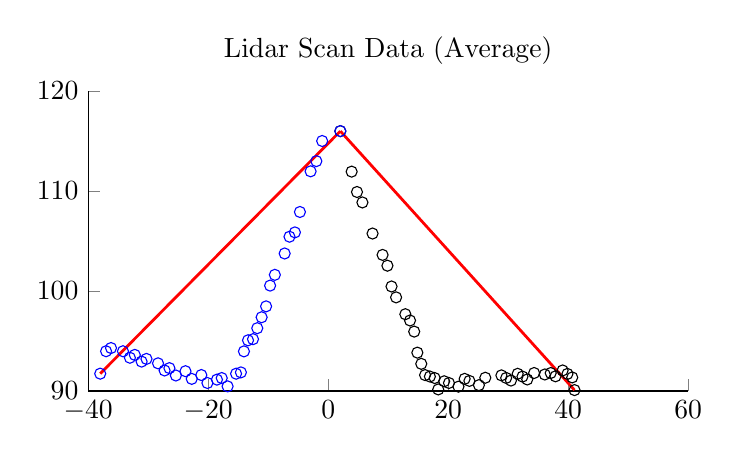
\begin{tikzpicture}

\begin{axis}[%
width=3.0in,
height=1.5in,
unbounded coords=jump,
scale only axis,
xmin=-40,
xmax=60,
ymin=90,
ymax=120,
title={Lidar Scan Data (Average)},
axis x line*=bottom,
axis y line*=left
]
\addplot [
color=black,
only marks,
mark=o,
mark options={solid},
forget plot
]
table[row sep=crcr]{
41.05463 90.08617\\
40.67366 91.35455\\
39.87491 91.70601\\
39.07311 92.05049\\
37.88566 91.46407\\
37.08605 91.7912000000001\\
36.10037 91.64613\\
34.32032 91.79387\\
33.17595 91.15018\\
32.37927 91.43622\\
31.58011 91.7153\\
30.46125 91.03907\\
29.66563 91.30143\\
28.86776 91.55683\\
26.18555 91.31986\\
25.12041 90.58126\\
23.53572 91.00588\\
22.74066 91.2078\\
21.71042 90.4304\\
20.12888 90.79553\\
19.33579 90.96773\\
18.34185 90.15307\\
17.74524 91.29133\\
16.9479 91.44271\\
16.14928 91.58712\\
15.51447 92.71085\\
14.86127 93.83039\\
14.33751 95.93454\\
13.63896 97.04627\\
12.8590803448276 97.6744137931034\\
11.32032 99.35719\\
10.55737 100.4467\\
9.87211300000001 102.5258\\
9.06419700000001 103.6042\\
7.394186 105.7418\\
5.704619 108.8506\\
4.798133 109.8953\\
3.908744 111.9318\\
2.024479 115.9823\\
};
\addplot [
color=blue,
only marks,
mark=o,
mark options={solid},
forget plot
]
table[row sep=crcr]{
2.024479 115.9823\\
};
\addplot [
color=blue,
only marks,
mark=o,
mark options={solid},
forget plot
]
table[row sep=crcr]{
-1.003552 114.9956\\
-1.972122 112.9828\\
-2.931818 111.9616\\
-4.710894 107.8972\\
-5.547611 105.8547\\
-6.44798886206897 105.423710344828\\
-7.254673 103.7467\\
-8.889886 101.6119\\
-9.680421 100.535\\
-10.34832 98.45767\\
-11.09391 97.3700399999999\\
-11.82133 96.2769800000001\\
-12.53051 95.17871\\
-13.36062 95.06573\\
-14.04189 93.95651\\
-14.54841 91.85502\\
-15.34943 91.7245600000001\\
-16.76567 90.45945\\
-17.74524 91.29133\\
-18.54122 91.133\\
-20.12888 90.79553\\
-21.1454 91.59079\\
-22.74066 91.2078\\
-23.7861 91.97403\\
-25.38765 91.54489\\
-26.46119 92.2811200000001\\
-27.26547 92.04669\\
-28.36006 92.76156\\
-30.28367 93.20354\\
-31.09586 92.93572\\
-32.23125 93.60634\\
-33.04688 93.3215100000001\\
-34.20201 93.96926\\
-36.19516 94.29162\\
-37.01662 93.97217\\
-37.9949971428571 91.7280357142857\\
};
\addplot [
color=red,
solid,
line width=1.0pt,
forget plot
]
table[row sep=crcr]{
41.05463 90.08617\\
2.024479 115.9823\\
};
\addplot [
color=red,
solid,
line width=1.0pt,
forget plot
]
table[row sep=crcr]{
2.024479 115.9823\\
-37.9949971428571 91.7280357142857\\
};
\end{axis}
\end{tikzpicture}%
        \caption{Average data from 30 scans. The lidar is located at the origin.}
    \end{figure}
\end{frame}

\begin{frame}{Line Fitting Segmented Data}
    \begin{figure}
        \centering 
        \input{Images/avg_data_5.tikz}
        \caption{Average data from 30 scans. The lidar is located at the origin.}
    \end{figure}
\end{frame}

\begin{frame}{Line Fitting Segmented Data}
    \begin{figure}
        \centering 
        \input{Images/avg_data_6.tikz}
        \caption{Average data from 30 scans. The lidar is located at the origin.}
    \end{figure}
\end{frame}

\begin{frame}{Line Fitting Segmented Data}
    \begin{figure}
        \centering 
        % This file was created by matlab2tikz v0.4.0.
% Copyright (c) 2008--2013, Nico Schlömer <nico.schloemer@gmail.com>
% All rights reserved.
% 
% The latest updates can be retrieved from
%   http://www.mathworks.com/matlabcentral/fileexchange/22022-matlab2tikz
% where you can also make suggestions and rate matlab2tikz.
% 
% 
% 

% defining custom colors
\definecolor{mycolor1}{rgb}{1,0,1}%

\begin{tikzpicture}

\begin{axis}[%
width=3.0in,
height=1.5in,
unbounded coords=jump,
scale only axis,
xmin=-60,
xmax=60,
ymin=70,
ymax=140,
title={Lidar Scan Data (Average)},
axis x line*=bottom,
axis y line*=left
]
\addplot [
color=black,
only marks,
mark=o,
mark options={solid},
forget plot
]
table[row sep=crcr]{
41.05463 90.08617\\
40.67366 91.35455\\
39.87491 91.70601\\
39.07311 92.05049\\
37.88566 91.46407\\
37.08605 91.7912000000001\\
36.10037 91.64613\\
34.32032 91.79387\\
33.17595 91.15018\\
32.37927 91.43622\\
31.58011 91.7153\\
30.46125 91.03907\\
29.66563 91.30143\\
28.86776 91.55683\\
26.18555 91.31986\\
25.12041 90.58126\\
23.53572 91.00588\\
22.74066 91.2078\\
21.71042 90.4304\\
20.12888 90.79553\\
19.33579 90.96773\\
18.34185 90.15307\\
17.74524 91.29133\\
16.9479 91.44271\\
16.14928 91.58712\\
};
\addplot [
color=mycolor1,
only marks,
mark=o,
mark options={solid},
forget plot
]
table[row sep=crcr]{
16.14928 91.58712\\
15.51447 92.71085\\
14.86127 93.83039\\
14.33751 95.93454\\
13.63896 97.04627\\
12.8590803448276 97.6744137931034\\
11.32032 99.35719\\
10.55737 100.4467\\
9.87211300000001 102.5258\\
9.06419700000001 103.6042\\
7.394186 105.7418\\
5.704619 108.8506\\
4.798133 109.8953\\
3.908744 111.9318\\
2.024479 115.9823\\
};
\addplot [
color=blue,
only marks,
mark=o,
mark options={solid},
forget plot
]
table[row sep=crcr]{
2.024479 115.9823\\
};
\addplot [
color=blue,
only marks,
mark=o,
mark options={solid},
forget plot
]
table[row sep=crcr]{
-1.003552 114.9956\\
-1.972122 112.9828\\
-2.931818 111.9616\\
-4.710894 107.8972\\
-5.547611 105.8547\\
-6.44798886206897 105.423710344828\\
-7.254673 103.7467\\
-8.889886 101.6119\\
-9.680421 100.535\\
-10.34832 98.45767\\
-11.09391 97.3700399999999\\
-11.82133 96.2769800000001\\
-12.53051 95.17871\\
-13.36062 95.06573\\
-14.04189 93.95651\\
-14.54841 91.85502\\
-15.34943 91.7245600000001\\
-16.76567 90.45945\\
};
\addplot [
color=green,
only marks,
mark=o,
mark options={solid},
forget plot
]
table[row sep=crcr]{
-16.76567 90.45945\\
-17.74524 91.29133\\
-18.54122 91.133\\
-20.12888 90.79553\\
-21.1454 91.59079\\
-22.74066 91.2078\\
-23.7861 91.97403\\
-25.38765 91.54489\\
-26.46119 92.2811200000001\\
-27.26547 92.04669\\
-28.36006 92.76156\\
-30.28367 93.20354\\
-31.09586 92.93572\\
-32.23125 93.60634\\
-33.04688 93.3215100000001\\
-34.20201 93.96926\\
-36.19516 94.29162\\
-37.01662 93.97217\\
-37.9949971428571 91.7280357142857\\
};
\addplot [
color=red,
solid,
line width=1.0pt,
forget plot
]
table[row sep=crcr]{
6.14928 90.6010844453305\\
7.14928 90.6318897325013\\
8.14928 90.662695019672\\
9.14928 90.6935003068428\\
10.14928 90.7243055940135\\
11.14928 90.7551108811842\\
12.14928 90.785916168355\\
13.14928 90.8167214555257\\
14.14928 90.8475267426965\\
15.14928 90.8783320298672\\
16.14928 90.909137317038\\
17.14928 90.9399426042087\\
18.14928 90.9707478913795\\
19.14928 91.0015531785502\\
20.14928 91.032358465721\\
21.14928 91.0631637528917\\
22.14928 91.0939690400625\\
23.14928 91.1247743272332\\
24.14928 91.155579614404\\
25.14928 91.1863849015747\\
26.14928 91.2171901887454\\
27.14928 91.2479954759162\\
28.14928 91.2788007630869\\
29.14928 91.3096060502577\\
30.14928 91.3404113374284\\
31.14928 91.3712166245992\\
32.14928 91.4020219117699\\
33.14928 91.4328271989407\\
34.14928 91.4636324861114\\
35.14928 91.4944377732822\\
36.14928 91.5252430604529\\
37.14928 91.5560483476237\\
38.14928 91.5868536347944\\
39.14928 91.6176589219652\\
40.14928 91.6484642091359\\
41.14928 91.6792694963067\\
42.14928 91.7100747834774\\
43.14928 91.7408800706482\\
44.14928 91.7716853578189\\
45.14928 91.8024906449896\\
46.14928 91.8332959321604\\
47.14928 91.8641012193311\\
48.14928 91.8949065065019\\
49.14928 91.9257117936726\\
50.14928 91.9565170808434\\
};
\addplot [
color=red,
solid,
line width=1.0pt,
forget plot
]
table[row sep=crcr]{
-7.975521 131.500579318584\\
-6.975521 129.858861106927\\
-5.975521 128.21714289527\\
-4.975521 126.575424683612\\
-3.975521 124.933706471955\\
-2.975521 123.291988260298\\
-1.975521 121.650270048641\\
-0.975521000000001 120.008551836983\\
0.0244789999999995 118.366833625326\\
1.024479 116.725115413669\\
2.024479 115.083397202011\\
3.024479 113.441678990354\\
4.024479 111.799960778697\\
5.024479 110.158242567039\\
6.024479 108.516524355382\\
7.024479 106.874806143725\\
8.024479 105.233087932068\\
9.024479 103.59136972041\\
10.024479 101.949651508753\\
11.024479 100.307933297096\\
12.024479 98.6662150854383\\
13.024479 97.024496873781\\
14.024479 95.3827786621237\\
15.024479 93.7410604504664\\
16.024479 92.0993422388091\\
17.024479 90.4576240271518\\
18.024479 88.8159058154945\\
19.024479 87.1741876038372\\
20.024479 85.5324693921799\\
21.024479 83.8907511805226\\
22.024479 82.2490329688654\\
23.024479 80.607314757208\\
24.024479 78.9655965455507\\
25.024479 77.3238783338934\\
26.024479 75.6821601222362\\
};
\addplot [
color=red,
solid,
line width=1.0pt,
forget plot
]
table[row sep=crcr]{
-26.76567 73.0888523708592\\
-25.76567 74.6796915318638\\
-24.76567 76.2705306928684\\
-23.76567 77.861369853873\\
-22.76567 79.4522090148775\\
-21.76567 81.0430481758821\\
-20.76567 82.6338873368867\\
-19.76567 84.2247264978913\\
-18.76567 85.8155656588959\\
-17.76567 87.4064048199004\\
-16.76567 88.997243980905\\
-15.76567 90.5880831419096\\
-14.76567 92.1789223029142\\
-13.76567 93.7697614639188\\
-12.76567 95.3606006249234\\
-11.76567 96.9514397859279\\
-10.76567 98.5422789469325\\
-9.76567 100.133118107937\\
-8.76567 101.723957268942\\
-7.76567 103.314796429946\\
-6.76567 104.905635590951\\
-5.76567 106.496474751955\\
-4.76567 108.08731391296\\
-3.76567 109.678153073965\\
-2.76567 111.268992234969\\
-1.76567 112.859831395974\\
-0.76567 114.450670556978\\
0.23433 116.041509717983\\
1.23433 117.632348878988\\
2.23433 119.223188039992\\
3.23433 120.814027200997\\
4.23433 122.404866362001\\
5.23433 123.995705523006\\
6.23433 125.58654468401\\
7.23433 127.177383845015\\
8.23433 128.76822300602\\
9.23433 130.359062167024\\
10.23433 131.949901328029\\
11.23433 133.540740489033\\
};
\addplot [
color=red,
solid,
line width=1.0pt,
forget plot
]
table[row sep=crcr]{
-47.9949971428571 96.1594644274003\\
-46.9949971428571 95.9800733176636\\
-45.9949971428571 95.800682207927\\
-44.9949971428571 95.6212910981903\\
-43.9949971428571 95.4418999884536\\
-42.9949971428571 95.262508878717\\
-41.9949971428571 95.0831177689803\\
-40.9949971428571 94.9037266592436\\
-39.9949971428571 94.724335549507\\
-38.9949971428571 94.5449444397703\\
-37.9949971428571 94.3655533300336\\
-36.9949971428571 94.186162220297\\
-35.9949971428571 94.0067711105603\\
-34.9949971428571 93.8273800008237\\
-33.9949971428571 93.647988891087\\
-32.9949971428571 93.4685977813503\\
-31.9949971428571 93.2892066716137\\
-30.9949971428571 93.109815561877\\
-29.9949971428571 92.9304244521403\\
-28.9949971428571 92.7510333424037\\
-27.9949971428571 92.571642232667\\
-26.9949971428571 92.3922511229303\\
-25.9949971428571 92.2128600131937\\
-24.9949971428571 92.033468903457\\
-23.9949971428571 91.8540777937204\\
-22.9949971428571 91.6746866839837\\
-21.9949971428571 91.495295574247\\
-20.9949971428571 91.3159044645104\\
-19.9949971428571 91.1365133547737\\
-18.9949971428571 90.957122245037\\
-17.9949971428571 90.7777311353004\\
-16.9949971428571 90.5983400255637\\
-15.9949971428571 90.418948915827\\
-14.9949971428571 90.2395578060904\\
-13.9949971428571 90.0601666963537\\
-12.9949971428571 89.880775586617\\
-11.9949971428571 89.7013844768804\\
-10.9949971428571 89.5219933671437\\
-9.99499714285714 89.3426022574071\\
-8.99499714285714 89.1632111476704\\
-7.99499714285714 88.9838200379337\\
-6.99499714285714 88.8044289281971\\
};
\end{axis}
\end{tikzpicture}%
        \caption{Average data from 30 scans. The lidar is located at the origin.}
    \end{figure}
\end{frame}

\begin{frame}{Line Fitting Segmented Data}
    \begin{figure}
        \centering 
        \input{Images/avg_data_8.tikz}
        \caption{Average data from 30 scans. The lidar is located at the origin.}
    \end{figure}
\end{frame}

\begin{frame}{Calculating Target Apex}
    \begin{figure}
        \centering 
        \includegraphics[height=.55\textwidth]{Images/circle.png}
        \caption{Determine the position of the apex by calculating distances between each base intersection point ($b_{0}, b_{1}, b_{2}$) and the distance from each base point to the target apex ($s_{0}, s_{1}, s_{2}$)}
    \end{figure}
% describe localization of apex using triangulation
% note that this is only possible because of target construction
\end{frame}

\begin{frame}{Optimal Transformation Between Two Lidars}
    \[
    \Sigma^2 = \displaystyle\sum\limits_{i=1}^n {\parallel \hat{x}_i - ({\Omega}x_i + \tau) \parallel^2} \]
    \begin{figure}
        \centering
        % This file was created by matlab2tikz v0.4.0.
% Copyright (c) 2008--2013, Nico Schlömer <nico.schloemer@gmail.com>
% All rights reserved.
% 
% The latest updates can be retrieved from
%   http://www.mathworks.com/matlabcentral/fileexchange/22022-matlab2tikz
% where you can also make suggestions and rate matlab2tikz.
% 
% 
% 
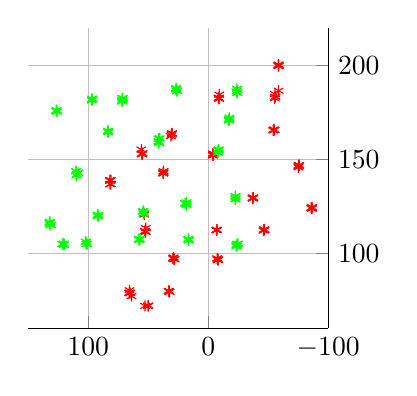
\begin{tikzpicture}

\begin{axis}[%
width=1.5in,
height=1.5in,
view={-90}{90},
scale only axis,
xmin=60,
xmax=220,
xmajorgrids,
ymin=-100,
ymax=150,
ymajorgrids,
zmin=0,
zmax=20,
zmajorgrids,
axis x line*=bottom,
axis y line*=left,
axis z line*=left
]
\addplot3 [
color=red,
only marks,
mark=asterisk,
mark options={solid}]
table[row sep=crcr] {
71.81076 50.11689 9.728381\\
72.09412 49.86405 9.880158\\
72.0287 50.06058 9.857063\\
71.90044 52.65413 9.356509\\
77.09086 63.9604 7.221591e-16\\
78.68705 65.61092 8.449825\\
78.88257 65.74714 8.492682\\
80.25962 65.62736 8.157181\\
79.0022 65.71169 8.585256\\
78.85325 65.06079 8.561256\\
111.3033 52.04466 9.953863\\
113.3979 52.06614 9.214791\\
111.729 52.67679 9.727344\\
120.6257 53.27854 3.891204e-16\\
111.864 52.6995 10.03056\\
143.052 37.44499 11.69009\\
142.4563 37.46961 11.43347\\
142.7963 37.40165 11.31265\\
143.8084 37.17722 11.41399\\
143.062 37.31889 11.58954\\
152.1632 -3.950336 13.92609\\
152.1898 -3.960711 14.04684\\
153.1695 -3.867313 13.57368\\
153.12 -4.107715 13.49174\\
152.4689 -4.472018 13.89954\\
166.0073 -54.85455 15.86172\\
165.5409 -54.15384 16.22846\\
165.6192 -54.48528 16.22889\\
165.7002 -55.35326 16.16767\\
165.7171 -54.50734 16.38244\\
186.693 -58.70256 15.74962\\
183.4777 -55.98117 17.61618\\
183.3008 -55.86508 17.20183\\
184.8777 -55.66872 17.05019\\
182.5921 -55.38595 17.5461\\
200.3777 -58.71131 17.17585\\
199.8373 -58.54858 17.77914\\
199.8603 -58.59904 17.73903\\
200.6078 -58.56987 17.23171\\
200.4706 -58.4629 17.38979\\
182.8517 -8.9787 14.17156\\
182.3662 -9.099507 14.49154\\
182.6465 -8.911176 14.20983\\
182.8583 -8.600733 14.13756\\
184.5445 -9.205479 14.08374\\
162.4429 31.09821 11.37109\\
163.8818 30.23875 11.75643\\
163.844 30.24096 11.68944\\
163.1778 30.64583 11.42419\\
163.7927 30.11347 11.74713\\
153.0106 55.18719 11.02093\\
152.9578 55.51322 10.57525\\
152.7426 55.06438 10.63689\\
155.2766 55.75882 10.31159\\
153.3297 54.78237 10.62594\\
79.85257 32.8998 10.69603\\
79.38042 32.2171 10.63294\\
79.84695 32.80175 10.84837\\
79.7178 32.5711 10.7691\\
79.80017 32.94861 10.68066\\
138.9018 81.04651 8.506819\\
136.9132 81.08249 8.899706\\
139.0158 81.98875 8.070492\\
138.6356 81.91949 8.155473\\
136.8475 81.82059 8.697878\\
96.33623 -8.185828 13.41041\\
97.28129 -7.459514 13.20078\\
96.60412 -8.261885 13.52678\\
96.89125 -7.947184 13.55592\\
96.65429 -7.580743 13.57671\\
112.7264 -46.75028 16.11029\\
112.0596 -46.06171 16.30243\\
112.4381 -46.91394 16.1783\\
112.4863 -46.23947 16.07938\\
112.3708 -46.59448 16.21878\\
123.9022 -86.44815 17.6398\\
123.7415 -86.16577 17.79677\\
124.2774 -85.72666 17.52168\\
124.2606 -86.21016 17.63495\\
124.5722 -86.60898 17.54244\\
129.6249 -37.43633 15.28435\\
129.7241 -37.61682 15.1838\\
129.152 -37.13404 15.3966\\
129.3599 -37.42214 15.24854\\
129.4794 -36.86441 15.11455\\
146.9347 -75.6037 17.35716\\
146.3593 -75.44043 17.50633\\
146.7223 -75.08581 17.25374\\
145.7984 -75.09916 17.57354\\
146.9577 -75.84589 17.21411\\
112.5186 -7.340799 14.0963\\
112.2783 -6.990843 13.94974\\
112.3847 -7.042787 13.92603\\
112.3563 -6.828396 13.83346\\
112.4431 -6.99584 13.99827\\
96.82921 27.99927 11.80589\\
97.2145 29.34815 11.52174\\
96.80501 28.48206 11.42314\\
97.42975 29.20447 11.52999\\
97.75054 28.87651 11.53954\\
};
\addplot3 [
color=green,
only marks,
mark=asterisk,
mark options={solid}]
table[row sep=crcr] {
104.5648 120.0087 12.80935\\
104.6622 120.8717 12.67868\\
105.1877 120.4338 12.50175\\
104.9624 121.7491 12.75633\\
104.6827 120.8198 12.75878\\
116.6436 132.3991 12.09633\\
116.0964 131.9448 12.3467\\
115.3698 132.231 12.30791\\
116.6669 131.818 12.30196\\
115.0085 131.0785 12.52533\\
143.7626 110.3246 10.58592\\
142.8974 108.375 12.23887\\
143.6858 109.9591 11.54597\\
142.2536 109.3907 11.54246\\
141.4563 109.9516 11.57257\\
165.0799 83.43453 11.67853\\
164.4613 83.18241 12.13538\\
164.988 83.2346 12.12438\\
164.9352 83.59583 11.71528\\
165.3189 83.58157 11.59992\\
161.2878 40.37335 11.96013\\
161.0845 41.53905 12.18813\\
159.2355 41.2131 12.5195\\
158.7147 41.08862 12.49865\\
159.7389 41.38341 12.34793\\
154.8751 -8.006658 12.3167\\
154.8549 -8.721751 12.22706\\
155.3744 -8.718247 12.20826\\
153.6771 -8.282025 12.49871\\
153.7382 -8.065492 12.39661\\
172.3058 -17.66948 12.24947\\
171.2848 -17.47856 12.17522\\
171.3599 -16.89454 12.17049\\
171.6551 -17.66995 11.99852\\
170.7352 -17.05774 12.41018\\
185.5108 -24.24228 12.61854\\
186.9695 -24.42205 12.20739\\
187.717 -23.85406 11.76797\\
186.283 -23.54275 12.07451\\
185.5745 -24.21254 12.57785\\
186.5677 25.89911 11.63176\\
186.4571 26.31884 11.85219\\
188.1206 26.718 11.17391\\
187.3095 26.39343 11.65014\\
187.5168 27.04277 11.21782\\
181.3122 71.67948 11.00632\\
180.8698 71.95046 11.06199\\
181.7721 71.58231 11.29755\\
182.7011 71.1322 10.9436\\
182.6706 71.72332 11.00347\\
182.4425 96.73309 11.11435\\
182.0726 96.6987 11.5778\\
182.1495 96.85112 11.19854\\
181.4532 97.01761 11.1384\\
182.2018 96.42782 11.09595\\
106.2032 102.2265 12.9082\\
104.9459 101.506 13.26096\\
104.9602 100.7852 13.11163\\
105.8522 101.7037 13.02191\\
104.9097 101.4066 13.2517\\
175.9253 126.7314 11.322\\
176.2417 126.4086 11.14123\\
176.1857 126.3554 11.04248\\
176.1279 126.3783 11.1444\\
175.4093 126.039 11.38325\\
107.2624 57.58489 13.45017\\
107.4651 57.83386 13.28392\\
106.9868 57.50553 13.32428\\
107.643 57.34066 13.31998\\
107.4967 56.84323 13.18608\\
106.9328 16.34695 13.5584\\
107.5071 16.37696 13.44934\\
107.5365 16.53915 13.80174\\
107.5967 16.69866 13.84571\\
106.8634 16.07849 13.61015\\
105.1318 -24.85122 13.87729\\
103.5312 -23.28218 14.00363\\
104.0334 -24.12825 13.93625\\
104.3003 -23.39779 13.79684\\
104.8211 -23.98417 13.82746\\
126.533 19.20647 12.92298\\
125.6681 18.17298 13.24934\\
126.3211 18.36944 13.1773\\
127.1731 18.05003 13.13356\\
126.683 19.20479 12.97892\\
130.4268 -22.80068 13.17138\\
130.4504 -22.58967 12.92274\\
128.8032 -22.54907 13.22447\\
129.725 -22.73897 13.04894\\
128.8792 -22.74695 13.18723\\
122.3884 53.95481 12.99149\\
121.3962 53.50307 13.25203\\
122.3686 54.50889 13.15496\\
122.253 53.87533 12.80835\\
121.1066 54.1042 13.26104\\
120.1549 91.48139 12.46721\\
119.595 91.87903 12.93271\\
120.2082 92.3701 12.80872\\
120.3168 92.35238 12.79442\\
120.5105 91.93338 12.58505\\
};
\end{axis}
\end{tikzpicture}%
    \end{figure}
\end{frame}

\begin{frame}{Optimal Transformation Between Two Lidars}
    \[
    \Sigma^2 = \displaystyle\sum\limits_{i=1}^n {\parallel \hat{x}_i - ({\Omega}x_i + \tau) \parallel^2} \]
    \begin{figure}
        \centering
        % This file was created by matlab2tikz v0.4.0.
% Copyright (c) 2008--2013, Nico Schlömer <nico.schloemer@gmail.com>
% All rights reserved.
% 
% The latest updates can be retrieved from
%   http://www.mathworks.com/matlabcentral/fileexchange/22022-matlab2tikz
% where you can also make suggestions and rate matlab2tikz.
% 
% 
% 
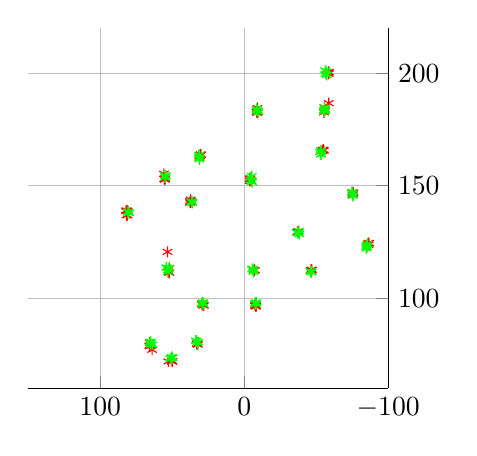
\begin{tikzpicture}

\begin{axis}[%
width=1.8in,
height=1.8in,
view={-90}{90},
scale only axis,
xmin=60,
xmax=220,
xmajorgrids,
ymin=-100,
ymax=150,
ymajorgrids,
zmin=0,
zmax=20,
zmajorgrids,
axis x line*=bottom,
axis y line*=left,
axis z line*=left
]
\addplot3 [
color=red,
only marks,
mark=asterisk,
mark options={solid}]
table[row sep=crcr] {
71.81076 50.11689 9.728381\\
72.09412 49.86405 9.880158\\
72.0287 50.06058 9.857063\\
71.90044 52.65413 9.356509\\
77.09086 63.9604 7.221591e-16\\
78.68705 65.61092 8.449825\\
78.88257 65.74714 8.492682\\
80.25962 65.62736 8.157181\\
79.0022 65.71169 8.585256\\
78.85325 65.06079 8.561256\\
111.3033 52.04466 9.953863\\
113.3979 52.06614 9.214791\\
111.729 52.67679 9.727344\\
120.6257 53.27854 3.891204e-16\\
111.864 52.6995 10.03056\\
143.052 37.44499 11.69009\\
142.4563 37.46961 11.43347\\
142.7963 37.40165 11.31265\\
143.8084 37.17722 11.41399\\
143.062 37.31889 11.58954\\
152.1632 -3.950336 13.92609\\
152.1898 -3.960711 14.04684\\
153.1695 -3.867313 13.57368\\
153.12 -4.107715 13.49174\\
152.4689 -4.472018 13.89954\\
166.0073 -54.85455 15.86172\\
165.5409 -54.15384 16.22846\\
165.6192 -54.48528 16.22889\\
165.7002 -55.35326 16.16767\\
165.7171 -54.50734 16.38244\\
186.693 -58.70256 15.74962\\
183.4777 -55.98117 17.61618\\
183.3008 -55.86508 17.20183\\
184.8777 -55.66872 17.05019\\
182.5921 -55.38595 17.5461\\
200.3777 -58.71131 17.17585\\
199.8373 -58.54858 17.77914\\
199.8603 -58.59904 17.73903\\
200.6078 -58.56987 17.23171\\
200.4706 -58.4629 17.38979\\
182.8517 -8.9787 14.17156\\
182.3662 -9.099507 14.49154\\
182.6465 -8.911176 14.20983\\
182.8583 -8.600733 14.13756\\
184.5445 -9.205479 14.08374\\
162.4429 31.09821 11.37109\\
163.8818 30.23875 11.75643\\
163.844 30.24096 11.68944\\
163.1778 30.64583 11.42419\\
163.7927 30.11347 11.74713\\
153.0106 55.18719 11.02093\\
152.9578 55.51322 10.57525\\
152.7426 55.06438 10.63689\\
155.2766 55.75882 10.31159\\
153.3297 54.78237 10.62594\\
79.85257 32.8998 10.69603\\
79.38042 32.2171 10.63294\\
79.84695 32.80175 10.84837\\
79.7178 32.5711 10.7691\\
79.80017 32.94861 10.68066\\
138.9018 81.04651 8.506819\\
136.9132 81.08249 8.899706\\
139.0158 81.98875 8.070492\\
138.6356 81.91949 8.155473\\
136.8475 81.82059 8.697878\\
96.33623 -8.185828 13.41041\\
97.28129 -7.459514 13.20078\\
96.60412 -8.261885 13.52678\\
96.89125 -7.947184 13.55592\\
96.65429 -7.580743 13.57671\\
112.7264 -46.75028 16.11029\\
112.0596 -46.06171 16.30243\\
112.4381 -46.91394 16.1783\\
112.4863 -46.23947 16.07938\\
112.3708 -46.59448 16.21878\\
123.9022 -86.44815 17.6398\\
123.7415 -86.16577 17.79677\\
124.2774 -85.72666 17.52168\\
124.2606 -86.21016 17.63495\\
124.5722 -86.60898 17.54244\\
129.6249 -37.43633 15.28435\\
129.7241 -37.61682 15.1838\\
129.152 -37.13404 15.3966\\
129.3599 -37.42214 15.24854\\
129.4794 -36.86441 15.11455\\
146.9347 -75.6037 17.35716\\
146.3593 -75.44043 17.50633\\
146.7223 -75.08581 17.25374\\
145.7984 -75.09916 17.57354\\
146.9577 -75.84589 17.21411\\
112.5186 -7.340799 14.0963\\
112.2783 -6.990843 13.94974\\
112.3847 -7.042787 13.92603\\
112.3563 -6.828396 13.83346\\
112.4431 -6.99584 13.99827\\
96.82921 27.99927 11.80589\\
97.2145 29.34815 11.52174\\
96.80501 28.48206 11.42314\\
97.42975 29.20447 11.52999\\
97.75054 28.87651 11.53954\\
};
\addplot3 [
color=green,
only marks,
mark=asterisk,
mark options={solid}]
table[row sep=crcr] {
73.4621881637701 49.7082807848115 9.22756586923505\\
73.2591407804359 50.5447433216751 9.05311646841991\\
73.9094988119042 50.3094979926788 8.90853102312862\\
73.2340939262325 51.4742810904186 9.0893451045228\\
73.2935864610403 50.5067568064726 9.13618505303808\\
80.5200337380405 65.480535898635 8.06541114863221\\
80.1557648827262 64.8757779851728 8.33013276477407\\
79.3767977464519 64.8896148547769 8.26394057683402\\
80.7360531759212 64.9533379181521 8.30184652824465\\
79.4297121595747 63.6940656070406 8.53583661858726\\
113.639937359923 54.1640523855218 8.18471996105735\\
113.447265514129 52.1095032164052 9.92352994895723\\
113.661600645003 53.8369702626871 9.16131224010808\\
112.515850328404 52.8066601801795 9.16356301693796\\
111.573117573053 53.0562306783638 9.15043935417833\\
142.899038319356 36.4344404143667 11.0592305115713\\
142.39074482111 36.0032596538734 11.5182111738233\\
142.866833670002 36.2347202241129 11.5134050854577\\
142.706267084023 36.5368349684426 11.0849394326621\\
143.074879305243 36.6517948982476 10.9770218154421\\
154.245442400078 -5.2040582298824 13.5530406591661\\
153.643376832316 -4.17291176557483 13.7155995754465\\
152.011442520296 -5.10636137735433 14.0323213822716\\
151.567008948491 -5.40487286946606 14.0092492729084\\
152.430287824869 -4.77937950683713 13.8605518035042\\
164.974247083268 -52.7319157955541 16.3584894329183\\
165.206002929025 -53.4126384197991 16.3064576633198\\
165.692467970707 -53.2296223682728 16.2963158626466\\
163.940231658945 -53.3982547993192 16.5344526651914\\
163.926031474202 -53.1786671344884 16.4220971032621\\
184.663958079798 -55.7272892328486 17.0980637772867\\
183.643197973555 -55.9065656022099 16.996509369257\\
183.511533052435 -55.3336541543954 16.9621791375416\\
184.062686103447 -55.9648504526464 16.8364853173495\\
182.974171796373 -55.6931584069595 17.1995295092948\\
199.307091067215 -57.2780275910259 18.0381724743098\\
200.750971115012 -56.9573932083414 17.6619129021872\\
201.270132693316 -56.1847942025015 17.20581986531\\
199.807444543184 -56.3782095238854 17.4710943959705\\
199.357906297369 -57.2298106326117 17.9970534883585\\
182.968862671033 -9.98937055232069 14.4194749378411\\
182.712276810935 -9.62504193639145 14.615493747685\\
184.156841476854 -8.70265187681665 13.9453786695252\\
183.492501898696 -9.2677499783745 14.4242742409283\\
183.476809900292 -8.60639503600552 13.9618029343695\\
162.210469493268 31.0364539182557 11.285057612844\\
161.699974621795 31.1389383813466 11.3188065435746\\
162.665295661239 31.1180079621472 11.5887795690033\\
163.704231755696 31.0038298770677 11.2749392097076\\
163.468893813938 31.5495123961629 11.3029421171117\\
154.590898354302 54.9002376298205 10.0873158923974\\
154.240141036427 54.7597172549898 10.5455930059588\\
154.272452747767 54.912634166644 10.1601633944336\\
153.564076721622 54.8239438394289 10.079498277176\\
154.471579844229 54.5298485710087 10.0810023223803\\
81.1524066483528 33.626512303749 10.2943483697422\\
80.2110855761111 32.5300951372133 10.6633296612457\\
80.4792071663474 31.8534094736233 10.552587147093\\
81.0004798407102 33.0198133474051 10.4295719830304\\
80.2118853210013 32.4240069073957 10.65872580392\\
138.086095419412 80.7418415590398 8.59781810307451\\
138.500695964843 80.541561666793 8.43976448751956\\
138.470001869223 80.4679540682963 8.34302981722174\\
138.404391443635 80.4737680630713 8.44260092708281\\
137.840006884064 79.9166492008511 8.686831176593\\
97.5852775901916 -7.79480237819213 13.2140096756948\\
97.6947943826274 -7.49842214145437 13.0382904654591\\
97.3586960260482 -7.97042184947549 13.0878341717471\\
98.0311254840014 -7.89696707631404 13.1033926831345\\
98.0708066240487 -8.41957871297248 12.9935200784792\\
111.552386821956 -46.5297426646559 15.4970572110173\\
112.084141936226 -46.3067981100408 15.39632291837\\
112.043464820581 -46.1292671021614 15.7401016693191\\
112.043160875486 -45.9570193143049 15.7765906840485\\
111.578512431829 -46.8030521598322 15.5617454360294\\
124.119059545825 -85.7296219432653 17.9633711356059\\
122.070833368621 -84.8107739835444 17.9793908463366\\
122.836933791027 -85.4316387237149 17.965374195425\\
122.838988895067 -84.6607895864285 17.7920826670911\\
123.529243320946 -85.0276712649294 17.8624985057545\\
128.959267805117 -37.0669913425803 15.0439732216236\\
128.495110405792 -38.3213400138213 15.4098034545293\\
129.04174043131 -37.9135212940773 15.3385658224256\\
129.952599000035 -37.9184867987385 15.326239134098\\
129.09855830463 -37.0139869636749 15.1024608148571\\
147.147395256983 -75.0484095523176 17.5793080504416\\
147.104973074727 -74.853431819074 17.3202943988867\\
145.536314692059 -75.3747142534155 17.5914635251395\\
146.472281068903 -75.2398749904438 17.4418863026836\\
145.677362964807 -75.5352696498746 17.5660339867521\\
113.038724649121 -5.95778570494471 13.2046348217993\\
112.256030832167 -6.71436403983743 13.4718249624718\\
112.822693781474 -5.43855037791404 13.3382180044501\\
112.945584885221 -6.08729186457041 13.0236828143508\\
111.77606194343 -6.25158011136193 13.4441208402145\\
97.9681180418854 28.3919428379316 10.6589396740134\\
97.2895616343872 28.5901330090389 11.0931949992768\\
97.6986421125608 29.2577924608888 10.9538338722262\\
97.8070813359362 29.2783149470296 10.9423355768599\\
98.1409420929475 28.9440353205831 10.7587310748165\\
};
\end{axis}
\end{tikzpicture}%
    \end{figure}
\end{frame}

% --------------------------------------------------- Results --------------------------------------------------- %

\section{Verification}

\subsection{Experimental Results}
\begin{frame}{Full 6DoF Transformation between Lidars}
    \begin{figure}
    \vskip-80pt
        \includegraphics<1>[width=1\textwidth]{Images/6dof_rot.pdf}
        \includegraphics<2>[width=1\textwidth]{Images/6dof_trans.pdf}
    \end{figure}
\end{frame}


\begin{frame}{Total Error Across All Transformations}
    \begin{figure}
        \centering
        \includegraphics[width=.9\textwidth]{Images/total_error.jpg}
    \end{figure}
\end{frame}

\begin{frame}{Human Error in Hand Calibration}
    \begin{figure}
        \centering
        \input{Images/hand_calibrate_1.tikz}
    \end{figure}
\end{frame}

\begin{frame}{Human Error in Hand Calibration}
    \begin{figure}
        \centering
        % This file was created by matlab2tikz v0.4.0.
% Copyright (c) 2008--2013, Nico Schlömer <nico.schloemer@gmail.com>
% All rights reserved.
% 
% The latest updates can be retrieved from
%   http://www.mathworks.com/matlabcentral/fileexchange/22022-matlab2tikz
% where you can also make suggestions and rate matlab2tikz.
% 
% 
% 
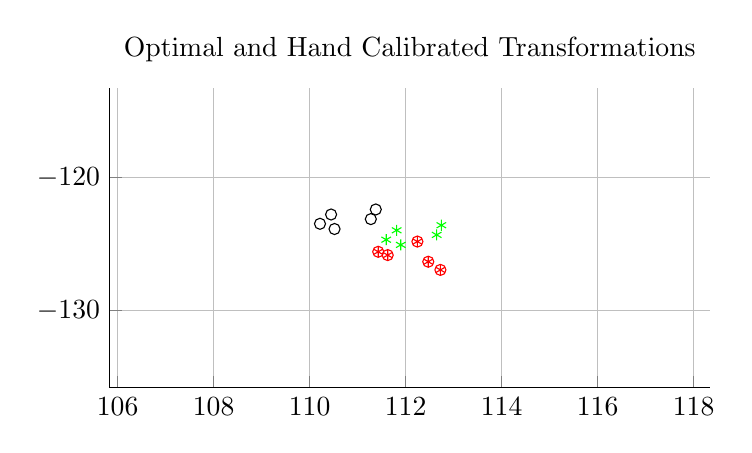
\begin{tikzpicture}

\begin{axis}[%
width=3.0in,
height=1.5in,
view={-0}{90},
scale only axis,
xmin=105.835253456221,
xmax=118.335253456221,
xmajorgrids,
ymin=-135.790857511878,
ymax=-113.290857511878,
ymajorgrids,
zmin=10,
zmax=14,
zmajorgrids,
title={Optimal and Hand Calibrated Transformations},
axis x line*=bottom,
axis y line*=left,
axis z line*=left
]
\addplot3 [
color=red,
only marks,
mark=asterisk,
mark options={solid}]
table[row sep=crcr] {
87.35643 19.88319 12.92156\\
86.62446 18.87714 13.02438\\
86.15504 19.81685 12.94128\\
86.54701 18.48541 13.11535\\
87.02429 19.21749 13.03264\\
98.1544 30.85553 11.87828\\
98.00201 30.54874 12.02612\\
98.20429 30.82365 12.34854\\
97.68108 30.20432 12.21287\\
98.39615 30.29112 12.08218\\
123.2942 6.707566 12.16518\\
123.5707 7.091899 12.07615\\
122.7501 7.102009 12.16326\\
123.2667 7.563118 12.13414\\
122.8061 7.452347 12.11949\\
146.0347 -15.10226 11.38974\\
145.1148 -15.55521 11.51163\\
145.321 -15.99108 11.44012\\
145.8237 -15.38647 11.30412\\
145.0836 -15.29791 11.61078\\
143.2752 -60.53436 11.11841\\
143.0138 -60.47371 11.1937\\
142.3696 -60.1796 11.18904\\
142.652 -60.15351 11.06276\\
142.9805 -60.69332 10.89302\\
134.9616 -116.5097 11.45747\\
135.1301 -116.1073 11.57322\\
135.4623 -115.5045 11.33882\\
135.159 -115.9649 11.48146\\
134.865 -116.4466 11.41041\\
154.1923 -114.8297 10.59426\\
154.4665 -115.5396 10.59905\\
154.0654 -115.2085 10.61656\\
154.2002 -115.7273 10.74194\\
153.8662 -115.6108 10.69978\\
169.7202 -127.7685 10.25302\\
169.5566 -127.5083 10.09834\\
169.4023 -127.2668 10.00832\\
170.131 -128.3399 10.13421\\
169.9424 -128.2696 10.13125\\
168.8233 -75.33921 10.27299\\
168.9328 -74.50341 10.35557\\
168.4501 -75.46583 10.70285\\
168.4295 -75.48979 10.62608\\
168.6088 -75.42636 10.34381\\
162.5836 -31.25825 10.56203\\
162.7785 -31.11936 10.57871\\
163.2288 -31.08736 10.82379\\
162.8885 -31.37783 10.81321\\
162.3081 -31.73278 10.79958\\
162.5587 -4.697574 10.92966\\
162.4932 -4.659549 10.91124\\
162.8115 -4.693533 10.69749\\
162.5564 -4.787738 10.64702\\
162.0269 -4.251013 10.80635\\
87.01635 -1.335527 13.5202\\
86.25722 -1.222405 13.14969\\
86.31634 -1.038465 13.34368\\
86.90447 -1.051315 13.27287\\
85.99736 -0.8786618 13.18766\\
157.0602 26.24962 11.51273\\
160.8208 25.30365 8.802854\\
156.5061 27.00409 11.29012\\
157.2623 26.62164 11.10635\\
156.2641 26.80535 11.13804\\
88.59854 -45.4312 12.87889\\
89.46996 -46.03986 13.38143\\
88.35704 -46.05662 13.22232\\
88.26899 -46.28865 13.06917\\
88.37295 -45.92236 13.17023\\
90.44178 -82.56598 12.80802\\
90.37685 -82.22468 12.65211\\
90.05482 -82.81255 12.72222\\
89.96015 -83.25623 12.73825\\
89.76072 -82.05141 12.63651\\
88.59764 -123.8561 12.55027\\
88.1517 -124.3668 12.30429\\
88.48324 -123.6832 12.51233\\
88.38786 -123.9907 12.49359\\
88.08263 -123.3986 12.52068\\
111.6264 -125.8324 11.66588\\
112.245 -124.8177 11.35906\\
112.4715 -126.3295 11.79512\\
112.7244 -126.9427 10.88207\\
111.4285 -125.5842 11.63105\\
110.2094 -80.45269 12.02134\\
109.5415 -80.72644 12.07301\\
109.6883 -80.06627 12.06187\\
109.9549 -80.44942 11.84295\\
109.6675 -80.22642 12.03372\\
103.5844 -44.47134 13.02523\\
104.2531 -44.78387 12.98159\\
103.6074 -44.36655 13.11734\\
104.9995 -45.43048 12.75167\\
103.7257 -43.98762 13.12165\\
100.505 -5.222584 12.51149\\
100.6828 -5.109821 12.49002\\
100.7231 -4.903094 12.64929\\
100.5587 -5.110365 12.54244\\
100.6838 -4.773956 12.45894\\
};
\addplot3 [
color=green,
only marks,
mark=asterisk,
mark options={solid}]
table[row sep=crcr] {
87.5026793667733 17.9649348761182 12.9337057039736\\
87.0950475821441 19.0612610040921 12.6115129174594\\
87.0010562366618 18.5568953988219 12.8248739921541\\
87.0803574172674 18.2148670621435 12.9064986340435\\
86.4832194162365 18.3039759210598 12.8405614132389\\
96.8419342923573 29.8485617215411 12.8569679838016\\
96.7715191237262 29.983828808929 12.7996835182261\\
97.7244687412745 29.217255325153 12.5112630071903\\
97.6529620176717 29.4449393645121 12.5475931558377\\
96.9161025586528 30.2171173623558 12.5819230174808\\
123.470455816189 5.788565055753 11.8592777799268\\
123.46787454427 6.26757055277339 11.7280123870789\\
123.148461448096 5.62660726762187 11.8038183543937\\
123.452870743427 6.09174653397823 11.671189412192\\
123.497416945884 4.54886621694894 12.5773556031141\\
146.655995779168 -15.8179605630413 11.1096923750677\\
146.151486951077 -16.6587734054412 11.409508805293\\
146.004663962113 -16.4949417667175 11.356200166548\\
146.321252130146 -16.5922085803172 11.3037058160543\\
146.478270008851 -16.1286059150247 11.2023703997345\\
141.142018981805 -59.0373897239972 11.2074072754518\\
142.160244019622 -58.717256440355 10.6491825182371\\
141.241131786624 -59.1258005498448 11.2654851713668\\
141.539178972152 -59.4308629530995 11.27463790424\\
141.38520311405 -59.27843937819 11.067382868515\\
134.861455808064 -115.819512973906 11.1637463857263\\
134.999910549686 -115.87160037876 11.1669700603283\\
134.771965308541 -115.353356293124 11.4088990278854\\
134.870948911813 -115.37728646614 11.4324697300969\\
135.359169249402 -115.748071505278 10.9826108821052\\
154.963326982988 -113.967284678098 10.9489715997927\\
155.304635464821 -114.093705829431 10.5466108725536\\
154.899475474998 -113.868599400979 10.933482264513\\
155.068939096183 -114.268491981633 10.7355686067403\\
155.214016324441 -114.495552321621 10.6445184713978\\
168.818023412226 -127.390024157087 10.4378508589177\\
167.656255039335 -126.686488418209 10.4728113519324\\
167.993431102058 -126.29948187942 10.7646649778505\\
167.796211673192 -126.192936605957 10.8795660787178\\
168.465336481761 -126.676846890864 10.3498765420842\\
170.054219064674 -72.6479796109778 9.68061892028218\\
169.614200602019 -74.588145574385 10.2402153310632\\
169.139411067199 -74.8647325930329 10.2884818499017\\
169.516251098065 -74.1782438392536 10.3034805222151\\
169.965742961279 -73.9258059029962 9.71461984901406\\
163.085961027144 -31.4858986046745 10.8291196815433\\
164.260651065142 -31.3116994783682 10.7340104295115\\
164.126782215641 -32.3324578313749 10.8346182507793\\
164.513205265454 -31.3151953738783 10.3105780912104\\
163.991427357606 -30.6927937837875 10.533696584468\\
164.213101443593 -3.05190993846952 10.1578790508948\\
163.661069653406 -5.02973970014911 10.6332085858887\\
163.21728152602 -4.70211238617922 10.9787597948752\\
162.351055059456 -4.89103045067218 10.998397603584\\
162.5333228081 -4.81847572005026 11.0381122767996\\
87.3421492506655 -1.67015059197034 13.3867738692436\\
87.0629900130528 -2.22576088449812 13.2829424737379\\
87.3701844903259 -1.54760019535476 12.988137809878\\
87.107181226646 -2.95876304730591 13.2429452380799\\
86.8189756256601 -1.81658259278133 13.336141297344\\
157.369918484523 25.3725536362406 11.1113232141583\\
157.517769058415 25.4435227646976 11.0169953062741\\
156.570851990182 25.2064108135652 11.1099711064539\\
157.566481713324 25.5058901505779 11.0559517284681\\
157.163552929007 25.0317890234915 11.0300014594152\\
87.5568219779205 -45.3462069033456 12.7038316819781\\
87.9155509800685 -45.3723268239153 12.7552172088056\\
88.5772488643696 -46.6930372428577 12.9122435448401\\
87.9453897296855 -46.0865479690343 12.9218454380652\\
88.2871187708332 -46.3784694763338 12.9824176083444\\
89.393212184833 -83.7009790765855 12.9356841864336\\
89.1829277595996 -83.5091268855671 12.9068200165045\\
89.0593468562235 -83.4083164282348 12.8829707269303\\
90.0766527542201 -83.6085075198615 13.0006192340801\\
88.959124561915 -83.6024519376143 13.0495109197412\\
87.7984167128119 -123.396449399444 12.6070009687539\\
87.9702322212408 -124.12147189778 12.7920713460984\\
86.9886341960247 -123.538289229827 12.6685019534838\\
88.0311202613585 -123.971738016268 12.6094424121964\\
87.3117937785183 -123.142560220615 12.7009553587163\\
112.646885288761 -124.316316890958 11.3617898885288\\
111.812774935349 -123.971731249635 10.9387633750284\\
112.743945137873 -123.591581712929 11.1712166524272\\
111.898831477933 -125.065737439267 11.704275817987\\
111.595046042782 -124.67812095865 11.8731691628635\\
109.63589339703 -79.7628699287671 12.117688246512\\
109.693245064256 -79.8253790805885 12.5904802068974\\
109.103299654872 -79.4509683209772 12.6055028908925\\
108.873257203677 -79.5245351697978 12.0923746443471\\
109.387585270348 -79.0710123712393 11.9025400807863\\
104.143633219123 -44.9106136475102 12.2345903173513\\
104.701645189955 -45.2826714607367 12.4708552646585\\
104.69948954984 -45.0187011164977 12.4338013339893\\
104.007638413545 -44.6936356529438 12.3682602650946\\
104.721823847147 -44.6638878920637 12.6432177264484\\
101.053447563988 -5.93202207657243 12.7116578611175\\
101.559841563172 -5.76191946245745 12.7707939512954\\
101.016954076927 -5.35464892516221 12.5583626467996\\
101.040836619842 -5.69741778177037 12.6916657989883\\
101.000295041617 -5.81337333787303 12.6879170466695\\
};
\addplot3 [
color=red,
only marks,
mark=o,
mark options={solid}]
table[row sep=crcr] {
87.35643 19.88319 12.92156\\
86.62446 18.87714 13.02438\\
86.15504 19.81685 12.94128\\
86.54701 18.48541 13.11535\\
87.02429 19.21749 13.03264\\
98.1544 30.85553 11.87828\\
98.00201 30.54874 12.02612\\
98.20429 30.82365 12.34854\\
97.68108 30.20432 12.21287\\
98.39615 30.29112 12.08218\\
123.2942 6.707566 12.16518\\
123.5707 7.091899 12.07615\\
122.7501 7.102009 12.16326\\
123.2667 7.563118 12.13414\\
122.8061 7.452347 12.11949\\
146.0347 -15.10226 11.38974\\
145.1148 -15.55521 11.51163\\
145.321 -15.99108 11.44012\\
145.8237 -15.38647 11.30412\\
145.0836 -15.29791 11.61078\\
143.2752 -60.53436 11.11841\\
143.0138 -60.47371 11.1937\\
142.3696 -60.1796 11.18904\\
142.652 -60.15351 11.06276\\
142.9805 -60.69332 10.89302\\
134.9616 -116.5097 11.45747\\
135.1301 -116.1073 11.57322\\
135.4623 -115.5045 11.33882\\
135.159 -115.9649 11.48146\\
134.865 -116.4466 11.41041\\
154.1923 -114.8297 10.59426\\
154.4665 -115.5396 10.59905\\
154.0654 -115.2085 10.61656\\
154.2002 -115.7273 10.74194\\
153.8662 -115.6108 10.69978\\
169.7202 -127.7685 10.25302\\
169.5566 -127.5083 10.09834\\
169.4023 -127.2668 10.00832\\
170.131 -128.3399 10.13421\\
169.9424 -128.2696 10.13125\\
168.8233 -75.33921 10.27299\\
168.9328 -74.50341 10.35557\\
168.4501 -75.46583 10.70285\\
168.4295 -75.48979 10.62608\\
168.6088 -75.42636 10.34381\\
162.5836 -31.25825 10.56203\\
162.7785 -31.11936 10.57871\\
163.2288 -31.08736 10.82379\\
162.8885 -31.37783 10.81321\\
162.3081 -31.73278 10.79958\\
162.5587 -4.697574 10.92966\\
162.4932 -4.659549 10.91124\\
162.8115 -4.693533 10.69749\\
162.5564 -4.787738 10.64702\\
162.0269 -4.251013 10.80635\\
87.01635 -1.335527 13.5202\\
86.25722 -1.222405 13.14969\\
86.31634 -1.038465 13.34368\\
86.90447 -1.051315 13.27287\\
85.99736 -0.8786618 13.18766\\
157.0602 26.24962 11.51273\\
160.8208 25.30365 8.802854\\
156.5061 27.00409 11.29012\\
157.2623 26.62164 11.10635\\
156.2641 26.80535 11.13804\\
88.59854 -45.4312 12.87889\\
89.46996 -46.03986 13.38143\\
88.35704 -46.05662 13.22232\\
88.26899 -46.28865 13.06917\\
88.37295 -45.92236 13.17023\\
90.44178 -82.56598 12.80802\\
90.37685 -82.22468 12.65211\\
90.05482 -82.81255 12.72222\\
89.96015 -83.25623 12.73825\\
89.76072 -82.05141 12.63651\\
88.59764 -123.8561 12.55027\\
88.1517 -124.3668 12.30429\\
88.48324 -123.6832 12.51233\\
88.38786 -123.9907 12.49359\\
88.08263 -123.3986 12.52068\\
111.6264 -125.8324 11.66588\\
112.245 -124.8177 11.35906\\
112.4715 -126.3295 11.79512\\
112.7244 -126.9427 10.88207\\
111.4285 -125.5842 11.63105\\
110.2094 -80.45269 12.02134\\
109.5415 -80.72644 12.07301\\
109.6883 -80.06627 12.06187\\
109.9549 -80.44942 11.84295\\
109.6675 -80.22642 12.03372\\
103.5844 -44.47134 13.02523\\
104.2531 -44.78387 12.98159\\
103.6074 -44.36655 13.11734\\
104.9995 -45.43048 12.75167\\
103.7257 -43.98762 13.12165\\
100.505 -5.222584 12.51149\\
100.6828 -5.109821 12.49002\\
100.7231 -4.903094 12.64929\\
100.5587 -5.110365 12.54244\\
100.6838 -4.773956 12.45894\\
};
\addplot3 [
color=black,
only marks,
mark=o,
mark options={solid}]
table[row sep=crcr] {
86.97343 19.3025 12.10215\\
86.57561 20.3985 11.76685\\
86.47648 19.8965 11.98344\\
86.55291 19.5547 12.06868\\
85.957 19.6468 11.99608\\
96.38437 31.1294 12.01967\\
96.31534 31.2646 11.96057\\
97.26646 30.49 11.68799\\
97.19597 30.7184 11.72172\\
96.46347 31.4952 11.74233\\
122.8761 6.9042 11.4859\\
122.8777 7.38209999999999 11.35065\\
122.5537 6.7437 11.42859\\
122.8622 7.2059 11.29514\\
122.8885 5.6704 12.21446\\
145.9374 -14.84514 11.14569\\
145.4249 -15.68041 11.44744\\
145.2796 -15.51616 11.39132\\
145.5961 -15.61574 11.34278\\
145.7569 -15.15394 11.23917\\
140.1626 -58.02874 11.54684\\
141.1882 -57.71933 10.99612\\
140.2606 -58.11725 11.60663\\
140.5567 -58.42399 11.62127\\
140.4057 -58.27239 11.41124\\
133.541 -114.77095 11.91142\\
133.6791 -114.82383 11.91645\\
133.4519 -114.30224 12.1518\\
133.5505 -114.32656 12.17655\\
134.0409 -114.70398 11.73465\\
153.6548 -113.03999 11.88093\\
153.9993 -113.17179 11.48304\\
153.5917 -112.94106 11.86399\\
153.7607 -113.34359 11.67109\\
153.9053 -113.57226 11.58337\\
167.4328 -126.54857 11.61868\\
166.275 -125.83788 11.63627\\
166.6116 -125.45046 11.92824\\
166.4139 -125.34179 12.04029\\
167.0853 -125.83407 11.5213\\
169.006 -71.82306 10.42009\\
168.5488 -73.75584 10.99135\\
168.0719 -74.02919 11.03719\\
168.4527 -73.34485 11.05024\\
168.9095 -73.10001 10.4638\\
162.2747 -30.61217 11.15815\\
163.4513 -30.44575 11.07327\\
163.3103 -31.46482 11.181\\
163.708 -30.45428 10.65241\\
163.1878 -29.82695 10.86517\\
163.5796 -2.19197 10.2625\\
163.011 -4.16245000000001 10.7487\\
162.5658 -3.82932 11.0871\\
161.6983 -4.01291999999999 11.0997\\
161.8806 -3.94112 11.14062\\
86.69021 -0.326819999999998 12.71632\\
86.40875 -0.881609999999995 12.61433\\
86.72292 -0.207769999999996 12.31698\\
86.44892 -1.61517000000001 12.58085\\
86.16669 -0.470560000000006 12.66171\\
156.8986 26.2796 10.91233\\
157.0478 26.3489 10.81889\\
156.0986 26.1182 10.90442\\
157.0965 26.4113 10.85781\\
156.691 25.9394 10.83179\\
86.64864 -44.00756 12.39755\\
87.00668 -44.03538 12.45271\\
87.65883 -45.35864 12.62724\\
87.03057 -44.74835 12.62554\\
87.36992 -45.04178 12.69192\\
88.25168 -82.36929 12.9655\\
88.04285 -82.17644 12.93296\\
87.92012 -82.0751 12.90705\\
88.93499 -82.28034 13.03645\\
87.81709 -82.26724 13.07419\\
86.42123 -122.05595 12.95\\
86.58684 -122.78041 13.14277\\
85.61004 -122.19246 13.00463\\
86.65043 -122.63257 12.95952\\
85.93524 -121.7984 13.03701\\
111.2748 -123.13373 11.95927\\
110.447 -122.78774 11.52514\\
111.3781 -122.4112 11.76367\\
110.5189 -123.87581 12.30051\\
110.2158 -123.485 12.46316\\
108.5248 -78.55843 12.31595\\
108.5771 -78.61733 12.78979\\
107.9893 -78.23931 12.79585\\
107.7639 -78.31579 12.28109\\
108.2828 -77.86693 12.09262\\
103.2416 -43.67441 12.08945\\
103.795 -44.04779 12.33432\\
103.7948 -43.78413 12.29506\\
103.1056 -43.45552 12.21996\\
103.8172 -43.42772 12.50174\\
100.3816 -4.67552999999999 12.21274\\
100.8884 -4.50794999999999 12.27549\\
100.3501 -4.09925 12.05431\\
100.3706 -4.44103 12.19068\\
100.3294 -4.55677 12.18749\\
};
\end{axis}
\end{tikzpicture}%
    \end{figure}
\end{frame}

\subsection{Limitations}
\begin{frame}{Sources of Error \& Limitations of Prototype Target}
    \begin{columns}[T]
        \begin{column}{.5\textwidth}
        Limitations:
        \begin{itemize}
            \item{Distance from target}
            \item{Scan height}
            \item{Target rotation}
        \end{itemize}
        Sources of Error:
        \begin{itemize}
            \item{Hand calibration}
            \item{Mixed pixels}
            \item{Target construction}
            \item{Lidar assumptions}
        \end{itemize}
        \end{column}
        \begin{column}{.5\textwidth}
            \begin{figure}
                \centering
                % This file was created by matlab2tikz v0.4.0.
% Copyright (c) 2008--2013, Nico Schlömer <nico.schloemer@gmail.com>
% All rights reserved.
% 
% The latest updates can be retrieved from
%   http://www.mathworks.com/matlabcentral/fileexchange/22022-matlab2tikz
% where you can also make suggestions and rate matlab2tikz.
% 
% 
% 
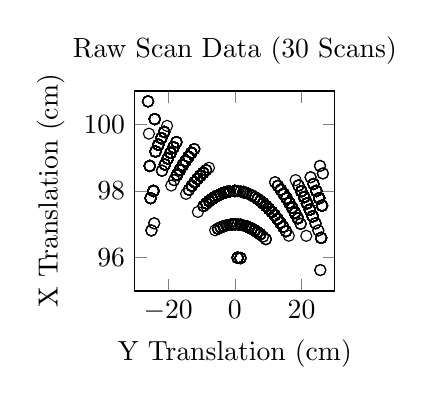
\begin{tikzpicture}

\begin{axis}[%
width=1in,
height=1in,
scale only axis,
xmin=-30,
xmax=30,
xlabel={Y Translation (cm)},
ymin=95,
ymax=101,
ylabel={X Translation (cm)},
title={Raw Scan Data (30 Scans)}
]
\addplot [
color=black,
only marks,
mark=o,
mark options={solid},
forget plot
]
table[row sep=crcr]{
25.8819 96.59258\\
26.14072 97.55851\\
26.14072 97.55851\\
25.8819 96.59258\\
25.8819 96.59258\\
26.14072 97.55851\\
26.14072 97.55851\\
25.8819 96.59258\\
25.8819 96.59258\\
26.14072 97.55851\\
26.14072 97.55851\\
26.39954 98.52443\\
26.14072 97.55851\\
25.8819 96.59258\\
26.14072 97.55851\\
26.39954 98.52443\\
26.14072 97.55851\\
26.14072 97.55851\\
26.14072 97.55851\\
25.8819 96.59258\\
26.14072 97.55851\\
26.14072 97.55851\\
25.8819 96.59258\\
25.62309 95.62666\\
25.8819 96.59258\\
25.8819 96.59258\\
25.62309 95.62666\\
26.14072 97.55851\\
26.14072 97.55851\\
26.14072 97.55851\\
};
\addplot [
color=black,
only marks,
mark=o,
mark options={solid},
forget plot
]
table[row sep=crcr]{
25.28838 97.78291\\
25.28838 97.78291\\
25.28838 97.78291\\
25.28838 97.78291\\
25.038 96.81476\\
25.28838 97.78291\\
25.53876 98.75106\\
25.28838 97.78291\\
25.28838 97.78291\\
25.28838 97.78291\\
25.038 96.81476\\
25.28838 97.78291\\
25.28838 97.78291\\
25.28838 97.78291\\
25.53876 98.75106\\
25.28838 97.78291\\
25.28838 97.78291\\
25.28838 97.78291\\
25.28838 97.78291\\
25.28838 97.78291\\
25.28838 97.78291\\
25.28838 97.78291\\
25.28838 97.78291\\
25.28838 97.78291\\
25.28838 97.78291\\
25.28838 97.78291\\
25.28838 97.78291\\
25.28838 97.78291\\
25.28838 97.78291\\
25.28838 97.78291\\
};
\addplot [
color=black,
only marks,
mark=o,
mark options={solid},
forget plot
]
table[row sep=crcr]{
24.43411 97.99987\\
24.19219 97.02957\\
24.43411 97.99987\\
24.43411 97.99987\\
24.43411 97.99987\\
24.43411 97.99987\\
24.43411 97.99987\\
24.43411 97.99987\\
24.19219 97.02957\\
24.43411 97.99987\\
24.43411 97.99987\\
24.43411 97.99987\\
24.43411 97.99987\\
24.43411 97.99987\\
24.43411 97.99987\\
24.19219 97.02957\\
24.43411 97.99987\\
24.43411 97.99987\\
24.43411 97.99987\\
24.43411 97.99987\\
24.19219 97.02957\\
24.43411 97.99987\\
24.43411 97.99987\\
24.43411 97.99987\\
24.43411 97.99987\\
24.43411 97.99987\\
24.43411 97.99987\\
24.43411 97.99987\\
24.43411 97.99987\\
24.43411 97.99987\\
};
\addplot [
color=black,
only marks,
mark=o,
mark options={solid},
forget plot
]
table[row sep=crcr]{
23.34454 97.23699\\
23.57798 98.20936\\
23.34454 97.23699\\
23.57798 98.20936\\
23.34454 97.23699\\
23.34454 97.23699\\
23.57798 98.20936\\
23.34454 97.23699\\
23.34454 97.23699\\
23.34454 97.23699\\
23.34454 97.23699\\
23.34454 97.23699\\
23.57798 98.20936\\
23.34454 97.23699\\
23.34454 97.23699\\
23.34454 97.23699\\
23.34454 97.23699\\
23.34454 97.23699\\
23.34454 97.23699\\
23.34454 97.23699\\
23.57798 98.20936\\
23.34454 97.23699\\
23.34454 97.23699\\
23.57798 98.20936\\
23.34454 97.23699\\
23.34454 97.23699\\
23.34454 97.23699\\
23.57798 98.20936\\
23.34454 97.23699\\
23.34454 97.23699\\
};
\addplot [
color=black,
only marks,
mark=o,
mark options={solid},
forget plot
]
table[row sep=crcr]{
22.49511 97.43701\\
22.49511 97.43701\\
22.49511 97.43701\\
22.49511 97.43701\\
22.49511 97.43701\\
22.49511 97.43701\\
22.49511 97.43701\\
22.72006 98.41138\\
22.49511 97.43701\\
22.49511 97.43701\\
22.49511 97.43701\\
22.49511 97.43701\\
22.49511 97.43701\\
22.49511 97.43701\\
22.49511 97.43701\\
22.49511 97.43701\\
22.49511 97.43701\\
22.49511 97.43701\\
22.49511 97.43701\\
22.72006 98.41138\\
22.49511 97.43701\\
22.49511 97.43701\\
22.49511 97.43701\\
22.49511 97.43701\\
22.49511 97.43701\\
22.49511 97.43701\\
22.49511 97.43701\\
22.49511 97.43701\\
22.49511 97.43701\\
22.49511 97.43701\\
};
\addplot [
color=black,
only marks,
mark=o,
mark options={solid},
forget plot
]
table[row sep=crcr]{
21.64396 97.6296\\
21.64396 97.6296\\
21.64396 97.6296\\
21.64396 97.6296\\
21.64396 97.6296\\
21.64396 97.6296\\
21.64396 97.6296\\
21.64396 97.6296\\
21.64396 97.6296\\
21.42752 96.6533\\
21.64396 97.6296\\
21.64396 97.6296\\
21.64396 97.6296\\
21.64396 97.6296\\
21.64396 97.6296\\
21.64396 97.6296\\
21.64396 97.6296\\
21.64396 97.6296\\
21.64396 97.6296\\
21.64396 97.6296\\
21.64396 97.6296\\
21.64396 97.6296\\
21.64396 97.6296\\
21.64396 97.6296\\
21.64396 97.6296\\
21.64396 97.6296\\
21.64396 97.6296\\
21.64396 97.6296\\
21.64396 97.6296\\
21.64396 97.6296\\
};
\addplot [
color=black,
only marks,
mark=o,
mark options={solid},
forget plot
]
table[row sep=crcr]{
20.79117 97.81476\\
20.79117 97.81476\\
20.79117 97.81476\\
20.79117 97.81476\\
20.79117 97.81476\\
20.79117 97.81476\\
20.79117 97.81476\\
20.79117 97.81476\\
20.79117 97.81476\\
20.79117 97.81476\\
20.79117 97.81476\\
20.79117 97.81476\\
20.79117 97.81476\\
20.79117 97.81476\\
20.79117 97.81476\\
20.79117 97.81476\\
20.79117 97.81476\\
20.79117 97.81476\\
20.79117 97.81476\\
20.79117 97.81476\\
20.79117 97.81476\\
20.79117 97.81476\\
20.79117 97.81476\\
20.79117 97.81476\\
20.79117 97.81476\\
20.79117 97.81476\\
20.79117 97.81476\\
20.79117 97.81476\\
20.79117 97.81476\\
20.79117 97.81476\\
};
\addplot [
color=black,
only marks,
mark=o,
mark options={solid},
forget plot
]
table[row sep=crcr]{
19.93679 97.99247\\
19.93679 97.99247\\
19.93679 97.99247\\
19.73743 97.01255\\
19.93679 97.99247\\
19.93679 97.99247\\
19.93679 97.99247\\
19.93679 97.99247\\
19.73743 97.01255\\
19.93679 97.99247\\
19.93679 97.99247\\
19.93679 97.99247\\
19.93679 97.99247\\
19.93679 97.99247\\
19.93679 97.99247\\
19.73743 97.01255\\
19.93679 97.99247\\
19.93679 97.99247\\
19.93679 97.99247\\
19.93679 97.99247\\
19.93679 97.99247\\
19.93679 97.99247\\
19.93679 97.99247\\
19.93679 97.99247\\
19.93679 97.99247\\
19.93679 97.99247\\
19.93679 97.99247\\
19.93679 97.99247\\
19.93679 97.99247\\
19.93679 97.99247\\
};
\addplot [
color=black,
only marks,
mark=o,
mark options={solid},
forget plot
]
table[row sep=crcr]{
18.89009 97.18109\\
18.89009 97.18109\\
19.0809 98.16272\\
18.89009 97.18109\\
18.89009 97.18109\\
19.0809 98.16272\\
18.89009 97.18109\\
18.89009 97.18109\\
18.89009 97.18109\\
18.89009 97.18109\\
18.89009 97.18109\\
18.89009 97.18109\\
18.89009 97.18109\\
19.0809 98.16272\\
18.89009 97.18109\\
18.89009 97.18109\\
18.89009 97.18109\\
19.0809 98.16272\\
18.89009 97.18109\\
18.89009 97.18109\\
18.89009 97.18109\\
18.89009 97.18109\\
19.0809 98.16272\\
19.0809 98.16272\\
18.89009 97.18109\\
18.89009 97.18109\\
18.89009 97.18109\\
18.89009 97.18109\\
18.89009 97.18109\\
18.89009 97.18109\\
};
\addplot [
color=black,
only marks,
mark=o,
mark options={solid},
forget plot
]
table[row sep=crcr]{
18.04132 97.34224\\
18.04132 97.34224\\
18.04132 97.34224\\
18.04132 97.34224\\
18.04132 97.34224\\
18.04132 97.34224\\
18.04132 97.34224\\
18.04132 97.34224\\
18.04132 97.34224\\
18.04132 97.34224\\
18.04132 97.34224\\
18.04132 97.34224\\
18.04132 97.34224\\
18.04132 97.34224\\
18.04132 97.34224\\
18.04132 97.34224\\
18.04132 97.34224\\
18.04132 97.34224\\
18.04132 97.34224\\
18.04132 97.34224\\
18.04132 97.34224\\
18.04132 97.34224\\
18.22355 98.32549\\
18.04132 97.34224\\
18.04132 97.34224\\
18.04132 97.34224\\
18.04132 97.34224\\
18.04132 97.34224\\
18.04132 97.34224\\
18.04132 97.34224\\
};
\addplot [
color=black,
only marks,
mark=o,
mark options={solid},
forget plot
]
table[row sep=crcr]{
17.19117 97.49597\\
17.19117 97.49597\\
17.19117 97.49597\\
17.19117 97.49597\\
17.19117 97.49597\\
17.19117 97.49597\\
17.19117 97.49597\\
17.19117 97.49597\\
17.19117 97.49597\\
17.19117 97.49597\\
17.19117 97.49597\\
17.19117 97.49597\\
17.19117 97.49597\\
17.19117 97.49597\\
17.19117 97.49597\\
17.19117 97.49597\\
17.19117 97.49597\\
17.19117 97.49597\\
17.19117 97.49597\\
17.19117 97.49597\\
17.19117 97.49597\\
17.19117 97.49597\\
17.19117 97.49597\\
17.19117 97.49597\\
17.19117 97.49597\\
17.19117 97.49597\\
17.19117 97.49597\\
17.19117 97.49597\\
17.19117 97.49597\\
17.19117 97.49597\\
};
\addplot [
color=black,
only marks,
mark=o,
mark options={solid},
forget plot
]
table[row sep=crcr]{
16.33971 97.64227\\
16.33971 97.64227\\
16.33971 97.64227\\
16.33971 97.64227\\
16.33971 97.64227\\
16.33971 97.64227\\
16.33971 97.64227\\
16.33971 97.64227\\
16.33971 97.64227\\
16.33971 97.64227\\
16.33971 97.64227\\
16.33971 97.64227\\
16.33971 97.64227\\
16.33971 97.64227\\
16.33971 97.64227\\
16.17467 96.65599\\
16.33971 97.64227\\
16.33971 97.64227\\
16.33971 97.64227\\
16.33971 97.64227\\
16.33971 97.64227\\
16.33971 97.64227\\
16.33971 97.64227\\
16.33971 97.64227\\
16.33971 97.64227\\
16.33971 97.64227\\
16.33971 97.64227\\
16.33971 97.64227\\
16.33971 97.64227\\
16.33971 97.64227\\
};
\addplot [
color=black,
only marks,
mark=o,
mark options={solid},
forget plot
]
table[row sep=crcr]{
15.48701 97.78115\\
15.48701 97.78115\\
15.48701 97.78115\\
15.48701 97.78115\\
15.48701 97.78115\\
15.48701 97.78115\\
15.48701 97.78115\\
15.33058 96.79346\\
15.48701 97.78115\\
15.48701 97.78115\\
15.48701 97.78115\\
15.33058 96.79346\\
15.48701 97.78115\\
15.48701 97.78115\\
15.33058 96.79346\\
15.48701 97.78115\\
15.33058 96.79346\\
15.48701 97.78115\\
15.48701 97.78115\\
15.48701 97.78115\\
15.33058 96.79346\\
15.48701 97.78115\\
15.33058 96.79346\\
15.33058 96.79346\\
15.33058 96.79346\\
15.48701 97.78115\\
15.48701 97.78115\\
15.48701 97.78115\\
15.48701 97.78115\\
15.48701 97.78115\\
};
\addplot [
color=black,
only marks,
mark=o,
mark options={solid},
forget plot
]
table[row sep=crcr]{
14.63313 97.91257\\
14.63313 97.91257\\
14.63313 97.91257\\
14.63313 97.91257\\
14.63313 97.91257\\
14.48532 96.92355\\
14.48532 96.92355\\
14.63313 97.91257\\
14.63313 97.91257\\
14.63313 97.91257\\
14.63313 97.91257\\
14.48532 96.92355\\
14.48532 96.92355\\
14.63313 97.91257\\
14.63313 97.91257\\
14.63313 97.91257\\
14.63313 97.91257\\
14.63313 97.91257\\
14.48532 96.92355\\
14.63313 97.91257\\
14.63313 97.91257\\
14.48532 96.92355\\
14.63313 97.91257\\
14.63313 97.91257\\
14.48532 96.92355\\
14.63313 97.91257\\
14.48532 96.92355\\
14.63313 97.91257\\
14.63313 97.91257\\
14.63313 97.91257\\
};
\addplot [
color=black,
only marks,
mark=o,
mark options={solid},
forget plot
]
table[row sep=crcr]{
13.63896 97.04627\\
13.63896 97.04627\\
13.63896 97.04627\\
13.77814 98.03654\\
13.63896 97.04627\\
13.77814 98.03654\\
13.63896 97.04627\\
13.63896 97.04627\\
13.63896 97.04627\\
13.63896 97.04627\\
13.77814 98.03654\\
13.77814 98.03654\\
13.77814 98.03654\\
13.77814 98.03654\\
13.63896 97.04627\\
13.63896 97.04627\\
13.77814 98.03654\\
13.63896 97.04627\\
13.77814 98.03654\\
13.63896 97.04627\\
13.63896 97.04627\\
13.77814 98.03654\\
13.77814 98.03654\\
13.77814 98.03654\\
13.63896 97.04627\\
13.63896 97.04627\\
13.77814 98.03654\\
13.77814 98.03654\\
13.63896 97.04627\\
13.63896 97.04627\\
};
\addplot [
color=black,
only marks,
mark=o,
mark options={solid},
forget plot
]
table[row sep=crcr]{
12.79157 97.1616\\
12.79157 97.1616\\
12.79157 97.1616\\
12.92209 98.15304\\
12.79157 97.1616\\
12.79157 97.1616\\
12.79157 97.1616\\
12.79157 97.1616\\
12.92209 98.15304\\
12.79157 97.1616\\
12.79157 97.1616\\
12.79157 97.1616\\
12.79157 97.1616\\
12.92209 98.15304\\
12.79157 97.1616\\
12.92209 98.15304\\
12.79157 97.1616\\
12.79157 97.1616\\
12.79157 97.1616\\
12.79157 97.1616\\
12.92209 98.15304\\
12.79157 97.1616\\
12.92209 98.15304\\
12.79157 97.1616\\
12.79157 97.1616\\
12.79157 97.1616\\
12.79157 97.1616\\
12.79157 97.1616\\
12.79157 97.1616\\
12.79157 97.1616\\
};
\addplot [
color=black,
only marks,
mark=o,
mark options={solid},
forget plot
]
table[row sep=crcr]{
11.9432 97.26952\\
11.9432 97.26952\\
11.9432 97.26952\\
11.9432 97.26952\\
11.9432 97.26952\\
12.06506 98.26207\\
11.9432 97.26952\\
11.9432 97.26952\\
11.9432 97.26952\\
11.9432 97.26952\\
11.9432 97.26952\\
11.9432 97.26952\\
12.06506 98.26207\\
11.9432 97.26952\\
11.9432 97.26952\\
11.9432 97.26952\\
11.9432 97.26952\\
11.9432 97.26952\\
11.9432 97.26952\\
11.9432 97.26952\\
11.9432 97.26952\\
11.9432 97.26952\\
11.9432 97.26952\\
11.9432 97.26952\\
11.9432 97.26952\\
11.9432 97.26952\\
11.9432 97.26952\\
11.9432 97.26952\\
11.9432 97.26952\\
11.9432 97.26952\\
};
\addplot [
color=black,
only marks,
mark=o,
mark options={solid},
forget plot
]
table[row sep=crcr]{
11.09391 97.37004\\
11.09391 97.37004\\
11.09391 97.37004\\
11.09391 97.37004\\
11.09391 97.37004\\
11.09391 97.37004\\
11.09391 97.37004\\
11.09391 97.37004\\
11.09391 97.37004\\
11.09391 97.37004\\
11.09391 97.37004\\
11.09391 97.37004\\
11.09391 97.37004\\
11.09391 97.37004\\
11.09391 97.37004\\
11.09391 97.37004\\
11.09391 97.37004\\
11.09391 97.37004\\
11.09391 97.37004\\
11.09391 97.37004\\
11.09391 97.37004\\
11.09391 97.37004\\
11.09391 97.37004\\
11.09391 97.37004\\
11.09391 97.37004\\
11.09391 97.37004\\
11.09391 97.37004\\
11.09391 97.37004\\
11.09391 97.37004\\
11.09391 97.37004\\
};
\addplot [
color=black,
only marks,
mark=o,
mark options={solid},
forget plot
]
table[row sep=crcr]{
10.24379 97.46315\\
10.24379 97.46315\\
10.24379 97.46315\\
10.24379 97.46315\\
10.24379 97.46315\\
10.24379 97.46315\\
10.24379 97.46315\\
10.24379 97.46315\\
10.24379 97.46315\\
10.24379 97.46315\\
10.24379 97.46315\\
10.24379 97.46315\\
10.24379 97.46315\\
10.24379 97.46315\\
10.24379 97.46315\\
10.24379 97.46315\\
10.24379 97.46315\\
10.24379 97.46315\\
10.24379 97.46315\\
10.24379 97.46315\\
10.24379 97.46315\\
10.24379 97.46315\\
10.24379 97.46315\\
10.24379 97.46315\\
10.24379 97.46315\\
10.24379 97.46315\\
10.24379 97.46315\\
10.24379 97.46315\\
10.24379 97.46315\\
10.24379 97.46315\\
};
\addplot [
color=black,
only marks,
mark=o,
mark options={solid},
forget plot
]
table[row sep=crcr]{
9.392884 97.54883\\
9.392884 97.54883\\
9.392884 97.54883\\
9.392884 97.54883\\
9.392884 97.54883\\
9.392884 97.54883\\
9.392884 97.54883\\
9.392884 97.54883\\
9.297038 96.55343\\
9.297038 96.55343\\
9.392884 97.54883\\
9.392884 97.54883\\
9.392884 97.54883\\
9.392884 97.54883\\
9.392884 97.54883\\
9.392884 97.54883\\
9.392884 97.54883\\
9.297038 96.55343\\
9.392884 97.54883\\
9.392884 97.54883\\
9.392884 97.54883\\
9.392884 97.54883\\
9.392884 97.54883\\
9.392884 97.54883\\
9.392884 97.54883\\
9.392884 97.54883\\
9.392884 97.54883\\
9.392884 97.54883\\
9.392884 97.54883\\
9.392884 97.54883\\
};
\addplot [
color=black,
only marks,
mark=o,
mark options={solid},
forget plot
]
table[row sep=crcr]{
8.541263 97.62708\\
8.541263 97.62708\\
8.541263 97.62708\\
8.541263 97.62708\\
8.541263 97.62708\\
8.541263 97.62708\\
8.541263 97.62708\\
8.541263 97.62708\\
8.541263 97.62708\\
8.541263 97.62708\\
8.541263 97.62708\\
8.541263 97.62708\\
8.454107 96.63089\\
8.541263 97.62708\\
8.541263 97.62708\\
8.541263 97.62708\\
8.454107 96.63089\\
8.541263 97.62708\\
8.541263 97.62708\\
8.541263 97.62708\\
8.541263 97.62708\\
8.541263 97.62708\\
8.541263 97.62708\\
8.541263 97.62708\\
8.541263 97.62708\\
8.541263 97.62708\\
8.541263 97.62708\\
8.541263 97.62708\\
8.541263 97.62708\\
8.541263 97.62708\\
};
\addplot [
color=black,
only marks,
mark=o,
mark options={solid},
forget plot
]
table[row sep=crcr]{
7.610532 96.70098\\
7.688991 97.6979\\
7.688991 97.6979\\
7.688991 97.6979\\
7.688991 97.6979\\
7.610532 96.70098\\
7.610532 96.70098\\
7.688991 97.6979\\
7.610532 96.70098\\
7.610532 96.70098\\
7.610532 96.70098\\
7.688991 97.6979\\
7.610532 96.70098\\
7.610532 96.70098\\
7.610532 96.70098\\
7.688991 97.6979\\
7.610532 96.70098\\
7.688991 97.6979\\
7.610532 96.70098\\
7.688991 97.6979\\
7.610532 96.70098\\
7.688991 97.6979\\
7.610532 96.70098\\
7.610532 96.70098\\
7.688991 97.6979\\
7.688991 97.6979\\
7.688991 97.6979\\
7.688991 97.6979\\
7.688991 97.6979\\
7.688991 97.6979\\
};
\addplot [
color=black,
only marks,
mark=o,
mark options={solid},
forget plot
]
table[row sep=crcr]{
6.766378 96.76371\\
6.766378 96.76371\\
6.766378 96.76371\\
6.836134 97.76128\\
6.766378 96.76371\\
6.766378 96.76371\\
6.766378 96.76371\\
6.766378 96.76371\\
6.766378 96.76371\\
6.836134 97.76128\\
6.836134 97.76128\\
6.836134 97.76128\\
6.836134 97.76128\\
6.766378 96.76371\\
6.766378 96.76371\\
6.836134 97.76128\\
6.766378 96.76371\\
6.766378 96.76371\\
6.766378 96.76371\\
6.836134 97.76128\\
6.766378 96.76371\\
6.766378 96.76371\\
6.766378 96.76371\\
6.766378 96.76371\\
6.766378 96.76371\\
6.766378 96.76371\\
6.836134 97.76128\\
6.766378 96.76371\\
6.766378 96.76371\\
6.766378 96.76371\\
};
\addplot [
color=black,
only marks,
mark=o,
mark options={solid},
forget plot
]
table[row sep=crcr]{
5.921708 96.81908\\
5.921708 96.81908\\
5.921708 96.81908\\
5.921708 96.81908\\
5.921708 96.81908\\
5.921708 96.81908\\
5.921708 96.81908\\
5.921708 96.81908\\
5.921708 96.81908\\
5.982757 97.81721\\
5.921708 96.81908\\
5.982757 97.81721\\
5.921708 96.81908\\
5.921708 96.81908\\
5.921708 96.81908\\
5.921708 96.81908\\
5.921708 96.81908\\
5.921708 96.81908\\
5.921708 96.81908\\
5.982757 97.81721\\
5.921708 96.81908\\
5.921708 96.81908\\
5.921708 96.81908\\
5.921708 96.81908\\
5.921708 96.81908\\
5.982757 97.81721\\
5.921708 96.81908\\
5.921708 96.81908\\
5.921708 96.81908\\
5.921708 96.81908\\
};
\addplot [
color=black,
only marks,
mark=o,
mark options={solid},
forget plot
]
table[row sep=crcr]{
5.076588 96.86706\\
5.076588 96.86706\\
5.076588 96.86706\\
5.076588 96.86706\\
5.076588 96.86706\\
5.076588 96.86706\\
5.076588 96.86706\\
5.076588 96.86706\\
5.076588 96.86706\\
5.076588 96.86706\\
5.128924 97.86569\\
5.076588 96.86706\\
5.076588 96.86706\\
5.128924 97.86569\\
5.076588 96.86706\\
5.076588 96.86706\\
5.076588 96.86706\\
5.076588 96.86706\\
5.076588 96.86706\\
5.128924 97.86569\\
5.076588 96.86706\\
5.128924 97.86569\\
5.076588 96.86706\\
5.076588 96.86706\\
5.076588 96.86706\\
5.076588 96.86706\\
5.076588 96.86706\\
5.076588 96.86706\\
5.076588 96.86706\\
5.076588 96.86706\\
};
\addplot [
color=black,
only marks,
mark=o,
mark options={solid},
forget plot
]
table[row sep=crcr]{
4.231081 96.90768\\
4.231081 96.90768\\
4.231081 96.90768\\
4.231081 96.90768\\
4.231081 96.90768\\
4.231081 96.90768\\
4.231081 96.90768\\
4.231081 96.90768\\
4.231081 96.90768\\
4.231081 96.90768\\
4.231081 96.90768\\
4.2747 97.90673\\
4.231081 96.90768\\
4.231081 96.90768\\
4.231081 96.90768\\
4.231081 96.90768\\
4.231081 96.90768\\
4.231081 96.90768\\
4.231081 96.90768\\
4.231081 96.90768\\
4.231081 96.90768\\
4.231081 96.90768\\
4.231081 96.90768\\
4.231081 96.90768\\
4.231081 96.90768\\
4.231081 96.90768\\
4.231081 96.90768\\
4.231081 96.90768\\
4.231081 96.90768\\
4.231081 96.90768\\
};
\addplot [
color=black,
only marks,
mark=o,
mark options={solid},
forget plot
]
table[row sep=crcr]{
3.385251 96.94091\\
3.385251 96.94091\\
3.420151 97.9403\\
3.385251 96.94091\\
3.385251 96.94091\\
3.420151 97.9403\\
3.385251 96.94091\\
3.385251 96.94091\\
3.385251 96.94091\\
3.385251 96.94091\\
3.385251 96.94091\\
3.385251 96.94091\\
3.420151 97.9403\\
3.385251 96.94091\\
3.385251 96.94091\\
3.420151 97.9403\\
3.385251 96.94091\\
3.385251 96.94091\\
3.385251 96.94091\\
3.385251 96.94091\\
3.385251 96.94091\\
3.385251 96.94091\\
3.385251 96.94091\\
3.420151 97.9403\\
3.420151 97.9403\\
3.385251 96.94091\\
3.420151 97.9403\\
3.420151 97.9403\\
3.385251 96.94091\\
3.385251 96.94091\\
};
\addplot [
color=black,
only marks,
mark=o,
mark options={solid},
forget plot
]
table[row sep=crcr]{
2.565341 97.96642\\
2.565341 97.96642\\
2.565341 97.96642\\
2.565341 97.96642\\
2.565341 97.96642\\
2.565341 97.96642\\
2.565341 97.96642\\
2.565341 97.96642\\
2.565341 97.96642\\
2.565341 97.96642\\
2.565341 97.96642\\
2.565341 97.96642\\
2.565341 97.96642\\
2.565341 97.96642\\
2.565341 97.96642\\
2.565341 97.96642\\
2.539164 96.96676\\
2.565341 97.96642\\
2.565341 97.96642\\
2.565341 97.96642\\
2.565341 97.96642\\
2.565341 97.96642\\
2.565341 97.96642\\
2.565341 97.96642\\
2.565341 97.96642\\
2.565341 97.96642\\
2.565341 97.96642\\
2.565341 97.96642\\
2.565341 97.96642\\
2.565341 97.96642\\
};
\addplot [
color=black,
only marks,
mark=o,
mark options={solid},
forget plot
]
table[row sep=crcr]{
1.692883 96.98523\\
1.692883 96.98523\\
1.675431 95.98538\\
1.692883 96.98523\\
1.675431 95.98538\\
1.692883 96.98523\\
1.710336 97.98507\\
1.692883 96.98523\\
1.692883 96.98523\\
1.692883 96.98523\\
1.692883 96.98523\\
1.692883 96.98523\\
1.675431 95.98538\\
1.692883 96.98523\\
1.692883 96.98523\\
1.675431 95.98538\\
1.675431 95.98538\\
1.692883 96.98523\\
1.692883 96.98523\\
1.675431 95.98538\\
1.675431 95.98538\\
1.675431 95.98538\\
1.692883 96.98523\\
1.675431 95.98538\\
1.692883 96.98523\\
1.675431 95.98538\\
1.692883 96.98523\\
1.692883 96.98523\\
1.692883 96.98523\\
1.710336 97.98507\\
};
\addplot [
color=black,
only marks,
mark=o,
mark options={solid},
forget plot
]
table[row sep=crcr]{
0.8377474 95.99634\\
0.8464739 96.99631\\
0.8377474 95.99634\\
0.8552005 97.99627\\
0.8377474 95.99634\\
0.8377474 95.99634\\
0.8377474 95.99634\\
0.8377474 95.99634\\
0.8377474 95.99634\\
0.8377474 95.99634\\
0.8377474 95.99634\\
0.8377474 95.99634\\
0.8377474 95.99634\\
0.8377474 95.99634\\
0.8377474 95.99634\\
0.8377474 95.99634\\
0.8377474 95.99634\\
0.8377474 95.99634\\
0.8377474 95.99634\\
0.8377474 95.99634\\
0.8377474 95.99634\\
0.8377474 95.99634\\
0.8552005 97.99627\\
0.8464739 96.99631\\
0.8377474 95.99634\\
0.8464739 96.99631\\
0.8464739 96.99631\\
0.8377474 95.99634\\
0.8377474 95.99634\\
0.8377474 95.99634\\
};
\addplot [
color=black,
only marks,
mark=o,
mark options={solid},
forget plot
]
table[row sep=crcr]{
0 97\\
0 98\\
0 97\\
0 97\\
0 98\\
0 98\\
0 98\\
0 98\\
0 98\\
0 97\\
0 98\\
0 98\\
0 98\\
0 97\\
0 98\\
0 98\\
0 97\\
0 98\\
0 98\\
0 98\\
0 98\\
0 98\\
0 98\\
0 98\\
0 97\\
0 98\\
0 98\\
0 98\\
0 98\\
0 98\\
};
\addplot [
color=black,
only marks,
mark=o,
mark options={solid},
forget plot
]
table[row sep=crcr]{
-0.8464739 96.99631\\
-0.8464739 96.99631\\
-0.8464739 96.99631\\
-0.8464739 96.99631\\
-0.8464739 96.99631\\
-0.8464739 96.99631\\
-0.8464739 96.99631\\
-0.8464739 96.99631\\
-0.8464739 96.99631\\
-0.8464739 96.99631\\
-0.8464739 96.99631\\
-0.8464739 96.99631\\
-0.8464739 96.99631\\
-0.8464739 96.99631\\
-0.8464739 96.99631\\
-0.8464739 96.99631\\
-0.8464739 96.99631\\
-0.8464739 96.99631\\
-0.8464739 96.99631\\
-0.8464739 96.99631\\
-0.8464739 96.99631\\
-0.8464739 96.99631\\
-0.8464739 96.99631\\
-0.8464739 96.99631\\
-0.8464739 96.99631\\
-0.8464739 96.99631\\
-0.8464739 96.99631\\
-0.8464739 96.99631\\
-0.8464739 96.99631\\
-0.8464739 96.99631\\
};
\addplot [
color=black,
only marks,
mark=o,
mark options={solid},
forget plot
]
table[row sep=crcr]{
-1.710336 97.98507\\
-1.710336 97.98507\\
-1.710336 97.98507\\
-1.710336 97.98507\\
-1.710336 97.98507\\
-1.710336 97.98507\\
-1.710336 97.98507\\
-1.710336 97.98507\\
-1.710336 97.98507\\
-1.710336 97.98507\\
-1.692883 96.98523\\
-1.710336 97.98507\\
-1.710336 97.98507\\
-1.710336 97.98507\\
-1.710336 97.98507\\
-1.710336 97.98507\\
-1.710336 97.98507\\
-1.710336 97.98507\\
-1.710336 97.98507\\
-1.710336 97.98507\\
-1.710336 97.98507\\
-1.710336 97.98507\\
-1.710336 97.98507\\
-1.710336 97.98507\\
-1.710336 97.98507\\
-1.710336 97.98507\\
-1.710336 97.98507\\
-1.710336 97.98507\\
-1.710336 97.98507\\
-1.710336 97.98507\\
};
\addplot [
color=black,
only marks,
mark=o,
mark options={solid},
forget plot
]
table[row sep=crcr]{
-2.565341 97.96642\\
-2.565341 97.96642\\
-2.565341 97.96642\\
-2.565341 97.96642\\
-2.565341 97.96642\\
-2.565341 97.96642\\
-2.565341 97.96642\\
-2.565341 97.96642\\
-2.565341 97.96642\\
-2.565341 97.96642\\
-2.565341 97.96642\\
-2.565341 97.96642\\
-2.565341 97.96642\\
-2.565341 97.96642\\
-2.565341 97.96642\\
-2.565341 97.96642\\
-2.539164 96.96676\\
-2.539164 96.96676\\
-2.565341 97.96642\\
-2.539164 96.96676\\
-2.565341 97.96642\\
-2.565341 97.96642\\
-2.565341 97.96642\\
-2.565341 97.96642\\
-2.565341 97.96642\\
-2.565341 97.96642\\
-2.565341 97.96642\\
-2.565341 97.96642\\
-2.565341 97.96642\\
-2.565341 97.96642\\
};
\addplot [
color=black,
only marks,
mark=o,
mark options={solid},
forget plot
]
table[row sep=crcr]{
-3.420151 97.9403\\
-3.385251 96.94091\\
-3.420151 97.9403\\
-3.420151 97.9403\\
-3.420151 97.9403\\
-3.385251 96.94091\\
-3.385251 96.94091\\
-3.420151 97.9403\\
-3.385251 96.94091\\
-3.420151 97.9403\\
-3.420151 97.9403\\
-3.420151 97.9403\\
-3.420151 97.9403\\
-3.420151 97.9403\\
-3.420151 97.9403\\
-3.385251 96.94091\\
-3.420151 97.9403\\
-3.420151 97.9403\\
-3.420151 97.9403\\
-3.420151 97.9403\\
-3.420151 97.9403\\
-3.385251 96.94091\\
-3.385251 96.94091\\
-3.385251 96.94091\\
-3.385251 96.94091\\
-3.385251 96.94091\\
-3.420151 97.9403\\
-3.420151 97.9403\\
-3.420151 97.9403\\
-3.420151 97.9403\\
};
\addplot [
color=black,
only marks,
mark=o,
mark options={solid},
forget plot
]
table[row sep=crcr]{
-4.2747 97.90673\\
-4.2747 97.90673\\
-4.231081 96.90768\\
-4.2747 97.90673\\
-4.2747 97.90673\\
-4.2747 97.90673\\
-4.231081 96.90768\\
-4.2747 97.90673\\
-4.231081 96.90768\\
-4.2747 97.90673\\
-4.2747 97.90673\\
-4.2747 97.90673\\
-4.2747 97.90673\\
-4.231081 96.90768\\
-4.2747 97.90673\\
-4.2747 97.90673\\
-4.2747 97.90673\\
-4.2747 97.90673\\
-4.2747 97.90673\\
-4.231081 96.90768\\
-4.231081 96.90768\\
-4.231081 96.90768\\
-4.2747 97.90673\\
-4.2747 97.90673\\
-4.231081 96.90768\\
-4.2747 97.90673\\
-4.2747 97.90673\\
-4.2747 97.90673\\
-4.2747 97.90673\\
-4.231081 96.90768\\
};
\addplot [
color=black,
only marks,
mark=o,
mark options={solid},
forget plot
]
table[row sep=crcr]{
-5.128924 97.86569\\
-5.128924 97.86569\\
-5.128924 97.86569\\
-5.128924 97.86569\\
-5.128924 97.86569\\
-5.128924 97.86569\\
-5.128924 97.86569\\
-5.128924 97.86569\\
-5.128924 97.86569\\
-5.076588 96.86706\\
-5.128924 97.86569\\
-5.128924 97.86569\\
-5.128924 97.86569\\
-5.076588 96.86706\\
-5.076588 96.86706\\
-5.128924 97.86569\\
-5.128924 97.86569\\
-5.076588 96.86706\\
-5.128924 97.86569\\
-5.128924 97.86569\\
-5.076588 96.86706\\
-5.128924 97.86569\\
-5.128924 97.86569\\
-5.128924 97.86569\\
-5.128924 97.86569\\
-5.128924 97.86569\\
-5.128924 97.86569\\
-5.128924 97.86569\\
-5.128924 97.86569\\
-5.128924 97.86569\\
};
\addplot [
color=black,
only marks,
mark=o,
mark options={solid},
forget plot
]
table[row sep=crcr]{
-5.982757 97.81721\\
-5.982757 97.81721\\
-5.982757 97.81721\\
-5.982757 97.81721\\
-5.982757 97.81721\\
-5.982757 97.81721\\
-5.982757 97.81721\\
-5.982757 97.81721\\
-5.982757 97.81721\\
-5.982757 97.81721\\
-5.982757 97.81721\\
-5.982757 97.81721\\
-5.982757 97.81721\\
-5.982757 97.81721\\
-5.982757 97.81721\\
-5.982757 97.81721\\
-5.982757 97.81721\\
-5.982757 97.81721\\
-5.982757 97.81721\\
-5.982757 97.81721\\
-5.982757 97.81721\\
-5.982757 97.81721\\
-5.982757 97.81721\\
-5.982757 97.81721\\
-5.921708 96.81908\\
-5.982757 97.81721\\
-5.982757 97.81721\\
-5.982757 97.81721\\
-5.982757 97.81721\\
-5.982757 97.81721\\
};
\addplot [
color=black,
only marks,
mark=o,
mark options={solid},
forget plot
]
table[row sep=crcr]{
-6.836134 97.76128\\
-6.836134 97.76128\\
-6.836134 97.76128\\
-6.836134 97.76128\\
-6.836134 97.76128\\
-6.836134 97.76128\\
-6.836134 97.76128\\
-6.836134 97.76128\\
-6.836134 97.76128\\
-6.836134 97.76128\\
-6.836134 97.76128\\
-6.836134 97.76128\\
-6.836134 97.76128\\
-6.836134 97.76128\\
-6.836134 97.76128\\
-6.836134 97.76128\\
-6.836134 97.76128\\
-6.836134 97.76128\\
-6.836134 97.76128\\
-6.836134 97.76128\\
-6.836134 97.76128\\
-6.836134 97.76128\\
-6.836134 97.76128\\
-6.836134 97.76128\\
-6.836134 97.76128\\
-6.836134 97.76128\\
-6.836134 97.76128\\
-6.836134 97.76128\\
-6.836134 97.76128\\
-6.836134 97.76128\\
};
\addplot [
color=black,
only marks,
mark=o,
mark options={solid},
forget plot
]
table[row sep=crcr]{
-7.688991 97.6979\\
-7.688991 97.6979\\
-7.688991 97.6979\\
-7.688991 97.6979\\
-7.688991 97.6979\\
-7.688991 97.6979\\
-7.688991 97.6979\\
-7.688991 97.6979\\
-7.688991 97.6979\\
-7.688991 97.6979\\
-7.688991 97.6979\\
-7.688991 97.6979\\
-7.688991 97.6979\\
-7.688991 97.6979\\
-7.76745 98.69482\\
-7.688991 97.6979\\
-7.688991 97.6979\\
-7.688991 97.6979\\
-7.688991 97.6979\\
-7.688991 97.6979\\
-7.688991 97.6979\\
-7.688991 97.6979\\
-7.688991 97.6979\\
-7.688991 97.6979\\
-7.688991 97.6979\\
-7.688991 97.6979\\
-7.688991 97.6979\\
-7.688991 97.6979\\
-7.688991 97.6979\\
-7.688991 97.6979\\
};
\addplot [
color=black,
only marks,
mark=o,
mark options={solid},
forget plot
]
table[row sep=crcr]{
-8.541263 97.62708\\
-8.541263 97.62708\\
-8.541263 97.62708\\
-8.541263 97.62708\\
-8.541263 97.62708\\
-8.628419 98.62328\\
-8.541263 97.62708\\
-8.541263 97.62708\\
-8.541263 97.62708\\
-8.541263 97.62708\\
-8.541263 97.62708\\
-8.541263 97.62708\\
-8.541263 97.62708\\
-8.541263 97.62708\\
-8.541263 97.62708\\
-8.628419 98.62328\\
-8.541263 97.62708\\
-8.541263 97.62708\\
-8.541263 97.62708\\
-8.541263 97.62708\\
-8.541263 97.62708\\
-8.541263 97.62708\\
-8.541263 97.62708\\
-8.541263 97.62708\\
-8.541263 97.62708\\
-8.541263 97.62708\\
-8.541263 97.62708\\
-8.628419 98.62328\\
-8.628419 98.62328\\
-8.541263 97.62708\\
};
\addplot [
color=black,
only marks,
mark=o,
mark options={solid},
forget plot
]
table[row sep=crcr]{
-9.392884 97.54883\\
-9.488729 98.54422\\
-9.392884 97.54883\\
-9.488729 98.54422\\
-9.488729 98.54422\\
-9.392884 97.54883\\
-9.392884 97.54883\\
-9.488729 98.54422\\
-9.488729 98.54422\\
-9.488729 98.54422\\
-9.392884 97.54883\\
-9.488729 98.54422\\
-9.488729 98.54422\\
-9.488729 98.54422\\
-9.488729 98.54422\\
-9.488729 98.54422\\
-9.488729 98.54422\\
-9.488729 98.54422\\
-9.488729 98.54422\\
-9.488729 98.54422\\
-9.392884 97.54883\\
-9.488729 98.54422\\
-9.488729 98.54422\\
-9.488729 98.54422\\
-9.488729 98.54422\\
-9.488729 98.54422\\
-9.488729 98.54422\\
-9.488729 98.54422\\
-9.488729 98.54422\\
-9.488729 98.54422\\
};
\addplot [
color=black,
only marks,
mark=o,
mark options={solid},
forget plot
]
table[row sep=crcr]{
-10.34832 98.45767\\
-10.34832 98.45767\\
-10.34832 98.45767\\
-10.34832 98.45767\\
-10.34832 98.45767\\
-10.34832 98.45767\\
-10.34832 98.45767\\
-10.34832 98.45767\\
-10.34832 98.45767\\
-10.34832 98.45767\\
-10.34832 98.45767\\
-10.34832 98.45767\\
-10.34832 98.45767\\
-10.34832 98.45767\\
-10.34832 98.45767\\
-10.34832 98.45767\\
-10.34832 98.45767\\
-10.34832 98.45767\\
-10.34832 98.45767\\
-10.34832 98.45767\\
-10.34832 98.45767\\
-10.34832 98.45767\\
-10.34832 98.45767\\
-10.34832 98.45767\\
-10.34832 98.45767\\
-10.34832 98.45767\\
-10.34832 98.45767\\
-10.34832 98.45767\\
-10.34832 98.45767\\
-10.34832 98.45767\\
};
\addplot [
color=black,
only marks,
mark=o,
mark options={solid},
forget plot
]
table[row sep=crcr]{
-11.20712 98.36361\\
-11.20712 98.36361\\
-11.20712 98.36361\\
-11.20712 98.36361\\
-11.20712 98.36361\\
-11.20712 98.36361\\
-11.20712 98.36361\\
-11.20712 98.36361\\
-11.09391 97.37004\\
-11.20712 98.36361\\
-11.20712 98.36361\\
-11.20712 98.36361\\
-11.20712 98.36361\\
-11.20712 98.36361\\
-11.20712 98.36361\\
-11.20712 98.36361\\
-11.20712 98.36361\\
-11.20712 98.36361\\
-11.20712 98.36361\\
-11.20712 98.36361\\
-11.20712 98.36361\\
-11.20712 98.36361\\
-11.20712 98.36361\\
-11.20712 98.36361\\
-11.20712 98.36361\\
-11.20712 98.36361\\
-11.20712 98.36361\\
-11.20712 98.36361\\
-11.20712 98.36361\\
-11.20712 98.36361\\
};
\addplot [
color=black,
only marks,
mark=o,
mark options={solid},
forget plot
]
table[row sep=crcr]{
-12.18693 99.25462\\
-12.06506 98.26207\\
-12.06506 98.26207\\
-12.18693 99.25462\\
-12.06506 98.26207\\
-12.06506 98.26207\\
-12.06506 98.26207\\
-12.06506 98.26207\\
-12.06506 98.26207\\
-12.06506 98.26207\\
-12.06506 98.26207\\
-12.06506 98.26207\\
-12.06506 98.26207\\
-12.06506 98.26207\\
-12.18693 99.25462\\
-12.06506 98.26207\\
-12.18693 99.25462\\
-12.06506 98.26207\\
-12.06506 98.26207\\
-12.06506 98.26207\\
-12.06506 98.26207\\
-12.06506 98.26207\\
-12.06506 98.26207\\
-12.06506 98.26207\\
-12.06506 98.26207\\
-12.06506 98.26207\\
-12.06506 98.26207\\
-12.06506 98.26207\\
-12.06506 98.26207\\
-12.06506 98.26207\\
};
\addplot [
color=black,
only marks,
mark=o,
mark options={solid},
forget plot
]
table[row sep=crcr]{
-13.05262 99.14449\\
-13.05262 99.14449\\
-12.92209 98.15304\\
-13.05262 99.14449\\
-12.92209 98.15304\\
-13.05262 99.14449\\
-12.92209 98.15304\\
-12.92209 98.15304\\
-13.05262 99.14449\\
-13.05262 99.14449\\
-12.92209 98.15304\\
-13.05262 99.14449\\
-12.92209 98.15304\\
-12.92209 98.15304\\
-12.92209 98.15304\\
-13.05262 99.14449\\
-12.92209 98.15304\\
-12.92209 98.15304\\
-13.05262 99.14449\\
-12.92209 98.15304\\
-12.92209 98.15304\\
-13.05262 99.14449\\
-13.05262 99.14449\\
-13.05262 99.14449\\
-13.05262 99.14449\\
-13.05262 99.14449\\
-13.05262 99.14449\\
-13.05262 99.14449\\
-13.05262 99.14449\\
-12.92209 98.15304\\
};
\addplot [
color=black,
only marks,
mark=o,
mark options={solid},
forget plot
]
table[row sep=crcr]{
-13.91731 99.02681\\
-13.91731 99.02681\\
-13.91731 99.02681\\
-13.91731 99.02681\\
-13.77814 98.03654\\
-13.77814 98.03654\\
-13.91731 99.02681\\
-13.91731 99.02681\\
-13.77814 98.03654\\
-13.91731 99.02681\\
-13.91731 99.02681\\
-13.91731 99.02681\\
-13.91731 99.02681\\
-13.91731 99.02681\\
-13.91731 99.02681\\
-13.91731 99.02681\\
-13.91731 99.02681\\
-13.91731 99.02681\\
-13.77814 98.03654\\
-13.91731 99.02681\\
-13.91731 99.02681\\
-13.91731 99.02681\\
-13.91731 99.02681\\
-13.91731 99.02681\\
-13.91731 99.02681\\
-13.91731 99.02681\\
-13.91731 99.02681\\
-13.91731 99.02681\\
-13.91731 99.02681\\
-13.91731 99.02681\\
};
\addplot [
color=black,
only marks,
mark=o,
mark options={solid},
forget plot
]
table[row sep=crcr]{
-14.78094 98.90159\\
-14.78094 98.90159\\
-14.78094 98.90159\\
-14.78094 98.90159\\
-14.78094 98.90159\\
-14.78094 98.90159\\
-14.78094 98.90159\\
-14.78094 98.90159\\
-14.78094 98.90159\\
-14.78094 98.90159\\
-14.78094 98.90159\\
-14.78094 98.90159\\
-14.78094 98.90159\\
-14.78094 98.90159\\
-14.78094 98.90159\\
-14.78094 98.90159\\
-14.78094 98.90159\\
-14.78094 98.90159\\
-14.78094 98.90159\\
-14.78094 98.90159\\
-14.78094 98.90159\\
-14.78094 98.90159\\
-14.78094 98.90159\\
-14.78094 98.90159\\
-14.78094 98.90159\\
-14.78094 98.90159\\
-14.78094 98.90159\\
-14.78094 98.90159\\
-14.78094 98.90159\\
-14.63313 97.91257\\
};
\addplot [
color=black,
only marks,
mark=o,
mark options={solid},
forget plot
]
table[row sep=crcr]{
-15.64345 98.76883\\
-15.64345 98.76883\\
-15.64345 98.76883\\
-15.64345 98.76883\\
-15.64345 98.76883\\
-15.64345 98.76883\\
-15.64345 98.76883\\
-15.64345 98.76883\\
-15.64345 98.76883\\
-15.64345 98.76883\\
-15.64345 98.76883\\
-15.64345 98.76883\\
-15.64345 98.76883\\
-15.64345 98.76883\\
-15.64345 98.76883\\
-15.64345 98.76883\\
-15.64345 98.76883\\
-15.64345 98.76883\\
-15.64345 98.76883\\
-15.64345 98.76883\\
-15.64345 98.76883\\
-15.64345 98.76883\\
-15.64345 98.76883\\
-15.64345 98.76883\\
-15.64345 98.76883\\
-15.64345 98.76883\\
-15.64345 98.76883\\
-15.64345 98.76883\\
-15.64345 98.76883\\
-15.64345 98.76883\\
};
\addplot [
color=black,
only marks,
mark=o,
mark options={solid},
forget plot
]
table[row sep=crcr]{
-16.50476 98.62856\\
-16.50476 98.62856\\
-16.50476 98.62856\\
-16.50476 98.62856\\
-16.50476 98.62856\\
-16.50476 98.62856\\
-16.50476 98.62856\\
-16.50476 98.62856\\
-16.50476 98.62856\\
-16.50476 98.62856\\
-16.50476 98.62856\\
-16.50476 98.62856\\
-16.50476 98.62856\\
-16.50476 98.62856\\
-16.50476 98.62856\\
-16.50476 98.62856\\
-16.50476 98.62856\\
-16.50476 98.62856\\
-16.50476 98.62856\\
-16.50476 98.62856\\
-16.50476 98.62856\\
-16.50476 98.62856\\
-16.50476 98.62856\\
-16.50476 98.62856\\
-16.50476 98.62856\\
-16.50476 98.62856\\
-16.50476 98.62856\\
-16.50476 98.62856\\
-16.50476 98.62856\\
-16.50476 98.62856\\
};
\addplot [
color=black,
only marks,
mark=o,
mark options={solid},
forget plot
]
table[row sep=crcr]{
-17.36482 98.48078\\
-17.36482 98.48078\\
-17.36482 98.48078\\
-17.53847 99.46558\\
-17.36482 98.48078\\
-17.36482 98.48078\\
-17.36482 98.48078\\
-17.36482 98.48078\\
-17.36482 98.48078\\
-17.53847 99.46558\\
-17.53847 99.46558\\
-17.36482 98.48078\\
-17.36482 98.48078\\
-17.53847 99.46558\\
-17.36482 98.48078\\
-17.36482 98.48078\\
-17.36482 98.48078\\
-17.36482 98.48078\\
-17.36482 98.48078\\
-17.53847 99.46558\\
-17.36482 98.48078\\
-17.53847 99.46558\\
-17.36482 98.48078\\
-17.36482 98.48078\\
-17.36482 98.48078\\
-17.36482 98.48078\\
-17.36482 98.48078\\
-17.36482 98.48078\\
-17.53847 99.46558\\
-17.36482 98.48078\\
};
\addplot [
color=black,
only marks,
mark=o,
mark options={solid},
forget plot
]
table[row sep=crcr]{
-18.40579 99.30875\\
-18.40579 99.30875\\
-18.40579 99.30875\\
-18.40579 99.30875\\
-18.40579 99.30875\\
-18.40579 99.30875\\
-18.40579 99.30875\\
-18.40579 99.30875\\
-18.40579 99.30875\\
-18.40579 99.30875\\
-18.40579 99.30875\\
-18.40579 99.30875\\
-18.40579 99.30875\\
-18.40579 99.30875\\
-18.40579 99.30875\\
-18.40579 99.30875\\
-18.40579 99.30875\\
-18.40579 99.30875\\
-18.40579 99.30875\\
-18.40579 99.30875\\
-18.40579 99.30875\\
-18.22355 98.32549\\
-18.22355 98.32549\\
-18.40579 99.30875\\
-18.40579 99.30875\\
-18.40579 99.30875\\
-18.40579 99.30875\\
-18.40579 99.30875\\
-18.40579 99.30875\\
-18.40579 99.30875\\
};
\addplot [
color=black,
only marks,
mark=o,
mark options={solid},
forget plot
]
table[row sep=crcr]{
-19.27171 99.14435\\
-19.27171 99.14435\\
-19.27171 99.14435\\
-19.27171 99.14435\\
-19.27171 99.14435\\
-19.27171 99.14435\\
-19.27171 99.14435\\
-19.0809 98.16272\\
-19.27171 99.14435\\
-19.27171 99.14435\\
-19.27171 99.14435\\
-19.27171 99.14435\\
-19.27171 99.14435\\
-19.27171 99.14435\\
-19.27171 99.14435\\
-19.27171 99.14435\\
-19.27171 99.14435\\
-19.27171 99.14435\\
-19.27171 99.14435\\
-19.27171 99.14435\\
-19.27171 99.14435\\
-19.27171 99.14435\\
-19.27171 99.14435\\
-19.27171 99.14435\\
-19.27171 99.14435\\
-19.27171 99.14435\\
-19.27171 99.14435\\
-19.27171 99.14435\\
-19.27171 99.14435\\
-19.27171 99.14435\\
};
\addplot [
color=black,
only marks,
mark=o,
mark options={solid},
forget plot
]
table[row sep=crcr]{
-20.13616 98.9724\\
-20.13616 98.9724\\
-20.13616 98.9724\\
-20.13616 98.9724\\
-20.13616 98.9724\\
-20.13616 98.9724\\
-20.13616 98.9724\\
-20.13616 98.9724\\
-20.13616 98.9724\\
-20.13616 98.9724\\
-20.13616 98.9724\\
-20.13616 98.9724\\
-20.13616 98.9724\\
-20.13616 98.9724\\
-20.13616 98.9724\\
-20.13616 98.9724\\
-20.33553 99.95232\\
-20.13616 98.9724\\
-20.13616 98.9724\\
-20.13616 98.9724\\
-20.13616 98.9724\\
-20.13616 98.9724\\
-20.13616 98.9724\\
-20.13616 98.9724\\
-20.13616 98.9724\\
-20.13616 98.9724\\
-20.13616 98.9724\\
-20.13616 98.9724\\
-20.13616 98.9724\\
-20.13616 98.9724\\
};
\addplot [
color=black,
only marks,
mark=o,
mark options={solid},
forget plot
]
table[row sep=crcr]{
-21.20699 99.77106\\
-20.99908 98.79291\\
-21.20699 99.77106\\
-20.99908 98.79291\\
-20.99908 98.79291\\
-21.20699 99.77106\\
-20.99908 98.79291\\
-20.99908 98.79291\\
-20.99908 98.79291\\
-20.99908 98.79291\\
-20.99908 98.79291\\
-21.20699 99.77106\\
-20.99908 98.79291\\
-20.99908 98.79291\\
-21.20699 99.77106\\
-21.20699 99.77106\\
-21.20699 99.77106\\
-21.20699 99.77106\\
-21.20699 99.77106\\
-21.20699 99.77106\\
-20.99908 98.79291\\
-20.99908 98.79291\\
-21.20699 99.77106\\
-21.20699 99.77106\\
-20.99908 98.79291\\
-21.20699 99.77106\\
-21.20699 99.77106\\
-21.20699 99.77106\\
-21.20699 99.77106\\
-21.20699 99.77106\\
};
\addplot [
color=black,
only marks,
mark=o,
mark options={solid},
forget plot
]
table[row sep=crcr]{
-22.07684 99.58219\\
-22.07684 99.58219\\
-22.07684 99.58219\\
-22.07684 99.58219\\
-22.07684 99.58219\\
-22.07684 99.58219\\
-22.07684 99.58219\\
-22.07684 99.58219\\
-22.07684 99.58219\\
-22.07684 99.58219\\
-22.07684 99.58219\\
-22.07684 99.58219\\
-22.07684 99.58219\\
-22.07684 99.58219\\
-22.07684 99.58219\\
-22.07684 99.58219\\
-21.8604 98.6059\\
-22.07684 99.58219\\
-22.07684 99.58219\\
-22.07684 99.58219\\
-22.07684 99.58219\\
-21.8604 98.6059\\
-22.07684 99.58219\\
-22.07684 99.58219\\
-22.07684 99.58219\\
-21.8604 98.6059\\
-22.07684 99.58219\\
-22.07684 99.58219\\
-22.07684 99.58219\\
-22.07684 99.58219\\
};
\addplot [
color=black,
only marks,
mark=o,
mark options={solid},
forget plot
]
table[row sep=crcr]{
-22.94501 99.38575\\
-22.94501 99.38575\\
-22.94501 99.38575\\
-22.94501 99.38575\\
-22.94501 99.38575\\
-22.94501 99.38575\\
-22.94501 99.38575\\
-22.94501 99.38575\\
-22.94501 99.38575\\
-22.94501 99.38575\\
-22.94501 99.38575\\
-22.94501 99.38575\\
-22.94501 99.38575\\
-22.94501 99.38575\\
-22.94501 99.38575\\
-22.94501 99.38575\\
-22.94501 99.38575\\
-22.94501 99.38575\\
-22.94501 99.38575\\
-22.94501 99.38575\\
-22.94501 99.38575\\
-22.94501 99.38575\\
-22.94501 99.38575\\
-22.94501 99.38575\\
-22.94501 99.38575\\
-22.94501 99.38575\\
-22.94501 99.38575\\
-22.94501 99.38575\\
-22.94501 99.38575\\
-22.94501 99.38575\\
};
\addplot [
color=black,
only marks,
mark=o,
mark options={solid},
forget plot
]
table[row sep=crcr]{
-23.81143 99.18173\\
-23.81143 99.18173\\
-23.81143 99.18173\\
-24.04487 100.1541\\
-23.81143 99.18173\\
-24.04487 100.1541\\
-23.81143 99.18173\\
-23.81143 99.18173\\
-24.04487 100.1541\\
-23.81143 99.18173\\
-24.04487 100.1541\\
-23.81143 99.18173\\
-24.04487 100.1541\\
-23.81143 99.18173\\
-23.81143 99.18173\\
-23.81143 99.18173\\
-23.81143 99.18173\\
-23.81143 99.18173\\
-23.81143 99.18173\\
-24.04487 100.1541\\
-23.81143 99.18173\\
-23.81143 99.18173\\
-24.04487 100.1541\\
-23.81143 99.18173\\
-23.81143 99.18173\\
-23.81143 99.18173\\
-24.04487 100.1541\\
-24.04487 100.1541\\
-24.04487 100.1541\\
-23.81143 99.18173\\
};
\addplot [
color=black,
only marks,
mark=o,
mark options={solid},
forget plot
]
table[row sep=crcr]{
-24.43411 97.99987\\
-24.43411 97.99987\\
-24.43411 97.99987\\
-24.43411 97.99987\\
-24.43411 97.99987\\
-24.43411 97.99987\\
-24.43411 97.99987\\
-24.43411 97.99987\\
-24.43411 97.99987\\
-24.43411 97.99987\\
-24.43411 97.99987\\
-24.43411 97.99987\\
-24.43411 97.99987\\
-24.19219 97.02957\\
-24.43411 97.99987\\
-24.43411 97.99987\\
-24.43411 97.99987\\
-24.43411 97.99987\\
-24.43411 97.99987\\
-24.43411 97.99987\\
-24.43411 97.99987\\
-24.43411 97.99987\\
-24.43411 97.99987\\
-24.19219 97.02957\\
-24.43411 97.99987\\
-24.43411 97.99987\\
-24.43411 97.99987\\
-24.43411 97.99987\\
-24.43411 97.99987\\
-24.43411 97.99987\\
};
\addplot [
color=black,
only marks,
mark=o,
mark options={solid},
forget plot
]
table[row sep=crcr]{
-25.53876 98.75106\\
-25.28838 97.78291\\
-25.28838 97.78291\\
-25.28838 97.78291\\
-25.28838 97.78291\\
-25.038 96.81476\\
-26.03952 100.6874\\
-25.53876 98.75106\\
-26.03952 100.6874\\
-26.03952 100.6874\\
-25.53876 98.75106\\
-25.53876 98.75106\\
-25.78914 99.71921\\
-25.53876 98.75106\\
-26.03952 100.6874\\
-25.53876 98.75106\\
-25.53876 98.75106\\
-25.53876 98.75106\\
-25.53876 98.75106\\
-25.28838 97.78291\\
-25.53876 98.75106\\
-25.28838 97.78291\\
-25.53876 98.75106\\
-25.28838 97.78291\\
-25.038 96.81476\\
-25.53876 98.75106\\
-25.53876 98.75106\\
-26.03952 100.6874\\
-25.28838 97.78291\\
-25.038 96.81476\\
};
\end{axis}
\end{tikzpicture}%
            \end{figure}
        \end{column}
    \end{columns} 
\end{frame}

% --------------------------------------------------- Future Work! --------------------------------------------------- %

\section{Future Directions}
\begin{frame}{Future Work}
    \begin{columns}[T]
        \begin{column}{.5\textwidth}
            \begin{itemize}
            \item{Construct a \alert{final target} from more rigid material}
            \item{Integrate a \alert{real-time heuristic} uncertainty propagation}
            \item{Verify method accuracy and precision with \alert{additional lidars}}
        \end{itemize}
        \end{column}
        \begin{column}{.5\textwidth}
            \begin{figure}
                \centering
                \includegraphics[width=\textwidth]{Images/pr2_map.jpg}
            \end{figure}
        \end{column}
    \end{columns} 
\end{frame}


\begin{frame}{Summary}
    \begin{enumerate}
        \item{Calibration is essential within the field of \alert{mobile robotics}}
        \item{We propose a \alert{closed-form} approach to calibration between two lidars using a newly designed target}
        \item{This approach reveals \alert{6DoF pose} using only 2D data}
    \end{enumerate}
    \begin{center}
        \fontsize{50pt}{10pt}\selectfont{ Questions?}
    \end{center}
\end{frame}

\end{document}